% This file was converted to LaTeX by Writer2LaTeX ver. 1.4
% see http://writer2latex.sourceforge.net for more info
\documentclass[a4paper]{article}
\usepackage[utf8]{inputenc}
\usepackage[T1]{fontenc}
\usepackage[ngerman]{babel}
\usepackage{amsmath}
\usepackage{amssymb,amsfonts,textcomp}
\usepackage{color}
\usepackage{array}
\usepackage{supertabular}
\usepackage{hhline}
\usepackage{hyperref}
% for environment subfigure
\usepackage{subcaption}
\usepackage{graphicx}
% Text styles
\newcommand\zitat[1]{\textit{#1}}

\newcommand{\img}[2][width=\linewidth]{%
  \noindent%
  \includegraphics[#1]{pictures/#2}%
}

\newcounter{Abb}
\renewcommand\theAbb{\arabic{Abb}}

\title{Josephs-Messe F-Dur op}
\begin{document}

{\centering\bfseries
Josef Friedrich
\par}

{\centering
\textbf{„Der Mozart von Ruhmannsfelden!“}
\par}

{\centering\bfseries
\textmd{Leben und Werk des Ruhmannsfeldener }
\par}

{\centering\bfseries
\textmd{Schulrektors, Heimatforschers und Komponisten }
\par}

{\centering\bfseries
\textmd{August Högn (1878 – 1961)}
\par}

{\centering
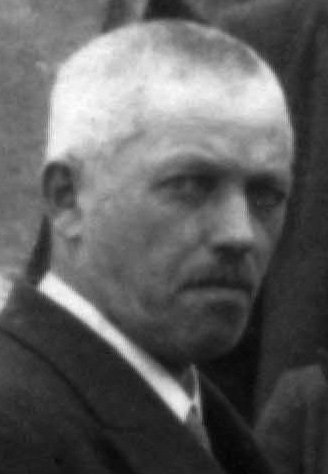
\includegraphics[width=3.836cm,height=5.556cm]{pictures/August-Hoegn_Nachruf.jpg}
 \par}
{\centering\bfseries
Band I: Hauptteil
\par}

{\centering
Zulassungsarbeit zur ersten Staatsprüfung für das Lehramt an Gymnasien,
\par}

{\centering
eingereicht bei Prof. Dr. Siegfried Mauser im Fach historische
Musikwissenschaft
\par}

{\centering
Ruhmannsfelden, München, April 2005
\par}

\clearpage{\bfseries
Inhaltsverzeichnis}

\subparagraph[Band I: Hauptteil]{Band I: Hauptteil}
\setcounter{tocdepth}{4}
\renewcommand\contentsname{}
\tableofcontents


\clearpage\setcounter{page}{1}\section{Vorwort}
\hypertarget{RefHeadingToc100333724}{}Als „Mozart von Ruhmannsfelden“
wurde August Högn in einer Ansprache an seinem 80. Geburtstag
bezeichnet. \footnote{Interview Nr. 24, Johann Glasschröder,
28.12.2004, Absatz 10} Der schmeichelnde Vergleich mit dem Salzburger
Komponisten war eine Verbeugung vor seinem jahrzehntelangen engagierten
Mitwirken am musikalischen Leben im kleinen Ort des Bayerischen Waldes
und besonders vor dem umfangreichen und in Ruhmannsfelden noch nie da
gewesenen kompositorischen Schaffen, auf das er zurückblicken konnte.
Auch ein beachtliches heimatkundliches Werk hatte er bis zu diesem
Zeitpunkt zusammengetragen und rechtfertige mehr als genug die weiteren
am letzten runden Geburtstag erteilten Ehren. Kaum größer könnte der
Unterschied zu Lebzeiten und heute sein, bezüglich der Würdigung seines
Schaffens und die Anerkennung seiner Dienste für die Allgemeinheit.
Fast 50 Jahre nach seinem Tod kennt kaum jemand der Ruhmannsfeldener
noch den Namen „August Högn“, geschweige denn sein musikalisches und
heimatkundliches Werk. Durch Zufall habe ich im Notenschrank der
Ruhmannsfeldener Pfarrkirche einige seiner Handschriften entdeckt, die
mein Interesse seinem Leben und Wirken erweckten und mich somit zu
Verfassen dieser Arbeit führten.

Ich möchte mit dieser Arbeit an das Leben und Werk des Rektors,
Heimatforschers und Komponisten August Högns erinnern, um somit seine
Person sowie Werk vor dem Vergessen zu bewahren. Da Högn sehr eng mit
meinem Heimatort Ruhmannsfelden verbunden war, wurde diese Arbeit fast
zwangsläufig zu einer „musikalischen Heimatkunde.“ Insofern kann man
die Arbeit auch als „Hommage an meine Heimat“ ansehen.

Bei der Erforschung von Högns Leben haben sich Berichte von Augenzeugen
als unverzichtbare Informationsquelle herausgestellt. Die Interviews
wurden mitgeschnitten (Daten-CD I) und transkribiert (Band II, Seite 7
- 56). Es war der letztmögliche Zeitpunkt durch Interviews mit
Zeitzeugen den hinter dem Werk stehenden Menschen aufzuzeigen. Der Tod
von zwei meiner meist hoch betagten Interviewpartner noch vor
Fertigstellung dieser Arbeit beweist eindringlich, wie schnell sich im
Laufe der Jahre die Spuren eines Menschen verwischen können, wenn sie
nicht rechtzeitig festgehalten werden.

Mehr als nur eine ergänzende Funktion zu den Interviews haben die in
eine Sammlung aufgenommen Dokumente. Ihnen ist es zu verdanken, dass
einige von Högns Lebensstationen, wie beispielsweise seine drei Phasen,
in denen er Chorregent war, zeitlich sehr genau bestimmt werden
konnten. Vor allem zum jungen Leben von Högn bildeten die Dokumente die
einzige Informationsquelle, da hier Augenzeugenberichte nicht mehr
möglich waren. Neben Dokumenten aus dem Gemeindearchiv waren besonders
die Archivalien, die das Pfarramt bereitstellen konnten, von
außerordentlichem Aufschlussreichtum in Bezug auf das Leben von August
Högn. Hier gab die „Chronik Ruhmannsfelden“ vom ehemaligen
Ruhmannsfeldener Pfarrer Franz Seraph Reicheneder nicht nur über Högns
Leben Auskunft, sondern auch über die Geschichte von Ruhmannsfelden.
Mancher Glücksfund erweitert zusätzlich das Spektrum an Schriftstücken,
zum Beispiel vier Briefe von Högn, die mir aus Australien übersandt
wurden. Sehr mühsam war die Entzifferung der in alter deutscher
Schreibschrift verfassten Dokumente. Einzige Möglichkeit, ihre Aussage
dauerhaft nachvollziehen zu können, blieb das Abschreiben. Da
handschriftliche Dokumente in der Sammlung überwiegen, habe ich mich
dazu entschlossen, alle Dokumente, auch die gut lesbaren, zu editieren.
So können alle Schriftstücke im Dokumentationsteil (Band II, Seite 57 -
90) wortwörtlich nachgelesen werden.

Der erste Teil dieser Arbeit handelt von Högns Leben. Eine Einbindung
und Bezugnahme von Högns musikalischem Werk in die Biographie war nicht
möglich, da man den Entstehungszeitpunkt der Kompositionen nur sehr
grob schätzen kann. Da sich sein Geschichtswerk hingegen sehr genau
zeitlich einordnen lässt und noch dazu viele Hintergrundinformationen
zur Entstehung bekannt sind, widmet sich ein Kapitel des ersten Teil
Högns heimatkundlichen Abhandlungen und ihrer Entstehung. Großer Wert
wurde auch auf die Abbildung der noch vorhandenen Fotos aus Högns
Privatleben gelegt, die große Aussagekraft leisten und den Text
auflockern.

Zum Erstellen des Werkverzeichnisses waren umfangreiche
Recherchearbeiten nötig. An mehreren unbekannten Plätzen lagerten Högns
Kompositionen, ehe sie ausfindig gemacht werden konnten. Die Anzahl der
Kompositionen steigerte sich im Laufe der Recherchearbeiten von den 12
Kompositionen aus dem Notenschrank in der Pfarrkirche Ruhmannsfelden,
dem ersten Fundort, auf fast 70 Werke. Um die tatsächliche Anzahl der
erhalten Werke festzustellen, musste der Kontakt zu Högns Nachfahren
hergestellt werden. Da alle Verbindungen zwischen der Ruhmannsfeldener
Bevölkerung sowie zwischen der Deggendorfer Verwandtschaft zu Högns
Enkelkindern abgerissen waren, gestaltete sich die Such nach den
Nachfahren entsprechend schwierig. Zwar besaßen die Nachfahren leider
auch keine Kompositionen mehr, doch konnte wenigstens die Suche als
beendet erklärt werden und das Werkverzeichnis bekam einen endgültigen
Charakter. Im Zuge der Durchsuchungsarbeiten nach Kompositionen am
Notenmaterial in der Pfarrkirche habe ich Listen aller Arrangements
(Seite \pageref{bkm:Ref100328080}) und aufgeführter Kompositionen (Band
II, Seite 99 - 101) von Högn angefertigt. Die Listen liefern eine
deutliche Abbildung von Högns musikalischem Umfeld und zeigen die
dadurch mögliche stilistische Beeinflussung auf Högns Werke auf. Einige
seiner Kompositionen wurden ediert (Band III) und lieferten den Anstoß
für etliche Wiederaufführungen (Band II, Seite 102 – 103, Daten-CD I).
Eine streng quellenbezogene Ausgabe der Werke mit kritischem Bericht
macht angesichts von Högns geringer Bedeutung in der Musikgeschichte
wenig Sinn. Stattdessen sollte das entstandene Notenmaterial mehr
aufführungspraktischen Überlegungen Rechnung tragen.

Der zweite Teil der Arbeit handelt vom musikalischen Werk Högns. Der
Beginn des Abschnitts „Werk“ ist vor allem um Rekonstruktion bemüht.
Fragen, die das Werkverzeichnis aufwirft, sollen hier beantwortet
werden. Abschließen wird auf einzelne Werke eingegangen. Da sich die
vorhergehenden Kapitel überwiegend mit der kirchenmusikalischen
Schaffen beschäftigt haben, wird dort auch auf seine weltliche
Kompositionen eingegangen. Neben seiner größten und wohl besten
geistlichen Komposition, der „Josephi“-Messe, erhalten auch die
weltlichen Kompositionen, nämlich der Marsch „In Treue fest!“ und der
Weihegesang Es-Dur ihren Platz. Högns einzig erhalte
nationalsozialistische Komposition soll bewusst nicht verschwiegen
werden. Ein Vergleich mit den geistlichen Grabliedern mag exemplarisch
darstellen, wie sich die damalige Propagandamusik Elemente aus anderen
Genres bediente.

Um Interessierten meine Forschungsergebnisse zugänglich zu mache, habe
ich eine Internetseite (www.august-hoegn.de) eingerichtet, die sich dem
Leben und Werk von August Högn widmet. Weitere noch zu verfolgende
Ziele wären eine Ausdehnung der regionalen Pflege seines musikalischen
Nachlasses von Ruhmannsfelden auf die Pfarreien das Dekanat Viechtach
und die Drucklegung einer heimatkundlichen Schrift über sein Leben und
Werk.

An dieser Stelle möchte ich mich bei den zahlreichen Personen bedanken,
die mir bei der Erforschung des Lebens und Werks von August Högn
behilflich waren. Ohne sie wäre diese Arbeit nicht möglich gewesen.
Eine Liste von über 40 am Projekt beteiligten Personen ist im Anhang
(Band II, Seite 104) zu finden.

München, April 2005\ \ \ \ \ \ \ \ Josef Friedrich

\section{Leben}

\subsection{Kindheit in
Deggendorf}


August Högn kam am 2. August 1878
in Deggendorf als Sohn von Andreas und Helene Högn, geborene Zöpfl, auf
die Welt. \footnote{Dokument Nr. 48, Zeitungsartikel aus Viechtacher
Bayerwald-Bote, 2.8.1958} August hatte zwei ältere Geschwister, Theres
(geboren 1869) und Ludwig (geboren 1871). Seine jüngeren Brüder, Joseph
und Otto, kamen 1879 und 1883 jeweils entsprechend auf die
Welt. \footnote{Grabinschrift der Familiengräber Andreas Högn und
Ludwig Högn am Deggendorfer Friedhof}

\begin{figure}
%
\begin{subfigure}[b]{0.5\linewidth}
\centering
\img[height=7cm]{Andreas-Hoegn}
\caption{Andreas Högn}
\end{subfigure}
%
\begin{subfigure}[b]{0.5\linewidth}
\centering
\img[height=7cm]{Helene-Hoegn}
\caption{Helene Högn}
\end{subfigure}
%
\caption{Die Eltern von August Högn}
\end{figure}

\begin{figure}
%
\begin{subfigure}[b]{0.5\linewidth}
\centering
\img[height=7cm]{Ludwig-Hoegn}
\caption{Ludwig Högn}
\end{subfigure}
%
\begin{subfigure}[b]{0.5\linewidth}
\centering
\img[height=7cm]{Joseph-Hoegn}
\caption{Joseph Högn}
\end{subfigure}
%
\caption{Zwei Brüder von August Högn}
\end{figure}

Augusts Vater war von Beruf Buchbinder und eröffnete zusammen mit seiner
Ehefrau 1867 eine Buchbinderei und Buchhandlung im so genannten
„Kerndel´schen-Haus“ am Luitpoldplatz in Deggendorf. Bereits nach 6
Jahren, also 1873, zog die Familie Högn in ein eigenes Haus in die
Pfleggasse 1, wo bis zum heutigen Tag die Buchhandlung Högn zu finden
ist (Abb. 5). Die äußerst günstige Lage der Buchhandlung im Zentrum
Deggendorfs war von bedeutendem wirtschaftlichen Vorteil. Besonders an
Markttagen, so zum Beispiel zum „Saumarkt“ in der Pfleggasse, strömten
viele Menschen aus der Umgebung nach Deggendorf, wovon auch die
Buchhandlung Högn profitierte. Das Sortiment wurde im Laufe der Zeit
erweitert und zusätzlich zu Büchern auch Schreib-, Schul-, Spiel- und
Lederwaren angeboten. Ab 1890 komplettierte ein eigener
Postkarten-Verlag das Angebot.\footnote{
http://www.hoegn.de/ueber/ueb\_gesch.php}

In dem Haus des späteren landgräflichen Magistratsrats, Landrats und
Landtagsabgeordneten \footnote{Grabinschrift des Familiengrabs Andreas
Högn am Deggendorfer Friedhof} Andreas Högn gehörte eine gründliche
Ausbildung und somit eine grundlegende musikalische Schulung der Kinder
allein schon zum guten Ton. Es ist daher kaum verwunderlich, dass alle
fünf Kinder das Klavierspielen erlernten, selbst der von Geburt an fast
taube Joseph Högn. \footnote{Interview Nr. 3, Ida Högn, 29.12.2002,
Absatz 40}

August Högn besuchte die Knabenschule in Deggendorf \footnote{Dokument
Nr. 48, Zeitungsartikel aus Viechtacher Bayerwald-Bote, 2.8.1958} und
war von 1889 bis 1891 Schüler der Unterstufe des Klosters Metten,
genannt Lateinschule, wo er auch im „Klosterseminar“, also im der
Schule angeschlossen Internat wohnte. \footnote{Korrespondenz Nr. 88,
Brief von P. Dr. Michael Kaufmann OSB an Josef Friedrich, 7.1.2005} Mit
dem darauffolgenden Übertritt in die Präparandenschule Deggendorf war
schon viel früher als bei anderen Schularten der endgültige Berufsweg
eingeschlagen. Die Übernahme des elterlichen Geschäfts dürfte für den
zweitgeborenen Sohn nie zur Debatte gestanden haben. Dies war
wahrscheinlich einer der Gründe, weshalb sich August frühzeitig für den
Beruf des Lehrers entschieden hatte. Ludwig Högn, der ältere Bruder von
August, erlernte ganz nach alter Tradition das Buchbinderhandwerk, um
einmal die Stellung seines Vaters einnehmen zu können. Er eröffnete
jedoch in Straubing eine Kunst-, Papier- und Galanteriewarenhandlung.
Somit konnte der jüngste Sohn Otto die Buchhandlung Högn
übernehmen. \footnote{Interview Nr. 26, Eva Ertl, 9.2.2005, Absatz 2}

\begin{figure}
\img{Buchhandlung-Hoegn_2004}
\caption{Buchhandlung Högn, 2004}
\end{figure}

\subsection{Musikalische Lehrerausbildung}

\hypertarget{RefHeadingToc100333727}{}Die Entscheidung, eine Ausbildung
zum Volksschullehrer anzutreten, wurde für August Högn sicher auch
dadurch erleichtert, dass sich in der Deggendorfer Arachauergasse Nr.
94 (heutige Bräugasse Nr. 14) wenige Minuten Fußmarsch entfernt von
Augusts Elternhaus eine Präparandenschule (Abb. 6) befand. Wie zu
Volksschul-Zeiten konnte er wieder bei seinen Eltern wohnen und war
nicht mehr auf das Mettener Internat angewiesen. \footnote{Goller,
Seite 24}

Die damalige Lehrerausbildung dauerte fünf Jahre. An eine dreijährige
Vorbereitungsphase an einer Präparandenschule schloss sich die
eigentliche zweijährige Ausbildung in der Lehrerbildungsanstalt
Straubing an. Neben der Bezeichnung „Präparandenschule“, die so viel
bedeutet wie „Schule der Vorzubereitenden“, ist aus heutiger Sicht vor
allem ungewöhnlich, dass es damals gleich zwei verschiedene Schularten
gab, die vom angehenden Lehrer durchlaufen werden mussten, nämlich die
dreijährige Vorbereitungsphase an einer Präparandenschule und die
zweijährige Ausbildung in der Lehrerbildungsanstalt. Diese Tatsache
lässt sich aus der historischen Entwicklung der Lehrerausbildung
erklären. Es war Jahrhunderte lang Praxis, dass Handwerker zusätzlich
zu ihrer beruflichen Tätigkeit auch die Unterweisung der Schulkinder in
den Grundfertigkeiten wie Lesen, Schreiben und Rechen übernahmen. Die
Verordnung vom 4. September 1823 schrieb erstmals verpflichtend eine
zweijährige Ausbildung für angehende Lehrer vor und hob so
gewissermaßen den Berufsstand des Volkschullehrers im Königreich Bayern
aus der Traufe. Zuvor sollten die Anwärter drei Jahre lang bei einem
\zitat{„tüchtigen Schullehrer“ } \footnote{Lippert, Seite
153} oder einen \zitat{„vorzüglichen Geistlichen“ }\footnote{
Lippert, Seite 153} eine Art Lehre oder Praktikum ablegen, ehe man sie
ins Lehrerseminar aufnahm. Da sich diese Art der Vorbildung als nicht
effektiv herausgestellt hatte, wurde mit dem Normativ vom 29. September
1866 die dreijährige Vorbereitungszeit durch Einführung der
Präparandenschulen straffer organisiert. \footnote{Lippert, Seite 154}

Ebenso ungewöhnlich aus heutiger Sicht und kaum mit der Ausbildung der
Grund- und Hauptschullehrer vergleichbar ist die starke Gewichtung des
Musikunterrichts in der gesamten damaligen Volksschullehrerausbildung,
besonders aber in den Anfangsjahren der Präparandenschule. Das Fach
Musik – es ließ sich in die Teilbereiche \zitat{Gesang,
Violine, Klavier, Orgel }und\zitat{ Harmonielehre
}unterteilen – hatte innerhalb des Fächerkanons einen so hohen
Stellenwert, dass es neben Religionslehre, Deutsch und Rechnen
ebenfalls als Hauptfach bezeichnet wurde. \footnote{Lippert, Seite 165}
Mit 6 Wochenstunden machte der Musikunterricht mehr als ein Fünftel an
der Gesamtstundenzahl aus und zeigt deutlich die Ausrichtung der
Ausbildung, die angehenden Lehrer auf den Chorregenten- und
Organistendienst vorzubereiten. \footnote{Goller, Seite 11} Wie alle
Fächer, so wurde auch der Instrumentalunterricht von Volksschullehrern
erteilt, die an die Präparandenschule berufen worden waren.\footnote{
Goller, Seite 33} Da die Schüler vor Eintritt in die Präparandenschule
keine Vorkenntnisse im Spiel der Musikinstrumente mitbringen brauchten,
kam es oft vor, dass im Instrumentalunterricht bei einer Gruppenstärke
von durchschnittlich 10 Schülern unter den einzelnen Schülern sehr
große Leistungsunterschiede herrschten. So musste sich beispielsweise
ein fortgeschrittener Schüler, wie es August Högn im Klavierspiel war,
zusammen mit Anfängern eine Stunde teilen. Beim Klavierunterricht stand
die Hinführung auf das Orgelspiel im Vordergrund und somit die Pflege
des \zitat{„gebundenen Spiels.“}  \footnote{Goller, Seite 38}
Die Schüler sollten in der dreijährigen Ausbildung die Fähigkeit
entwickeln, leichte Sonaten und Sonatien von Bertini, Czerny, Clementi,
Dussek, und Kuhlau zu spielen. Der Orgelunterricht begann ab dem II.
Kurs, also dem 2. Schuljahr, nach Barners Schule „Anfänge des
Pedalspiels“ und bediente sich im III. Kurs der Orgelschule von
Herzog. \footnote{Goller, Seite 39} Praktische Kirchenmusikerfahrung
konnten die Schüler als Choristen unter der Woche bei der Gestaltung
von Schulmessen und an Feiertagen bei Gottesdiensten an der königlichen
Kreisirrenanstalt mit Messkompositionen der Cäcilianer Witt, Zangl,
Haberl und Ett sammeln. Sowohl die Lehrer als auch die Schüler waren
Mitglieder des Bezirk-Cäcilien-Vereins Metten und des
Pfarr-Cäcilien-Vereins Deggendorf. \footnote{Goller, Seite 47}

\begin{figure}
\centering
\img[width=5cm]{Praeparandenschule}
\caption{Gebäude der ehemaligen Präparandenschule in der heutigen
Bräugasse Nr. 14 in Deggendorf}
\end{figure}

\begin{figure}
\img{Lehrerbildungsanstalt}
\caption{Lehrerbildungsanstalt in Straubing (Ansicht gegen die
Pfarrkirche St. Jakob)}
\end{figure}

So eng die Präparandenschule und die Lehrerbildungsanstalt inhaltlich
ineinander griffen, so unterschiedlich dürfte August Högn die beiden
Schulen erlebt haben, bezüglich der Gewährung von persönlichem
Freiraum. Der seit Bestehen der Lehrerbildungsanstalt geltende
Internatszwang verliehen dem Seminar in Straubing den Charakter einer
geschlossenen Anstalt. Ein von 5 bis 21 Uhr genau festgelegter
Tagesablauf forderte von den Schülern große
Anpassungsleistungen. \footnote{Goller, Seite 61} Selbst Spaziergänge
fanden nicht ohne Aufsicht statt. Man legte großen Wert auf das
Erlernen der Fähigkeit, sich unterzuordnen, auch wenn dies nicht
explizit im Lehrplan aufgeführt war. Das hat wohl die Eingliederung der
Lehrer in die Gesellschaft an der Wende zwischen dem 19. und 20.
Jahrhundert gefördert sowie die Übernahme der Aufgaben und Pflichten,
die von dieser Gesellschaft an die Lehrer herangetragen wurden. Die
Unterordnung begünstigte aber auch wahrscheinlich die so genannte
„Untertanenmentalität“, die als ein Grund unter vielen genannt wird,
weshalb es zur Machtergreifung der Nationalsozialisten und ihrer
schrecklichen Verbrechen an der Menschlichkeit gekommen war. Wie
bereits viele Lehrer, ließ sich auch August Högn in die von den
Nationalsozialisten entworfene Gesellschaftsordnung bruchlos einordnen
und zur Übernahme von Aufgaben bewegen, die ihrerseits die Herrschaft
der Nazis unterstützten.

Während die Stundenanzahl und die Fächerverteilung im Fach Musik in etwa
mit dem Lehrplan der Präparandenschule zu vergleichen war,
unterrichteten in Straubinger Seminar nicht ehemalige Volksschullehrer
mit normaler Lehrerausbildung, sondern speziell ausgebildete Musiker.
Anton Schwarz prägte von 1892 bis 1923 das musikalische Leben an der
Lehrerbildungsanstalt maßgeblich. \footnote{Stengl, Seite 104} Er hatte
nach zwölfjährigem Volksschuldienst beim Joseph Rheinberger Komposition
und Orgel an der königlichen Musikschule in München studiert und konnte
sein erworbenes Wissen in den Fächern Harmonielehre, Orgel und Gesang
an die Schüler weitergeben. \footnote{Goller, Seite 92} Sein
umfangreiches kompositorisches Schaffen, darunter vier Messen, mehrere
Offertorien und Motetten, lieferte für manche Schüler einen Ansporn,
sich selbst im Komponieren zu versuchen. \footnote{Goller, Seite 93}

\begin{center}
\begin{minipage}{4.269cm}
\begin{flushleft}
\tablefirsthead{}
\tablehead{}
\tabletail{}
\tablelasttail{}
\begin{supertabular}{m{4.0690002cm}}

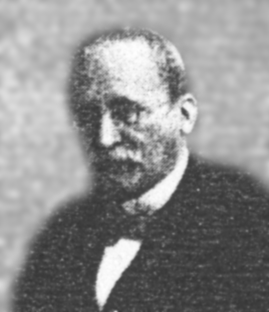
\includegraphics[width=3.886cm,height=4.531cm]{pictures/zulassungsarbeit-img010.png}

Anton Schwarz\\
\end{supertabular}
\end{flushleft}
\end{minipage}
\end{center}
{\centering

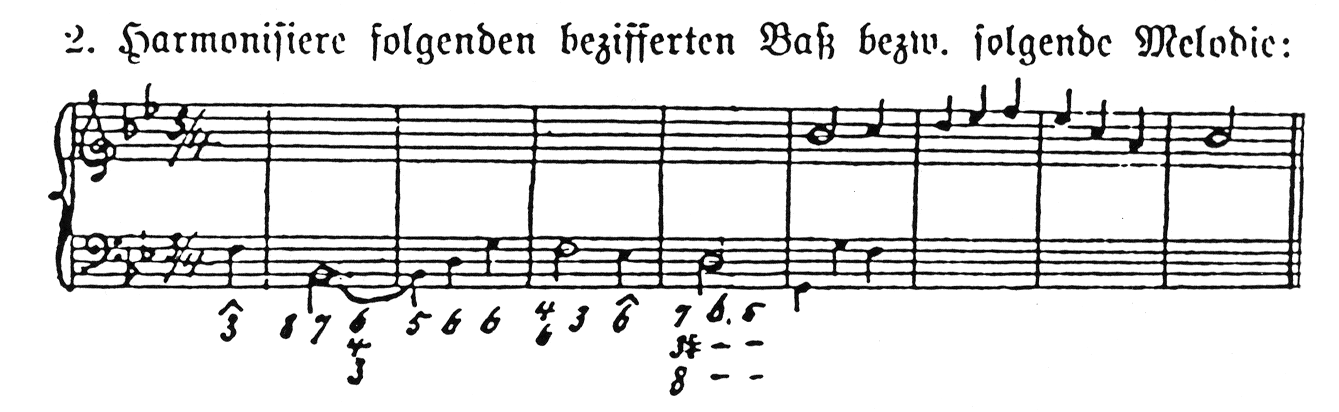
\includegraphics[width=11.088cm,height=3.258cm]{pictures/zulassungsarbeit-img011.png}
 \par}
{\centering
\label{bkm:Ref100298600}Schlussprüfung
der niederbayerischen Präparandenschulen 1903
\par}

Die Schüler erhielten zwar in ihrer Ausbildung zum Lehrer keinen
Kompositionsunterricht, dafür vermittelte ihnen der
Harmonielehreunterricht die wichtigsten tonsätzerischen Regeln, mit
denen sie in Eigenregie erste kompositorische Schritte wagen konnten.
Wie die im Fach Harmonielehre gestellten Prüfungen zeigen (Abb. 9),
gehörte das Umgehen mit dem vierstimmigen Chorsatz zu dem Handwerkszeug
eines angehenden Lehrers. Man kann deshalb August Högns Werke – sie
haben mit wenigen Ausnahmen den vierstimmigen Satz als Grundgerüst –
als Früchte des Musikunterrichts der Lehrerausbildung
betrachten. \footnote{Goller, Seite 74}

\subsection{Wanderjahre}

\hypertarget{RefHeadingToc100333728}{}Nach seinem Abschluss, dem
sogenannten „Absolutorium“, an der Lehrerbildungsanstalt in Straubing
1898, absolvierte August Högn an seiner ehemaligen Knabenschule in
Deggendorf ein Praktikum bei den Lehrern Buchner und Edelmann. Als
Aushilfslehrer waren seine Stationen Neukirchen bei Haggn im Landkreis
Straubing-Bogen, Schaufling bei Deggendorf und Geratskirchen in der
Nähe von Eggenfelden. Im Rang eines Hilfslehrers unterrichtete er in
Zeilarn bei Simbach am Inn und Wallersdorf. 1902 legte er an der
Regierung von Niederbayern die Anstellungsprüfung ab und wurde ab 1.
Januar 1903 Schulverweser in Wallersdorf. \footnote{Dokument Nr. 48,
Zeitungsartikel aus Viechtacher Bayerwald-Bote, 2.8.1958}
„Schulverweser“ ist eine 1896 eingeführte Bezeichnung für den
Schulgehilfen, also den zweiten Lehrer und Vertreter des
Schulleiters.\footnote{
http://www.markt-pfaffenhofen.de/geschichte/html\_geschichte/die\_schulverweser\_in\_pfaffenhofen.htm}
Dort lernte er seine Ehefrau Emma kennen.

\begin{figure}
\img{August-Hoegn_Wanderjahre}
\caption{August Högn}
\end{figure}

\begin{figure}
\img{Emma-Hoegn}
\caption{Emma Högn}
\end{figure}

\begin{figure}
\img{Hochzeitseinladung-und-Menue}
\caption{Hochzeitseinladung und Menü}
\end{figure}

Am 20. Juli 1904 fand in Wallersdorf die Hochzeit von August Högn und
der neun Jahre jüngern, damals 16-jährigen Emma Gerstl mit üppigem
Hochzeitsmenü statt, wie der Hochzeitseinladung (Abb. 12) entnommen
werden kann. \footnote{Dokument Nr. 111, Einladung zur Hochzeitsfeier,
20.7.1904} Emma Gerstl stammte aus einer wohlhabenden\footnote{
Interview Nr. 4, Maria Schröck, 30.12.2002, Absatz 4}
Bierbrauerfamilie,die in Gründobl, einem
kleinen Ort in der Nähe von Wallersdorf, ein großes Anwesen mit
Brauerei \footnote{Interview Nr. 21, Lilo Leuze, 2.12.2004, Absatz 20}
und Wirtshaus \footnote{Interview Nr. 3, Ida Högn, 29.12.2002, Absatz
36} besaß. Das junge Paar musste heiraten, da Emma Högn schwanger
wurde. Sie gebar Zwillinge, die beide kurz nach ihrer Geburt
starben. \footnote{Interview Nr. 3, Ida Högn, 29.12.2002, Absatz 36;
Interview Nr. 25, Lilo Leuze, 14.1.2005, Absatz 2} Zum 1. Juni 1905
wurde Högn nach Eberhardsreuth im Landkreis Grafenau
versetzt. \footnote{Dokument Nr. 48, Zeitungsartikel aus Viechtacher
Bayerwald-Bote, 2.8.1958} Hier kam die Tochter Elfriede, genannte
Frieda, am 14. August 1906 zur Welt. \footnote{Interview Nr. 20,
Gertraud von Molo, 23.11.2004, Absatz 6} Der Sohn Gustl erblickte am
17.1.1912 schon in Högns nächstem Einsatzort das Licht der Welt: in
Ruhmannsfelden. \footnote{Taufregister der Pfarrgemeinde St.
Laurentius, Ruhmannsfelden}

\begin{figure}
\img{Gustl-und-Frieda-Hoegn}
\caption{Gustl und Frieda Högn}
\end{figure}

\subsection{Schnelle Integration in Ruhmannsfelden}

August Högn wurde zum 1.1.1910 an
die Volksschule in Ruhmannsfelden versetzt. \footnote{Dokument Nr. 48,
Zeitungsartikel aus Viechtacher Bayerwald-Bote, 2.8.1958} Der Markt
Ruhmannsfelden, in dem damals ungefähr 1500 Einwohner lebten, liegt im
bayerischen Wald und ist etwa in der Mitte des Dreiecks zu finden, das
die nächst gelegenen drei Städte Viechtach, Regen und Deggendorf
bilden. \footnote{Högn, Ruhmannsfelden, S. 50} Das Einzugsgebiet der
Volksschule umfasste auch vor dem 1. Weltkrieg nicht nur die Gemeinde
Ruhmannsfelden, sondern zusätzlich weite Teile der benachbarten
Gemeinde Zachenberg und Randgebiete der angrenzenden Gemeinde
Patersdorf, also in etwa das Gebiet der Pfarrei St. Laurentius. Die
Gemeinde Zachenberg, die geringfügig mehr Einwohner als Ruhmannsfelden
zählte, bestand aus 38 überwiegend landwirtschaftlich geprägten
Kleinstortschaften und hatte mit dem Dorf Zachenberg kein wirkliches
Zentrum, denn dort bestand weder ein Rathaus noch ein Schulhaus. Nicht
nur in Schulangelegenheiten war Ruhmannsfelden damals wie auch heute
ein Zentrum. Ansässige Ärzte und eine seit 1910 bestehende
Apotheke \footnote{Högn, Ruhmannsfelden, S. 28 – 29} lieferten auch für
die Bewohner der Nachbargemeinden Achslach und Gotteszell einen Grund,
Ruhmannsfelden zu besuchen.

\begin{figure}
\img{Ruhmannsfelden}
\caption{Ruhmannsfelden zur Zeit August Högns}
\end{figure}

Man kann davon ausgehen, dass Högn Ruhmannsfelden als einen
fortschrittlichen Ort erlebt hat, da dort kurz vor seiner Ankunft
Investitionen getätigt und Reformen durchgeführt wurden. So besaß
Ruhmannsfelden seit dem Schulhausneubau im Jahr 1908 (Abb. 16) gleich
drei Schulhäuser. \footnote{Reicheneder-Chronik, Schulwesen, Blatt 76
Vorderseite} Das älteste, 1834 erbaute Schulhaus (Abb. 15) konnte als
Lehrerwohnhaus genutzt werden und bot somit der jungen Familie eine
Wohnmöglichkeit. \footnote{Reicheneder-Chronik, Schulwesen, Blatt 68
Vorderseite} Auch in institutioneller Hinsicht hatte sich an der
Volksschule Ruhmannsfelden kurz vor 1910 Einiges geändert. Dem
Anwachsen der Schülerzahl wurde Rechnung getragen und statt früher vier
unterrichten nun sieben Lehrer, also ein Lehrer pro Schülerjahrgang.
Den jahrgangsübergreifenden und nach Geschlechtern getrennten Klassen
war somit ein Ende gesetzt. Die gemischten Jahrgänge umfassten aber
immer noch fast durchschnittlich 70 Schüler.\footnote{
Reicheneder-Chronik, Schulwesen, Blatt 16 Rückseite} 1908 hatten die
Anträge der Gemeinden Zachenberg und Patersdorf auf Einführung einer
Sommerschule Erfolg. Damit Kinder vor allem zur Erntezeit in der
Landwirtschaft ihrer Eltern mithelfen konnten, wurde vom 1. Mai bis 1.
Oktober ein auf drei Stunden verkürzter Unterricht
eingeführt. \footnote{Reicheneder-Chronik, Schulwesen, Blatt 8
Vorderseite}

\begin{figure}
%
\begin{subfigure}[t]{0.3\linewidth}
\centering
\img[height=3cm]{Schulhaus-1834}
\caption{Schulhaus von 1834, ab 1908 als Lehrerwohnhaus genutzt}
\end{subfigure}
%
\begin{subfigure}[t]{0.7\linewidth}
\centering
\hfil\img[height=3cm]{Schulhaus-1908}
\caption{Schulhaus von 1908}
\end{subfigure}
%
\caption{Die Ruhmannsfeldener Schulhäuser}
\end{figure}

Mit August Högn traten gleich drei neue Lehrer in Ruhmannsfelden ihren
Schuldienst an. In der Schulchronik wird Högn bald als 2. Lehrer und
somit Stellvertreter von Schulleiter Alois Auer aufgeführt.\footnote{
Volksschul-Chronik} Das hatte neben seiner schon 10 Jahre langen
Berufserfahrung wahrscheinlich auch den Grund, dass Högn die einzige
männliche Lehrerkraft neben Bezirksoberlehrer Auer war, die in den
unruhigen Zeiten des 1. Weltkrieges seiner neuen Heimat treu bleiben
konnte. Högns Kriegseinsatz beschränkte sich auf einen kurzen
Heeresdienst im Jahr 1915, bei dem er sich den König-Ludwig-Orden und
das Militär-Verdienstkreuz erwarb.

Eine weitere Neuerung war, dass die Pfarrkirche St. Laurentius im selben
Jahr, als August Högn nach Ruhmannsfelden kam, eine neue, pneumatische
Orgel mit 22 Registern vom Orgelbaumeister Ludwig Edenhofer aus
Deggendorf bekam. \footnote{Reicheneder-Chronik, Orgel, Blatt 74
Rückseite} Von Anfang an wirkte Högn an der Kirchenmusik in
Ruhmannsfelden mit. \footnote{Dokument Nr. 18, Brief von August Högn an
Pfarrer Reicheneder, 25.1.1954} Der versierte Orgelspieler\footnote{
Interview Nr. 16, Maria Freisinger, 25.8.2004, Absatz 28} war auch im
Kirchendienst mehr als ein würdiger Stellvertreter für Auer, der
zusammen mit seiner Frau Anna und Tochter Auguste den
Chorregentendienst ausführte.

Bereits ein halbes Jahr nach seiner Ankunft wurde Högn zum Vorstand
eines Ruhmannsfeldener Vereins gewählt, was seine schnelle
gesellschaftliche Integration in Ruhmannsfelden unterstreicht. Der
Turnverein Ruhmannsfelden suchte zu dem Zeitpunkt händeringend eine
Person, die sich bereit erklärte, den unbesetzten Posten des Vorstands
zu übernehmen. Vom 21.5.1910 \footnote{Dokument Nr. 101, Protokoll der
Turnvereinsversammlung, 21.5.1910}  bis 27.12.1913 \footnote{Dokument
Nr. 103, Protokoll der Turnvereinsversammlung, 27.12.1913} hatte Högn
dieses Amt inne. Auch wenn er nach dieser Zeit in keiner Funktion der
Vereinsspitze in Erscheinung tritt, blieb er trotzdem über Jahrzehnte
hinweg vor allem als Leiter der Sänger- und Orchesterriege dem Verein
treu. 1924 versuchte man noch einmal Högn in die Vereinsspitze als
Schriftführer mit einzubinden, doch er lehnte wahrscheinlich deswegen
ab, weil er schon bei der Ruhmannsfeldener Feuerwehr die
Schriftführertätigkeit ausübte. \footnote{Dokument Nr. 107, Protokoll
der Turnvereinsversammlung, 23.1.1924}

August Högn war bereits am 19.9.1902 der Wallersdorfer Feuerwehr
beigetreten \footnote{Dokument Nr. 110, Abschiedsrede des
Feuerwehrkommandanten Johann Linsmeier auf August Högn, 3.11.1951} und
wechselte Anfang Januar 1910 in die Feuerwehr Ruhmannsfelden. Am
26.12.1910 wurde Högn dann zum Schriftführer der Feuerwehr
Ruhmannsfelden gewählt. \footnote{Dokument Nr. 93, Protokoll der
Feuerwehrgeneralversammlung, 26.12.1910} Dass ein Lehrer den
Schriftführerposten der Feuerwehr übernahm, hatte in Ruhmannsfelden
Tradition. Die Lehrer Raymund Schinagl und Max Weig waren lange Zeit
vor Högn als Schriftführer tätig. Der Feuerwehr-Mitbegründer und letzte
Schriftführer Joseph Lukas starb am 30.8.1910, \footnote{Högn,
Feuerwehr, Blatt 7 b, Blatt 17, Blatt 34} sodass sein Posten frei
wurde. August Högn, als Lehrer im Schreiben souverän wie sonst kein
anderer bei der Feuerwehr, bot sich als Nachfolger für Lukas gerade zu
an. Die Protokolle vor Högns Zeit als Schriftführer zeichnen sich
dementsprechend durch viele Rechtschreibfehler aus.\footnote{
Feuerwehr-Protokoll} August Högn blieb 40 Jahre lang Schriftführer der
Feuerwehr. Neben dem Verfassen von Protokollen übernahm er die
Korrespondenz der Feuerwehr, hielt zahlreiche Ansprachen und Vorträge
und packte auch mal mit eigenen Händen an, als zum Beispiel 1933 bei
strömenden Regen die neue Feuerwehrspritze vom Zug abgeladen werden
musste. \footnote{Högn, Feuerwehr, Blatt 44, Blatt 46, Blatt 47, Blatt
54, Blatt 56}

Ein weiteres Aufgabenfeld, das die damalige dörfliche Gemeinschaft für
einen Lehrer bereithielt, übernahm August Högn 1913: Bis 1920 war August
Högn Gemeindeschreiber der Gemeinde Zachenberg. \footnote{Högn,
Zachenberg, Blatt 16} Nach dem Erlass der Gemeindeverordnung wurden
diese Arbeiten hauptsächlich den Lehrern übertragen. \footnote{Geyer,
Seite 106} So verwundert es nicht, dass die angehenden Lehrer in den
Lehrerbildungsanstalten speziell im Fach Gemeindeschreiberei
unterrichtet wurden \footnote{Dantl, Seite 82} und dass vor Högn die
Lehrer Milter, Schinagl, Lechner und Hochstraßer für die Gemeinde
Zachenberg tätig waren. \footnote{Högn, Zachenberg, Blatt 11, Blatt 15,
Blatt 16} Högns Eifer, sich für das Gemeinwohl zu engagieren, kommt auch
dadurch besonders zum Ausdruck, dass er sogar ein Zimmer seiner
Dienstwohnung abtrat und es in eine Art Gemeindekanzlei umwandelte.
Vorher wurden die Gemeindearbeiten, die für Lehrer eine wichtige
Nebeneinkunft darstellten, in einem Raum der Brauerei Rankl in
Ruhmannsfelden erledigt.

\subsection{Leiter des Turnverein-Orchesters}

Ähnlich wie andere Vereine am Ort, veranstaltete der Turnverein
Ruhmannsfelden bunte Abende oder führte Theaterstücke, Singspiele und
sogar Operetten auf und übernahm somit weit über die eigentliche
Vereinsaufgabe hinaus eine wichtige kulturelle Funktion.
\footnote{Dokument Nr. 56, Auszug aus den Memoiren von Franz Danziger
sen., 1984} Zumindest für den Turnverein war die Veranstaltung
derartiger Unterhaltungsprogramme eine bedeutende Einnahmequelle für die
Finanzierung geplanter Projekte wie beispielsweise den Turnhallenbau. Es
ist daher keineswegs verwunderlich, dass sich für August Högn in den
Anfangsjahren in Ruhmannsfelden insbesondere unter dem Dach des
Turnvereins ein musikalisches Betätigungsfeld auftat, obwohl die
ursprüngliche Aufgabe des Vereins nichts mit Musik zu tun hatte. Der
ehemalige Vorstand unterstützte den Verein nun als Leiter einer Sänger-
und Orchesterriege. \footnote{Dokument Nr. 98, Geschichtliches über die
Erbauung der Turnhalle in Ruhmannsfelden, 1928}

Am 27.9.1919 wurde die Sängerriege im Turnverein gegründet. Als erster
Leiter erscheint zwar Rudolf Schwannberger, Nachbar von Högn und
Kirchenchorsänger. \footnote{Dokument Nr. 104, Protokoll der
Turnvereinsversammlung, 27.9.1919} Doch laut des Turnverein-Protokolls
fungierte Högn bereits ab 29.12.1919 als Dirigent. \footnote{Dokument
Nr. 105, Protokoll der Turnvereinsversammlung, 29.12.1919} 1921 wird
Schwannberger als Gesangswart und Högn als Gesangsdirigent der
Sängerriege bezeichnet, \footnote{Dokument Nr. 106, Protokoll der
Turnvereinsversammlung, 10.12.1921} die sich im Saal der Brauerei
Vornehm zum Proben traf. Über die Orchesterriege, die im Haus des
Apothekers Voit probte, sind im Vereinsprotokoll keine Eintragungen zu
finden. Wahrscheinlich kam das Streichorchester nur dann zusammen, wenn
ein Stück eine Instrumentalbegleitung der Sänger benötigte.

\begin{figure}
%
\begin{subfigure}[t]{0.5\linewidth}
\centering
\img[height=7cm]{Rudolf-Schwannberger}
\caption{Rudolf Schwannberger}
\end{subfigure}
%
\begin{subfigure}[t]{0.5\linewidth}
\centering
\img[height=7cm]{August-Hoegn_Turnverein}
\caption{August Högn}
\end{subfigure}
%
\caption{Der Gesangswart und der Gesangsdirigent der Sängerriege}
\end{figure}

Leider ist nur wenig über die Veranstaltungen im Einzelnen bekannt. Es
ist nicht bekannt, wie regelmäßig sie stattfanden und in welchem
Zeitraum der Turnverein sich derart kulturell engagierte. Einen kleinen
Einblick in das damalige kulturelle Leben gewährt uns aber, die nicht
nur in finanzieller Hinsicht erfolgreichste „Produktion“ des
Turnvereins: die Aufführungen des Singspiels „Der Holledauer Fidel“ von
Erhard Kutschenreuter im Jahr 1923. \footnote{Dokument Nr. 98,
Geschichtliches über die Erbauung der Turnhalle in Ruhmannsfelden,
1928} Dieses Singspiel forderte eine große Anzahl an Mitwirkenden. Im
dritten Akt ist beispielsweise ein Trachtenfestzug verlangt, der über
die Bühne zieht. \footnote{Proft, Seite 58} Große Anforderungen an die
Gesangeskünste der Mitwirkenden stellten die vielen Gesangsnummer des
Singspiels, wie etwa das Liebeslied des Fidel, das Duett des Sichbauern
und dessen Frau, das Lied der Reserl, ein Kinderchor und die großen
Chorszenen zu Beginn und zum Schluss des Singspiels. \footnote{Proft,
Seite 57} Instrumentalstücke, wie zum Beispiel das polyphon angelegt
Vorspiel zum zweiten Akt \footnote{Proft, Seite 55} der
„Holledauer-Marsch“ und der „Waldler-Marsch“, \footnote{Proft, Seite
57} stellten eine Herausforderung für das Turnverein-Orchester dar, das
aus drei Violinen und einer Viola, einem Violoncello und einem
Kontrabass, also sechs Musikern, ähnlich wie das Kirchenorchester,
bestand.

\begin{figure}
\img{Holledauer-Fidel}
\caption{Die Mitwirkenden der Aufführungen des Singsspiels „Der
Holledauer Fidel“}
\end{figure}

Die ca. 60 an den 8 Aufführungen des Singsspiels „Der Holledauer Fidel“
von Erhard Kutschenreuter im März 1923 beteiligten Personen. In der
Mitte (Pfeile) sind August Högn und seine Tochter Frieda zu sehen.

Diese ungewöhnlich große Anzahl an Mitwirkenden – auf dem Foto (Abb. 19)
sind 60 Personen zu sehen – machte es notwendig, dass die Bühne im
Vornehmsaal ausnahmsweise an der Längsseite aufgestellt werden musste,
sodass die Akteure nur direkt vom Freien aus auf die Bühne gelangen
konnten. \footnote{Dokument Nr. 98, Geschichtliches über die Erbauung
der Turnhalle in Ruhmannsfelden, 1928} Die große Teilnehmerzahl ist auf
die Unterstützung weiterer Vereine zurückzuführen, insbesondere jedoch
des Kirchenchores und der Lehrerschaft. August Högn, der die gesamte
musikalische Leitung übernommen hatte und als Dirigent fungierte, war
in seiner Eigenschaft als Chorregent und Schulleiter der ideale Mann,
weitere geeignete Mitwirkende für das Singspiel zu gewinnen.

Die Einkünfte der acht im Saal der Brauerei Vornehm stattgefundenen und
ausverkauften Aufführungen des Singspiels erbrachten einen Gewinn von
500 M, mit dem ein Grundstück erworben werden konnte, das als Turnplatz
verwendet wurde. \footnote{Dokument Nr. 95, Programmzettel zur
Aufführung des Singspiels {\textquotedbl}Der Holledauer
Fidel{\textquotedbl}, Mrz. 1923} Dieser durchschlagende Erfolg der
Aufführungen des „Fidels“ – sie verhalfen dem Turnverein sogar zu einem
eigenen Turnplatz – ist auch auf das Stück zurückzuführen. Mit dem
„Fidel“ hatte der im Rottal ansässige Lehrer Erhard Kutschenreuter mit
Abstand sein erfolgreichstes Stück geschrieben. \footnote{Proft, Seite
53} Nach der Uraufführung in Passau im Jahr 1920 erlebte das Singspiel
schon 1938 die 3000. Aufführung. \footnote{Proft, Seite 60} Die
Ruhmannsfeldener Zuschauer strömten vielleicht auch deswegen so
zahlreich in die Vorstellungen weil die Handlung des Stückes zum Teil
im bayerischen Wald spielt: Der arme Hopfenzupfer Fidel Waldhauser aus
dem bayerischen Wald verliebt sich in die Tochter des reichen
Sichbauern aus der Hallertau, gespielt von August Högns Tochter
Frieda. \footnote{Dokument Nr. 95, Programmzettel zur Aufführung des
Singspiels {\textquotedbl}Der Holledauer Fidel{\textquotedbl}, Mrz.
1923} Trotz auftretender Hindernisse, die unüberwindbar zu sein
scheinen, findet das ungleiche Paar schließlich doch zusammen, und es
kommt zur Hochzeit. Den Zuschauern in Ruhmannsfelden waren die
dargestellten sozialen Verhältnisse sicher gut bekannt, denn viele von
ihnen fuhren selbst, wie es bis in den fünfziger Jahren des letzten
Jahrhundert üblich war, einmal jährlich in die Hallertau zur
Hopfenernte, um ein Zusatzeinkommen zu verdienen. \footnote{Proft,
Seite 56}

\begin{figure}
\img{Programm_Holledauer-Fidel}
\caption{Programm zu den „Fidel“-Aufführungen}
\end{figure}

Am 21. Juli 1923 wurde August Högn von der Gemeinde Ruhmannsfelden das
Ehrenbürgerrecht \zitat{„aus Anlass seines 25-jährigen Dienstjubiläums“}
\footnote{Reicheneder-Chronik, Ehrenbürger, Blatt 1 Vorderseite} und
\zitat{„für die großen Verdienste, die er sich um Schule und Gemeinde
erwarb“} \footnote{Reicheneder-Chronik, Ehrenbürger, Blatt 1
Vorderseite} verliehen. Dieser Titel stellte damals schon eine besondere
Auszeichnung dar und wurde daher nur an wenige sich außerordentlich
verdient gemachte Bürger verliehen. Die Ehrenbürgerurkunde bekamen
außerdem Pfarrer Mühlbauer (1906) sowie August Högns Vorgänger als
Schulleiter Alois Auer (1910). Nach Högn wurde sie 1933 an Adolf Hitler
verliehen. \footnote{Reicheneder-Chronik, Ehrenbürger, Blatt 1
Vorderseite} Die Aufführungen des „Holledauer Fidels“ etwas länger als
ein Vierteljahr davor, lassen den Anlass für die Ehrenbürgerrechts-
Verleihung Högns in ganz anderem Licht erscheinen. Ist es nicht
offensichtlich, dass die Singspielabende, an denen Högn in
hervorragender Weise mitgearbeitet hatte und die dem Turnverein zum
Erwerb eines Turnplatzes verhalfen, eher als der Hauptgrund für die
Verleihung anzusehen ist, als sein 25. Dienstjubiläum, das wohl eher
einen weiterem Grund darstellt?

Aus finanzieller Sicht war der Turnverein am Bau seiner eigenen
Turnhalle mit einem großen Betrag beteiligt. Die Einkünfte vieler
bunter Abende sowie weitere Theateraufführungen, wie z. B. die
Aufführung der Operette „Der Postillion“  \footnote{Dokument Nr. 56,
Auszug aus den Memoiren von Franz Danziger sen., 1984} von Ludwig
Eckl, \footnote{Goller, Seite 188} dürften direkt in den Turnhallenbau
geflossen sein. Högn engagierte sich nicht nur musikalisch für die
Anliegen des Turnvereins, sondern auch politisch. 1925 begrüßte er eine
Kommission des bayerischen Landtages in Ruhmannsfelden und äußerte
ihnen unter anderem die Bitte um Bezuschussung des Turnhallenbaus. Am
29. Januar 1928 wurde die Ruhmannsfeldener Turnhalle schließlich
eingeweiht und ein \zitat{„großers Orchester aus lauter
Ruhmannsfeldener Musikern“} \footnote{Dokument Nr. 98, Geschichtliches
über die Erbauung der Turnhalle in Ruhmannsfelden, 1928} spielte zur
Feier des Tages.

\begin{figure}
\img{Turnhalle}
\caption{Turnhalle des Turnvereins Ruhmannsfelden}
\end{figure}

\subsection{Alte und neue Familie}
\hypertarget{RefHeadingToc100333731}{}Völlig überraschend starb am 19.
Juni 1926 August Högns Ehefrau Emma im Alter von 39 Jahren\footnote{
Dokument Nr. 109, Traueranzeige von August Högns Ehefrau Emma,
19.6.1926} an einem Gallendurchbruch. \footnote{Interview Nr. 20,
Gertraud von Molo, 23.11.2004, Absatz 4} Mitten aus dem Leben gerissen
hinterließ Emma Högn, die kurze Zeit davor Großmutter geworden war,
einen erst 14 Jahre alten Sohn. Das Tragische an Emmas Tod war, dass
sie an einer Krankheit starb, die schon zur damaligen Zeit hätte
behandelt werden können, wären die Symptome frühzeitig erkannt worden.
Mit nur 47 Jahren war August Högn Witwer geworden und musste sich nun
alleine um die Erziehung seines minderjährigen Sohns Gustl kümmern. Zur
Verrichtung der alltäglichen Arbeiten wurde auch deshalb die
Haushälterin Rosa Beischmied angestellt. \footnote{Interview Nr. 2,
Barbara Essigmann, 27.12.2002, Absatz 98}

\begin{center}
\begin{minipage}{5.992cm}
\begin{center}
\tablefirsthead{}
\tablehead{}
\tabletail{}
\tablelasttail{}
\begin{supertabular}{m{5.7920003cm}}

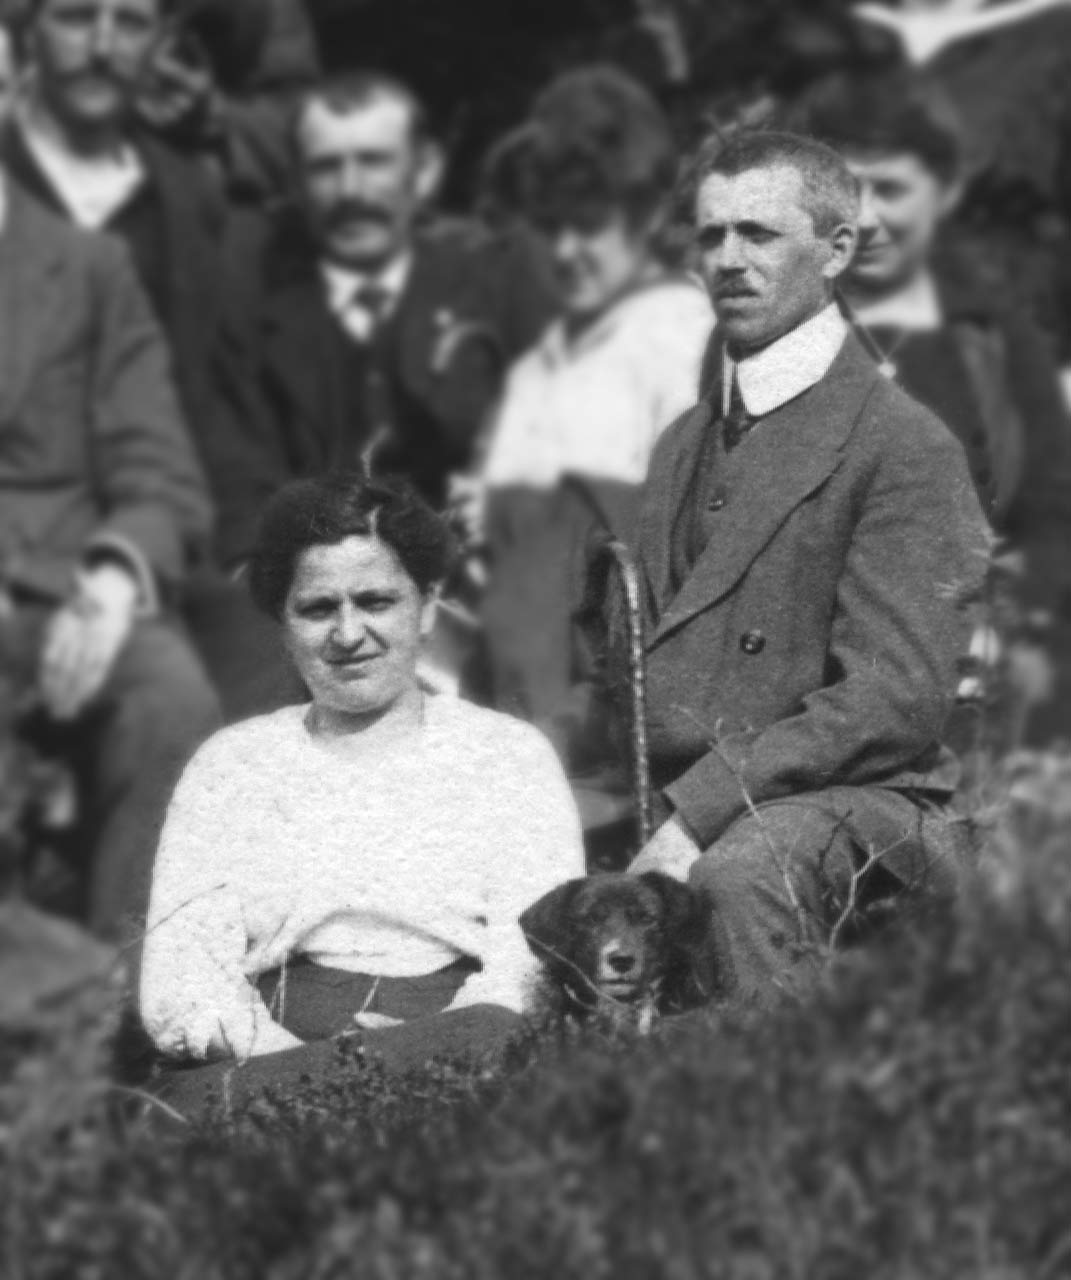
\includegraphics[width=5.609cm,height=6.705cm]{pictures/zulassungsarbeit-img024.jpg}

Emma und August Högn mit Jagdhund
„Treff“ bei einer Wanderung.\\
\end{supertabular}
\end{center}
\end{minipage}
\end{center}
Über den Zustand der Ehe Högns mit Emma ist kaum etwas bekannt.
Gerüchten zufolge soll Högns Ehefrau eine Affäre mit dem Nachbarn und
Kirchenchorsänger Rudolf Schwannberger gehabt haben.\footnote{
Interview Nr. 3, Ida Högn, 29.12.2002, Absatz 10} Ein möglicher Grund,
weshalb Högn kein zweites Mal geheiratet hat, könnte seine große Liebe
zu Emma gewesen sein. Ein weiterer Grund dafür dürfte auch seine
partnerschaftliche Beziehung zu Rosa Beischmied dargestellt haben, die
sich unweigerlich im Laufe der Jahre entwickelt hatte. Beide wurden als
eingespieltes Team beschrieben. \footnote{Interview Nr. 3, Ida Högn,
29.12.2002, Absatz 10} 35 Jahre lang begleitete Rosa Beischmied August
Högn bis zu seinem Tod und lebte mit ihm gemeinsam in derselben
Wohnung. \footnote{Interview Nr. 21, Lilo Leuze, 2.12.2004, Absatz 10;
Interview Nr. 20, Gertraud von Molo, 23.11.2004, Absatz 12} Je nach
Lebenslage unterstützte ihn die „Högn Rosl“, wie sie von einigen
Zeitzeugen genannt wurde, \footnote{Interview Nr. 2, Barbara Essigmann,
27.12.2002, Absatz 10, 76} etwa bei der Erziehung seines Sohnes, aber
auch beim Schuldienst, wenn zum Beispiel Högns Schüler Vitamintabletten
auf seine Anordnung hin, bei Rosa abholen mussten. \footnote{Interview
Nr. 6, Wilhelm Ederer, 2.1.2003, Absatz 34} Aber auch im Alter wurde
Högn von Rosa gepflegt, besonders nach seinem Schlaganfall.\footnote{
Dokument Nr. 73, Brief von August Högn an Stephan Leitner, 10.3.1961}
Nicht selbstverständlich und daher ebenso ein Indiz für das doch über
das rein Dienstliche hinausgehende Verhältnis zwischen Högn und
Beschmied war die Tatsache, dass Rosa Beischmieds „illegale“ Tochter
Mathilde, wie im Taufregister zu lesen ist, nach dem Tod ihrer
Großeltern in Högns Wohnung einziehen durfte. In der großen Wohnung im
Schulhaus erhielt sie ein eigenes Zimmer \footnote{Interview Nr. 19,
Mathilde Beischmied, 14.9.2004, Absatz 22} und fühlte sich von August
Högn sogar soweit akzeptiert, dass sie ihn heute als „Ersatzvater“
bezeichnet. \footnote{Interview Nr. 19, Mathilde Beischmied, 14.9.2004,
Absatz 18} Eine Anekdote, die Mathilde Beischmied in einem Interview
erzählte, mag vielleicht exemplarisch das gute und sehr
freundschaftliche Verhältnis Högns zu seiner Ziehtochter beleuchten und
Einblick ins damalige „Familienleben“ geben: Als Belohnung dafür, dass
die kleine Mathilde für Högn das Bier holte, bestand Högn darauf, dass
auch sie etwas von dem besorgten Getränk abbekam und fragte deshalb
ihre Mutter vorwurfsvoll: \zitat{„Kriegt sie heute kein
Bier?“ } \footnote{Interview Nr. 19, Mathilde Beischmied, 14.9.2004,
Absatz 6} Auch in der Funktion des Vaters, obwohl diese Bezeichnung
nicht zutrifft, zeigte sich Högn, als er für mehrere Jahre seine noch
schulpflichtige Enkelin Inge bei sich aufnahm. Als Grund, weshalb sie
zu ihrem Großvater kam, kann wohl die Trennung der ihrer Mutter Frieda
von ihrem ersten Ehemann und die neue Bekanntschaft mit ihrem späteren
Ehemann Dr. Karl Schlumprecht angesehen werden. \footnote{Interview Nr.
19, Mathilde Beischmied, 14.9.2004, Absatz 26} Da auch Högns Sohn Gustl
noch zu Hause wohnte, zählte Högns „neue Familie“ zusammen mit der
Enkelin Inge zeitweise sogar fünf Mitglieder.

\subsection{Chorregentendienst mit Unterbrechung}

Zum 1. September 1921 wurde, dem
Protokoll der Kirchenverwaltungssitzung zufolge, August Högn der
Chorregenten- und Organistendienst provisorisch übertragen.\footnote{
Dokument Nr. 116, Protokoll der Kirchenverwaltungssitzung, 21.8.1921}
Provisorisch steht hier nur deshalb, weil ein Jahr zuvor die gesetzlich
geregelte Verbindung zwischen Schul- und Kirchendienst, die mittels der
Chorregenten-, Organisten- und Mesnertätigkeiten der Lehrer bestand,
abgeschafft worden war. Besonders am Vormittag stattfindende
Beerdigungen standen der längerfristigen Weiterführung des
Organistendienst durch die Lehrer im Weg. Da viele Lehrer sich
freiwillig bereit erklärten, weiterhin Chorregent zu bleiben, ließ sich
diese jahrhunderte alte Tradition nicht von heute auf morgen
abschaffen. Den Schulbehörden blieb anscheinend nichts anderes übrig,
als den Chorregentendienst der Lehrer, verbunden mit den
Stundenausfällen, zumindest für eine gewisse Übergangszeit zu dulden.

\begin{center}
\begin{minipage}{9.491cm}
\begin{flushleft}
\tablefirsthead{}
\tablehead{}
\tabletail{}
\tablelasttail{}
\begin{supertabular}{m{4.8960004cm}m{4.196cm}}

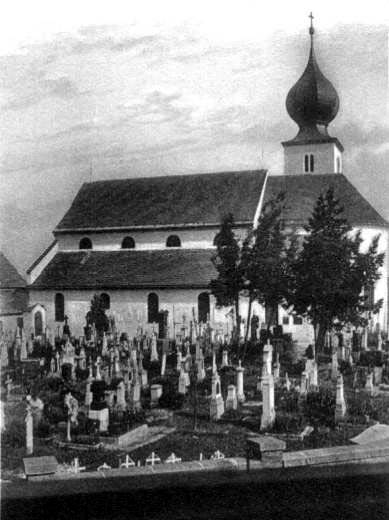
\includegraphics[width=4.713cm,height=6.301cm]{pictures/zulassungsarbeit-img025.jpg}

Pfarrkirche St. Laurentius zur Zeit von
August Högn &

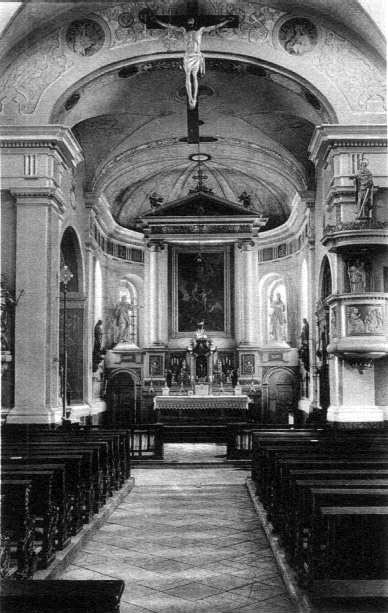
\includegraphics[width=4.013cm,height=6.292cm]{pictures/zulassungsarbeit-img026.jpg}

Blick zum Altarraum\\
\end{supertabular}
\end{flushleft}
\end{minipage}
\end{center}
Eine weitere Tradition, nämlich dass der Schulleiter den
Chorregentendienst übernahm, \footnote{Dokument Nr. 55, Artikel in der
Reicheneder-Chronik über August Högn} wurde in Ruhmannsfelden
fortgeführt, obwohl der Kirchendienst der Lehrer offiziell abgeschafft
wurde, als August Högn nach der Pensionierung des Bezirkshauptlehrers
Alois Auer 1921 \footnote{Reicheneder-Chronik, Pfarrmesner, Blatt 1
Vorderseite} nicht nur Chorregent, sondern
auch Schulleiter wurde. Max Weig war von 1879 bis zu seinem Tod 1895
Schulleiter und somit auch Organist und Chorregent.\footnote{
Reicheneder-Chronik, Schulwesen, Blatt 100
Rückseite}Erst im seinem Todesjahr kam vom
königlichen Bezirksamt Viechtach die Anweisung, dass ein Hilfslehrer
den Chorregentendienst übernehmen sollte. \footnote{Dokument Nr. 1,
Brief von Bezirkshauptmann Heerwagen an Kirchenverwaltung, 18.1.1895}
Von 1895 bis 1921 \footnote{Reicheneder-Chronik, Schulwesen, Blatt 110
Vorderseite} leitete Weigs Nachfolger, der Schulleiter Alois Auer,
zusammen mit seiner Frau Anna den Chor, ehe Högn ihn
fortführte. \footnote{Dokument Nr. 6, Brief von Max Rauscher sen. an
Kirchenverwaltung, 14.3.1927}

Vor allem aber dürften seine überdurchschnittlichen musikalischen
Fähigkeiten Högn dazu bestimmt haben, die alte Tradition des Lehrers
und Chorregenten in Personalunion weiterzuführen. Bevor er die
Kirchenchorleitung übernahm, hatte er über 20 lang Jahre als
guter \footnote{Dokument Nr. 48, Zeitungsartikel aus Viechtacher
Bayerwald-Bote, 2.8.1958} Tenor \footnote{Interview Nr. 5, Barbara
Essigmann, 2.1.2003, Absatz 40} und versierter Organist – man sagte von
ihm, dass er gleichzeitig singen, spielen und dirigieren
konnte \footnote{Interview Nr. 16, Maria Freisinger, 25.8.2004, Absatz
28} – in verschiedenen Orten an der Kirchenmusik mitgewirkt und
Erfahrungen gesammelt. \footnote{Dokument Nr. 18, Brief von August Högn
an Pfarrer Reicheneder, 25.1.1954} Nicht nur im Manualspiel war er
gewandt, wie die virtuos gesetzte Fassung seines Marsches „In Treue
fest!“ für Klavier zu zwei Händen beweist, sondern auch mit dem
Pedaleinsatz konnte er von seinem Können überzeugen.\footnote{
Interview Nr. 4, Maria Schröck, 30.12.2002, Absatz 58} Unter seinen
Stücken, die er auf der Orgel spielte, war die berühmte und nicht
gerade leicht zu spielende Toccata und Fuge in d-moll von Johann
Sebastian Bach. Angesichts einer derart gehoben Orgelliteratur, die zu
seinem Repertoire gehörte, überrascht es daher nicht, wenn manche
Kirchenbesucher so lange in der Kirche blieben, um Högns Orgelspiel bis
zum Schluss beiwohnen zu. \footnote{Interview Nr. 11, Josef Stern,
21.2.2003, Absatz 2} Nicht zu vergessen sind auch seine
kompositorischen Fähigkeiten: Innerhalb von wenigen Tagen konnte er für
den Einsatz in der Kirchenmusik passende Kompositionen schreiben. Ein
befreundeter Chorleiter bat Högn in einem Brief, ein Stück für seinen
Männerchor zu schreiben. \footnote{Dokument Nr. 62, Brief von „Franzl“,
Regen an August Högn, 17.6.1928} Laut einem Vermerk auf der
betreffenden Komposition wurde das Stück schon zwei Tage später fertig
gestellt. Kein Wunder also, dass seine musikalischen Leistungen auch im
Urteil seiner Zeitgenossen lobende Anerkennung fanden. Bischof
Buchberger zum Beispiel hob bei einer Firmung hervor, dass er selten
einen so guten Organisten Orgel spielen gehört habe.\footnote{
Interview Nr. 13, Lorenz Schlagintweit, 29.11.2003, Absatz 2} Josef
Brunner, der als Organist an der Kirchenmusik unter Högn mitwirkte,
meinte sogar: \zitat{„Der Högn war ein selten guter Musiker.
So einer steht nicht mehr auf.“ } \footnote{Interview Nr. 8, Josef
Brunner, 3.1.2003, Absatz 16}

\zitat{„Zur größten Zufriedenheit der ganzen Kirchengemeinde“}
\footnote{Dokument Nr. 12, Brief von Kirchenverwaltung an Regierung
von Niederbayern, 1.4.1927} leitete August Högn laut Pfarrer Fahrmeier
den Kirchenchor bis Ende 1924 und ein Ruhmannsfeldener Bürger, der die
Entwicklung des Kirchenchors über einen längeren Zeitraum beurteilen
konnte, bestätigte, dass der Chor, der unter dem Lehrer Weig
\zitat{„einen guten Namen hatte,“ } \footnote{Dokument Nr. 6,
Brief von Max Rauscher sen. an Kirchenverwaltung, 14.3.1927} und unter
der Leitung von Anna Auer \zitat{„einen Niedergang“
} \footnote{Dokument Nr. 6, Brief von Max Rauscher sen. an
Kirchenverwaltung, 14.3.1927} erlebte, bei Högn wieder eine
\zitat{„Verbesserung erfuhr.“ } \footnote{Dokument Nr. 6,
Brief von Max Rauscher sen. an Kirchenverwaltung, 14.3.1927} Högn wäre
sicher weit länger als drei Jahre Leiter der Kirchenmusik geblieben,
hätte sich nicht ein Nachfolger geradezu angeboten, der es ermöglichte,
dass auch in Ruhmannsfelden die Trennung von Schul- und Kirchendienst
der Lehrer vollzogen wurde. Der 20-jährige Max Rauscher stammte aus
einer sehr musikalischen Familie, die nahe an der Pfarrkirche eine
kleine Konditorei mit Café führte. \footnote{Interview Nr. 16, Maria
Freisinger, 25.8.2004, Absatz 48} Nach Abschluss der
Kirchenmusikausbildung war das am 14.12.1924 \footnote{Dokument Nr.
118, Protokoll der Kirchenverwaltungssitzung, 14.12.1924} in der
Kirchenverwaltungssitzung beschlossene Engagement am Heimatort für
Rauscher sicher der bequemste Weg, eine Stelle zu bekommen.

Weniger überraschend ist die Tatsache, dass das Beschäftigungsverhältnis
des jungen Rauscher an seinem Heimatort, wo seit Jahrzehnten
ausnahmslos ältere Volksschullehrer den Kirchendienst tätigten, nur von
kurzer Dauer war. Nörgler, die schon zu Beginn von Rauschers Tätigkeit
wenig Vertrauen in ihn setzten, \footnote{Dokument Nr. 6, Brief von Max
Rauscher sen. an Kirchenverwaltung, 14.3.1927} sahen sich sicher
bestätigt, als dieser kaum zwei Jahre nach seiner Anstellung ein in
ihren Augen unerhörte Gehaltserhöhung von mehr als 150 Mark zusätzlich
zu den 33 Mark, in ihm monatlich bezahlt wurden, bei Pfarrer Fahrmeier
einforderte. Pfarrer Fahrmeiers Reaktion war eindeutig: Er drohte mit
Kündigung. Von der Drohung unbeeindruckt, wandte sich Rauscher an das
Bischöfliche Ordinariat Regensburg, um seinem Wunsch nach
Gehaltserhöhung Nachdruck zu verleihen. \footnote{Dokument Nr. 2, Brief
von Max Rauscher an Bischöfliche Ordinariat Regensburg, 4.11.1926} Als
Fahrmeier von der Eingabe an das Bischöfliche Ordinariat Regensburg
erfuhr, stellte er Rauscher \zitat{„vor versammelter
Sängerschar“}  \footnote{Dokument Nr. 3, Brief von Max Rauscher an
Pfarrer Fahrmeier, 15.11.1926} zur Rede und provozierte einen offenen
Streit. Verärgert über diese öffentliche Demütigung betonte Rauscher in
seinem Brief an Fahrmeier vom 15.11.1926, dass diese vollkommen
unangebracht war, und behauptete, dass eine Zurechtweisung
\zitat{„zur Zeit von Lehrer Högn“ } \footnote{Dokument Nr. 3,
Brief von Max Rauscher an Pfarrer Fahrmeier,
15.11.1926}\zitat{ }passend gewesen wäre, als
\zitat{„nicht bloß Lektüre während des Gottesdienstes
gelesen, sondern von seiner Tochter Liebeleien getrieben und Schokolade
gegessen wurden.“ } \footnote{Dokument Nr. 3, Brief von Max Rauscher an
Pfarrer Fahrmeier, 15.11.1926} Högn konnte natürlich diese
Anschuldigungen nicht auf sich sitzen lassen. Die
\zitat{„ungezogenen Anschuldigungen“} verurteilte er in einem
Brief an Pfarrer Fahrmeier aufs Schärfste und ersuchte
\zitat{„in der Wahrung der Autorität und im Ansehen unseres
hoch verdienten und beliebten H. H. Pfarrer Fahrmeier Max Rauscher zu
kündigen, damit endlich diesem unerhörten Treiben dieses jungen Mannes
Einhalt geboten ist und nicht derselbe und noch andere mit in der
Selbstüberhebung und Geringeinschätzung anderer gestärkt werden.“
} \footnote{Dokument Nr. 4, Brief von August Högn an Kirchenrat, Dez.
1926} Wie zu erwarten war, wurde dem Chorregenten Max Rauscher zum 1.
Januar 1927 gekündigt, ihm aber ein neuer Dienstvertrag in Aussicht
gestellt, unter der Vorraussetzung, dass er auf seine
Gehaltsforderungen verzichtet und in der
\zitat{„Kirchenratssitzung Abbitte leistet.“ }\footnote{
Dokument Nr. 5, Protokoll der Kirchenverwaltungssitzung, 30.12.1926} Da
man beim Lesen der entsprechenden Korrespondenz deutlich erkennt, dass
es Rauscher von Anfang an ganz bewusst auf die Kündigung angelegt
hatte, wundert es keinen nicht, als er sich in der Kirchenratssitzung,
in der er Abbitte leisten sollte, nicht gemäß den Vorstellungen der
Pfarroberen verhielt und ihm deshalb endgültig gekündigt
wurde. \footnote{Dokument Nr. 12, Brief von der Kirchenverwaltung an
die Regierung von Niederbayern, 1.4.1927}

\begin{center}
\begin{minipage}{4.591cm}
\begin{center}
\tablefirsthead{}
\tablehead{}
\tabletail{}
\tablelasttail{}
\begin{supertabular}{m{4.3910003cm}}

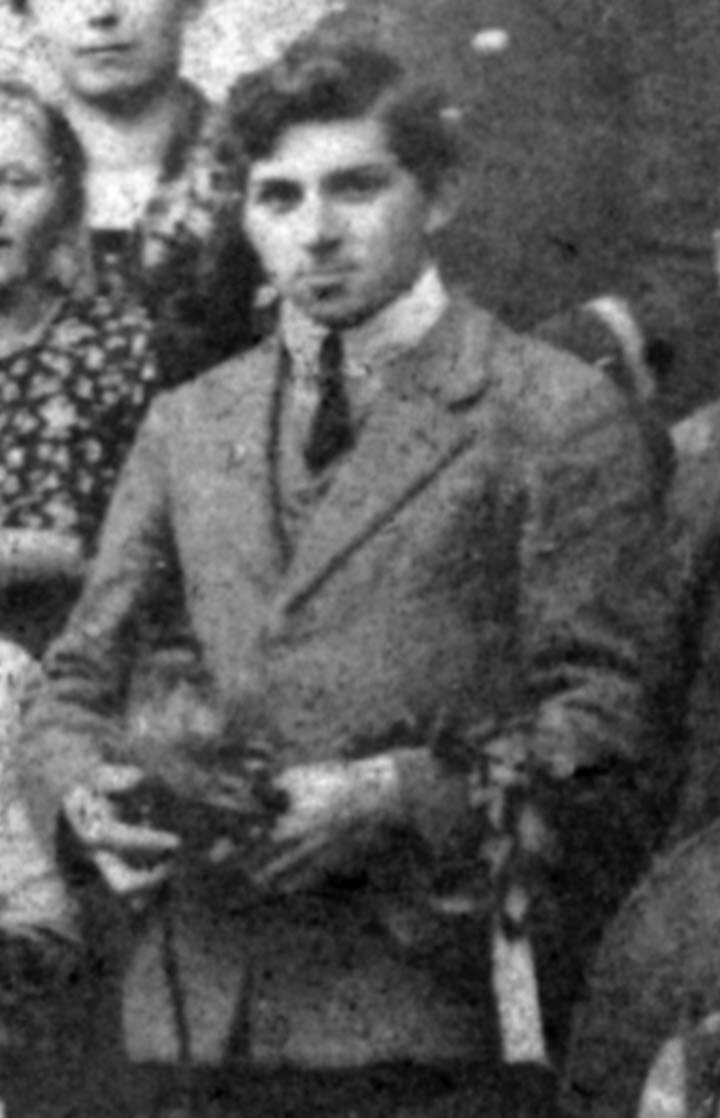
\includegraphics[width=4.209cm,height=6.507cm]{pictures/zulassungsarbeit-img027.jpg}

Max Rauscher\\
\end{supertabular}
\end{center}
\end{minipage}
\end{center}
Als Rauscher durch seine Anschuldigung Högn in den Streit mit hineinzog
und dieser mit markigen Worten offen die Kündigung Rauschers verlangte,
wurde eines deutlich: Ihr Verhältnis zueinander war offenbar auch
vorher nicht gut gewesen. Gehörte Högn nicht auch zu den Nörglern, die
schon zu Beginn von Rauschers Dienstzeit wenig Vertrauen in ihn setzten
und Rauscher während seiner 2-jährigen Dienstzeit die Arbeit schwer
machten, bis er es schließlich mit einer utopischen Gehaltforderung
bewusst auf die Kündigung anlegte? Högn wäre mit Sicherheit gerne
weiterhin Chorregent geblieben, wenn man, abgesehen vom finanziellen
Aspekt, die Abwechslung in der Tätigkeit betrachtet, die der
Chorregentendienst bot, sowie die Tatsache, dass Högn diesen Dienst mit
Leib und Seele ausführte. Die Anstellung Rauschers lieferte
letztendlich den Grund dafür, dass Kirchen- und Schuldienst nicht mehr
von einer Person ausgeübt werden durfte.

Eine Eintragung von Högn in einer Dirigierpartitur aus dem Notenbestand
der Ruhmannsfeldener Kirche ist beredtes Zeugnis dieser Rivalität
zwischen Rauscher und Högn. Rauscher hatte einen vermeintlichen
Vorzeichenfehler in der Partitur einer Messe von Vinzenz Goller
korrigiert. In einem rechthaberischen Ton schrieb Högn, der von der
Richtigkeit des gedruckten Notentextes überzeugt war, später den
Kommentar \zitat{„Grober Fehler! Nein! Muss „des“ heißen!“
}(Abb. 26) dazu, anstatt das eingefügte Vorzeichen einfach
auszuradieren, als hätte er der Nachwelt seine Zweifel an Rauschers
Kompetenz durch die Eintragung in die Partitur, die eigentlich nur er
selbst verwendete, mitteilen wollen.

\begin{center}
\begin{minipage}{4.142cm}
\begin{flushleft}
\tablefirsthead{}
\tablehead{}
\tabletail{}
\tablelasttail{}
\begin{supertabular}{m{3.9420002cm}}

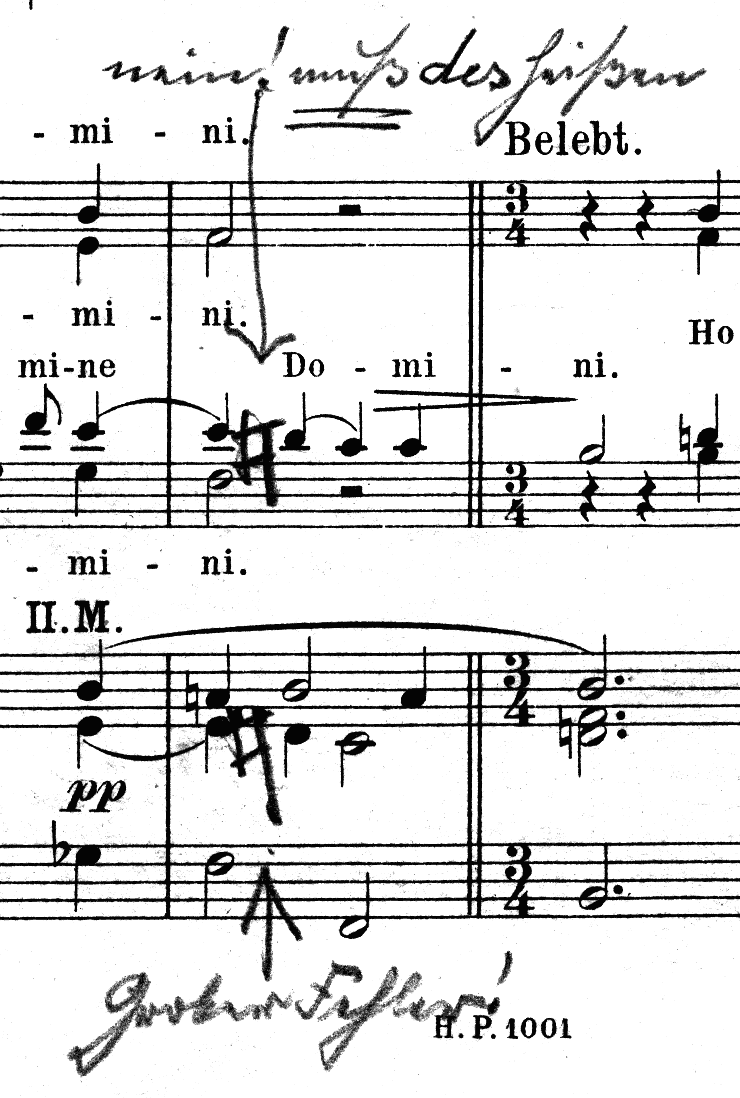
\includegraphics[width=3.759cm,height=5.547cm]{pictures/zulassungsarbeit-img028.png}

Eintragungen
von Max Rauscher und August Högn in eine Dirigierparitur\\
\end{supertabular}
\end{flushleft}
\end{minipage}
\end{center}
Pfarrer Fahrmeier schrieb nach der Kündigung Rauschers an die Regierung
von Niederbayern einen Brief, der den Zweck erfüllen sollte, eine
Ausnahmegenehmigung für die Übernahme des Chorregentendienstes durch
Högn zu erhalten. Dies zeigt, dass das Verhältnis Fahrmeier und Högn
anscheinend ein sehr gutes war. Nur Högn besitze, diesem Schreiben
zufolge die, \zitat{„zur Übernahme des Kirchenchores
notwendigen musikalischen Fähigkeiten und Kenntnisse“ }\footnote{
Dokument Nr. 12, Brief von der Kirchenverwaltung an die Regierung von
Niederbayern, 1.4.1927} und daher solle die zuständige Behörde den
Chorregentendienst von Högn \zitat{„bis auf weiteres“
} \footnote{Dokument Nr. 12, Brief von der Kirchenverwaltung an die
Regierung von Niederbayern, 1.4.1927} genehmigen. August Högn kannte
Fahrmeier schon lange vor seiner Ruhmannsfeldener Zeit. In Deggendorf
war Fahrmeier als Geistlicher zwischen 1896 und 1918 tätig.\footnote{
Reicheneder-Chronik, Seelsorger, Blatt III/13
(1) Vorderseite} Er konnte als Freund und Hauspfarrer der Familie Högn
in Deggendorf bezeichnet werden. Wenn er zur Ruhmannsfeldener Zeit
einen Ausflug nach Deggendorf unternahm, genehmigte er sich stets im
Hause Högn zuerst ein Bad, bevor er seinen Besorgungen in der Stadt
nachging. \footnote{Interview Nr. 3, Ida Högn, 29.12.2002, Absatz 10}

August Högns zweites Engagement in der Kirche von Ruhmannsfelden sollte
nur von begrenzter Dauer sein. Nur bis zu den Sommerferien 1927 sollte
die Regierung von Niederbayern Högns kirchenmusikalische Tätigkeit
genehmigen, \footnote{Dokument Nr. 13, Brief von der Kirchenverwaltung
an die Regierung von Niederbayern, 22.4.1927} bis ein pensionierter
Lehrer gefunden war, der die Chorregentenstelle längerfristig
übernehmen könnte. Doch unter der Ruhmannsfeldener Bevölkerung erhob
sich heftiger Widerstand gegen die Anstellung eines
Pensionisten, \footnote{Dokument Nr. 14, Brief von Alois Hartl an
Kirchenrat, 15.6.1927; Dokument Nr. 15, Brief von Johann Bielmeier an
Kirchenverwaltung, 17.6.1927} sodass die Stelle öffentlich
ausgeschrieben und von den fünf Kirchenmusiker, \footnote{Dokument Nr.
75, Bewerbung von Gottfried Hagemeiner, 25.10.1927} die sich beworben
hatten, entschied man sich für einen gewissen Georg Roßnagel. Sein
Dienstvertrag wurde zum Unterschreiben für den 7. Juni 1927 aufgesetzt.
Anscheinend hat Roßnagel seinen Dienst nie angetreten, denn derselbe
Dienstvertrag wurde zu einem späteren Zeitpunkt, mit ausgebesserten
Namen noch einmal bei der Anstellung von Albert Schroll verwendet, der
am 31. Juli 1929 diesen Vertrag mit der Kirche in Ruhmannsfelden
abschloss. Während der Name Schroll bei vielen Zeitzeugen bekannt war,
wusste nie etwas von einem Kirchenmusiker mit dem Namen Georg Roßnagel,
der laut Dienstvertrag zwei Jahre lang in Ruhmannsfelden gewirkt haben
soll. \footnote{Dokument Nr. 8, Dienstvertrag für Albert Schroll (Georg
Roßnagel), 31.7.1929 (7.6.1927)} Im Sommer 1929 trat Albert Schroll den
Chorregentendienst in Ruhmannsfelden an. Die auf wenige Wochen
beschränkte Aushilfe durch August Högn hat man am Ende auf über zwei
Jahre verlängert.

\begin{center}
\begin{minipage}{9.638cm}
\begin{center}
\tablefirsthead{}
\tablehead{}
\tabletail{}
\tablelasttail{}
\begin{supertabular}{m{4.333cm}m{4.905cm}}

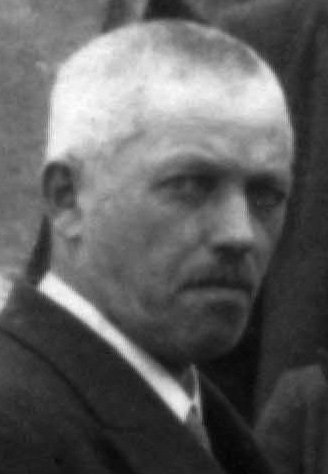
\includegraphics[width=4.15cm,height=6.006cm]{pictures/August-Hoegn_Nachruf.jpg}

August Högn &

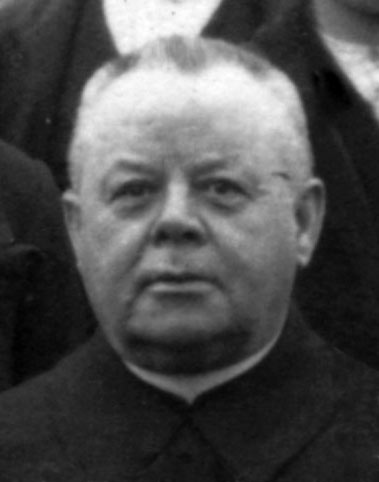
\includegraphics[width=4.722cm,height=5.994cm]{pictures/zulassungsarbeit-img029.jpg}

Karl Fahrmeier, in Ruhmannsfelden
Pfarrer von 1918 – 1935\\
\end{supertabular}
\end{center}
\end{minipage}
\end{center}

\subsection{Der Lehrer und Schulleiter}

1929 wurde August Högn zum
Oberlehrer ernannt. Dieser höhere Dienstgrad hatte ebenso wie seine
Ernennung zum Rektor 1940 bezüglich seines Aufgabenfeldes in der Schule
keinen Einfluss, da er schon seit 1921 Schulleiter war. Es war sicher
zur damaligen Zeit keine leichte Aufgabe, die Landschule zu leiten. Zum
einem war die finanzielle Lage der beteiligen Gemeinden, der so
genannten Schulsprengelverwaltung ziemlich angespannt, die für die
Instandsetzung der Schulgebäude einschließlich der Lehrerwohnungen und
die Beschaffung von Lehrmittel zuständig war. \footnote{Dokument Nr.
146, Brief von August Högn an Bürgermeister Forster, Ruhmannsfelden,
18.5.1936}

Zu manchen Zeiten wurden nicht einmal die notwendigen Lehrmittel im
erforderlichen Maße bereitgestellt. \footnote{Dokument Nr. 146, Brief
von August Högn an Bürgermeister Forster, Ruhmannsfelden, 18.5.1936}
Die finanziellen Engpässe wirkten sich natürlich ebenso auf den Zustand
der Schulgebäude aus. So konnten beispielsweise im Jahr 1934 die
Toiletten im so genannten Mädchenschulhaus eine Zeit lang gar nicht
mehr benutzt werden, da sie derart baufällig waren, dass laut Högn ihre
Benutzung lebensgefährlich für die Kinder war. \footnote{Dokument Nr.
144, Brief von August Högn an verstärkten Gemeinderat Ruhmannsfelden,
13.9.1934} Zum anderem schlug sich die schwierige Erwerbslage vieler
Familien negativ auf das Lernklima nieder. Besonders zur Erntezeit
mussten viele Kinder in der Landwirtschaft ihrer Eltern mithelfen, da
sich kaum eine Familie eine zusätzliche Arbeitskraft leisten konnte.
Aus diesem Grund war es zeitweise üblich, dass in den Sommermonaten der
Unterricht gekürzt werden musste. \footnote{Interview Nr. 6, Wilhelm
Ederer, 2.1.2003, Absatz 30} Eine dauerhafte Belastung für den
Schulbetrieb waren die langen Schulwege, die die Schüler aus am Rande
des großen Schulsprengels gelegenen Ortschaften und Höfen zu Fuß
zurücklegen mussten. Über eine Stunde dauernde Märsche zur Schule waren
keine Seltenheit und wurden bei Regen oder Schnee für die Schüler zur
Tortur. \footnote{Interview Nr. 6, Wilhelm Ederer, 2.1.2003, Absatz 10}

\begin{center}
\begin{minipage}{10.931cm}
\begin{flushleft}
\tablefirsthead{}
\tablehead{}
\tabletail{}
\tablelasttail{}
\begin{supertabular}{m{10.731cm}}

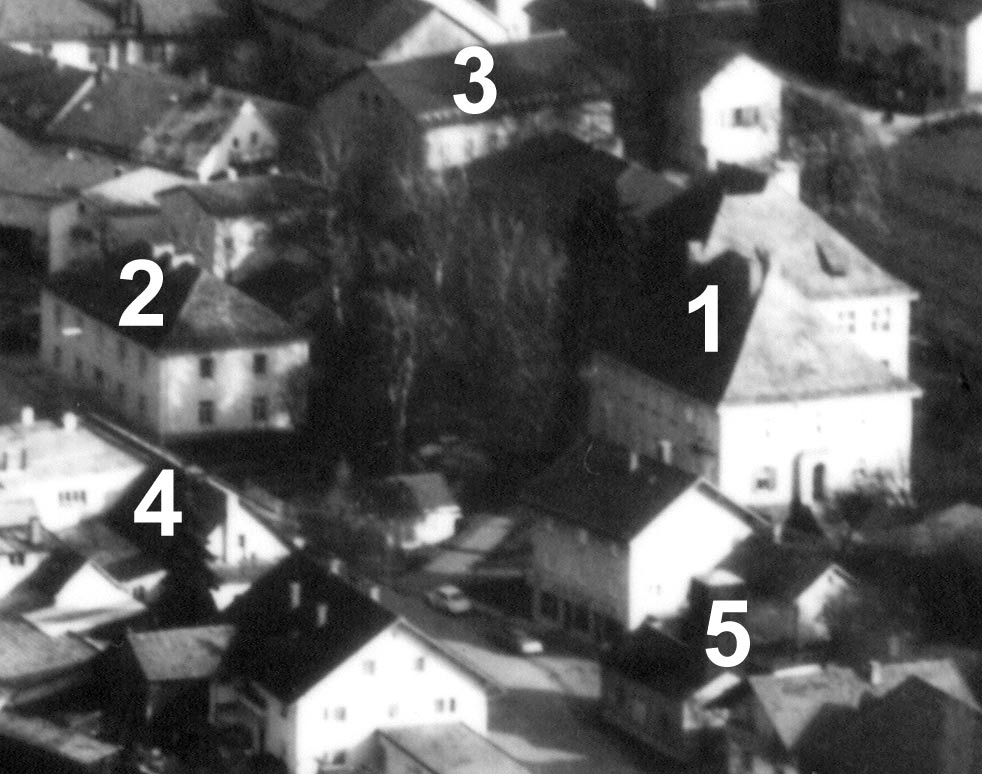
\includegraphics[width=10.548cm,height=8.313cm]{pictures/zulassungsarbeit-img030.jpg}

Schul- und Wohnhäuser von Högn:
\textbf{1:} Schulhaus von 1908: Hier wohnte August Högn 1932 – 1945,
\textbf{2:} Knabenschulhaus von 1834: Wohnung 1910 – 1932, \textbf{3:}
Mädchenschulhaus von 1884, \textbf{4:} Härtl-Haus: Wohnung 1945 – 1961,
\textbf{5:} Feuerwehrhaus\\
\end{supertabular}
\end{flushleft}
\end{minipage}
\end{center}
Wahrscheinlich lag es an den damals geringeren Anforderungen, die man an
eine Landschule stellte – überspitzt formuliert, war man schon froh,
wenn die Schüler regelmäßig am Unterricht teilnahmen – und an der
Positionen Högns als Schulleiter, dass er sich gewisse Dinge erlauben
konnte, die nicht regelkonform waren und in der heutigen Zeit undenkbar
wären. So ließ er beispielsweise die Schüler nicht nur für schulische
Zwecke, sondern auch für seine Privatangelegenheiten kleine Dienste und
Arbeiten während der Unterrichtszeit erledigen. Zu diesen Arbeiten
gehörten unter anderem einen Zettel von Klassenzimmer zu Klassenzimmer
tragen, \footnote{Interview Nr. 4, Maria Schröck, 30.12.2002, Absatz
46} Lehrmittel aus dem entsprechenden Zimmer holen, \footnote{Interview
Nr. 14, Johann Freisinger, 29.12.2003, Absatz 26} den Schulhof
aufräumen, das Pflaster am der Schule nahe gelegenen Kriegerdenkmal
ausgrasen \footnote{Interview Nr. 4, Maria Schröck, 30.12.2002, Absatz
14} und Holzaufrichten. \footnote{Korrespondenz Nr. 26, Brief von Franz
Danziger an Josef Friedrich, 25.2.2003; Interview Nr. 17, Max Holler,
26.8.2004, Absatz 16} Dies waren Dienste, die mit der Schule einen
gewissen Zusammenhang hatten, aber die Teppiche aus Högns Wohnung
klopfen, \footnote{Interview Nr. 6, Wilhelm Ederer, 2.1.2003, Absatz
34} von Högn geschossenes Wildfleisch zum Bahnhof bringen,\footnote{
Interview Nr. 17, Max Holler, 26.8.2004, Absatz 8} sein Rad
putzen \footnote{Interview Nr. 14, Johann Freisinger, 29.12.2003,
Absatz 24} oder sogar es reparieren \footnote{Interview Nr. 17, Max
Holler, 26.8.2004, Absatz 8} waren Arbeiten, die rein ins Private
fielen und jeden Bezug zur Schule entbehrten. Diese Tätigkeiten wurden
aber nicht als Strafarbeit, sondern als Zeichen besonderen Vertrauens
verstanden. \footnote{Korrespondenz Nr. 26, Brief von Franz Danziger an
Josef Friedrich, 25.2.2003}

{\centering
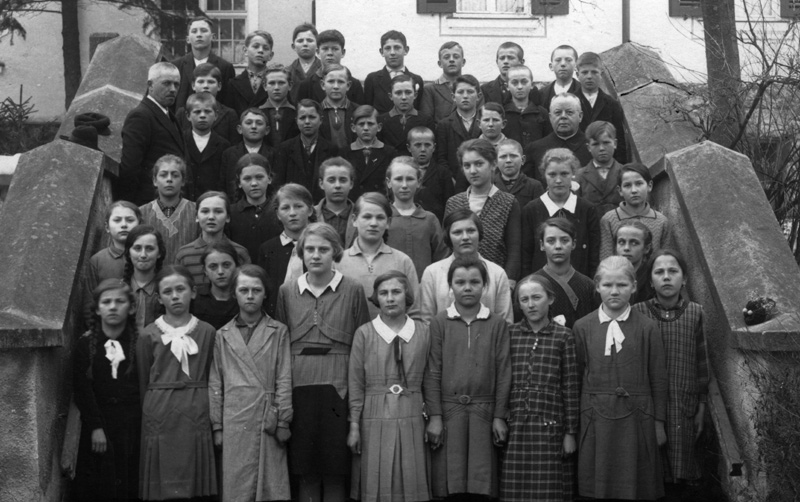
\includegraphics[width=16.044cm,height=10.081cm]{pictures/zulassungsarbeit-img031.jpg}
 \par}
Klassenfoto von 1932 mit August Högn
(links) und Pfarrer Fahrmeier (rechts)

Seitdem 1920 der Kirchendienst der Lehrer abgeschafft wurde, war der
Einsatz Högns als Organist bei Beerdigungen während der Unterrichtszeit
ein eindeutiger Verstoß gegen das damalige Schulrecht. Dass diese
Praxis auch noch zur NS-Zeit von den Behörden und der Seite der Eltern
toleriert wurde, lag an der besonders großen Macht der Institution
Kirche am Land. Eine gewöhnliche Beerdigung dauerte von 9 bis 11 Uhr,
so genannte „levitierte“ Beerdigungen für wohlhabende Verstorben
dauerten wesentlich länger. \footnote{Interview Nr. 4, Maria Schröck,
30.12.2002, Absatz 10} Högns Schüler mussten während seiner Abwesenheit
in Stillarbeit Aufgaben erledigen, ein paar Schüler wurden zu
Aufpassern ernannt \footnote{Interview Nr. 6, Wilhelm Ederer, 2.1.2003,
Absatz 8, Interview Nr. 4, Maria Schröck, 30.12.2002, Absatz 12;} und
die Lehrer der benachbarten Klassen statteten der „verwaisten Klasse“
hin und wieder einen Besuch ab. \footnote{Interview Nr. 4, Maria
Schröck, 30.12.2002, Absatz 10} Natürlich verhielten sich die Schüler
nicht nach Högns Vorstellung. Tumult im Klassenzimmer war noch das
kleinere Übel. Manchmal kam es sogar vor, dass sich einige Schüler
bereits auf den Nachhauseweg gemacht hatten, ehe Högn von der Kirche
ins Klassenzimmer zurückkehrte. Högn soll bei derartigen Vorkommnissen
des Öfteren versucht haben, diese Schüler mit dem Fahrrad einzuholen
und sie so zur Schule zurückzubringen. \footnote{Interview Nr. 6,
Wilhelm Ederer, 2.1.2003, Absatz 8}

\begin{center}
\begin{minipage}{6.202cm}
\begin{center}
\tablefirsthead{}
\tablehead{}
\tabletail{}
\tablelasttail{}
\begin{supertabular}{m{6.0020003cm}}

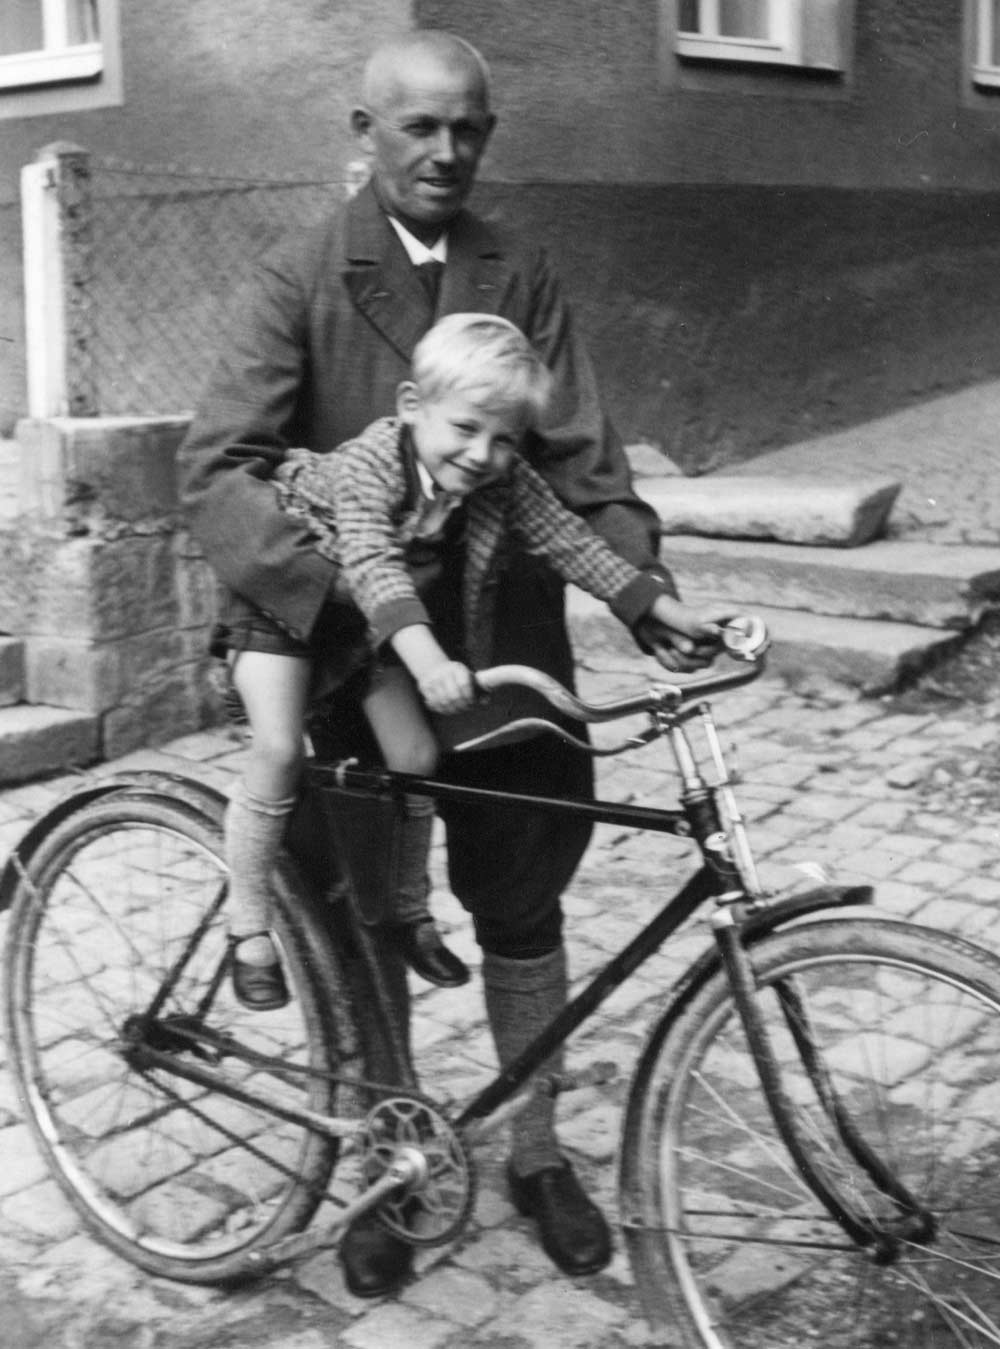
\includegraphics[width=5.821cm,height=7.851cm]{pictures/zulassungsarbeit-img032.jpg}

August Högn mit Enkel Werner
Schlumprecht und seinem Fahrrad 1939\\
\end{supertabular}
\end{center}
\end{minipage}
\end{center}
Die alltäglichen Beschwerlichkeiten, mit denen der damalige Lehrerstand
über all in Bayern zu kämpfen hatte – man bedenke die große
Schüleranzahl in einer Klasse – und die besonderen Schwierigkeiten in
Ruhmannsfelden schienen sich unter anderem auch in der Art
niedergeschlagen zu haben, wie Högn in der Klasse für Disziplin sorgte.
Viele der befragten Zeitzeugen bezeichneten August Högn als strengen
Lehrer. \footnote{Interview Nr. 3, Ida Högn,
29.12.2002, Absatz 6; Interview Nr. 14, Johann Freisinger, 29.12.2003,
Absatz 2; Interview Nr. 17, Max Holler, 26.8.2004, Absatz 16; Interview
Nr. 5, Barbara Essigmann, 2.1.2003, Absatz 18; Interview Nr. 24, Johann
Glasschröder, 28.12.2004, Absatz 12, 28} Dass er unfolgsame Schüler
mit Ohrfeigen, Tatzen \footnote{Interview Nr. 17, Max Holler,
26.8.2004, Absatz 12}, Ziehen an den Haarspitzen \footnote{Interview
Nr. 5, Barbara Essigmann, 2.1.2003, Absatz 20} und Schlägen auf den
Hintern \footnote{Interview Nr. 5, Barbara Essigmann, 2.1.2003, Absatz
18} bestrafte, ist daher kaum verwunderlich und außerdem üblich für die
damalige Zeit. Noch gewalttätigere Maßnahmen sind von ehemaligen
Schülern als Zeichen einer gewissen Hilflosigkeit verstanden worden,
die sie beim alternden und überforderten Lehrer beobachten konnten.
Hierzu gehörten Strafen, wie zum Beispiel Schülern die Schiefertafel so
stark über den zu Kopf schlagen, dass sie zerbrach, \footnote{Interview
Nr. 3, Ida Högn, 29.12.2002, Absatz 6} einen Bund mit vielen Schlüsseln
über den Kopf schlagen, \footnote{Interview Nr. 14, Johann Freisinger,
29.12.2003, Absatz 6} den Kopf der Schüler an die Tafel
stoßen, \footnote{Interview Nr. 14, Johann Freisinger, 29.12.2003,
Absatz 26; Interview Nr. 6, Wilhelm Ederer, 2.1.2003, Absatz 16} oder
sogar mit einem Blumentopf nach einem Schüler werfen.\footnote{
Interview Nr. 14, Johann Freisinger, 29.12.2003, Absatz 28} Ebenso gut
passen ungewöhnlich scharfe Beschimpfungen der Schüler mit Ausdrücken
wie etwa „ordinärer Hund“, \footnote{Interview Nr. 6, Wilhelm Ederer,
2.1.2003, Absatz 16} „dreckiger Hundschuft“ \footnote{Interview Nr. 17,
Max Holler, 26.8.2004, Absatz 16} oder „blöder Hammel“ \footnote{
Interview Nr. 5, Barbara Essigmann, 2.1.2003, Absatz 20} zum Bild des
alternden und überforderten Lehrers. Doch nicht nur mit harten Strafen,
die sich fester ins Gedächtnis ehemaliger Schüler eingruben, als
mancher pädagogische Kniff, versuchte er für Ruhe im Klassenzimmer zu
sorgen. Als geschickter Lehrer zeigte er sich, wenn er die Schüler am
Ende jeder Unterrichtsstunde zur Entspannung und Auflockerung aufstehen
ließ, um ihre überschüssigen Energien vor und nicht während der Stunde
loszuwerden. \footnote{Korrespondenz Nr. 26, Brief von Franz Danziger
an Josef Friedrich, 25.2.2003} Das negative Bild vom strafenden Lehrer
hebt sich auf, wenn Zeitzeugen ihren ehemaligen Lehrer trotz aller
seiner Wutausbrüche als sehr gerechten Lehrer bezeichnen.\footnote{
Interview Nr. 24, Johann Glasschröder, 28.12.2004, Absatz 12}

Als Entschädigung für manche Schwierigkeit im Schulalltag galt für den
leidenschaftlichen Musiker sicher der Musikunterricht. Dieser hatte den
größten Stellenwert unter allen Fächern, die Högn
unterrichtete. \footnote{Interview Nr. 17, Max Holler, 26.8.2004,
Absatz 10; Interview Nr. 4, Maria Schröck, 30.12.2002, Absatz 10;
Korrespondenz Nr. 26, Brief von Franz Danziger an Josef Friedrich,
25.2.2003} Zu manchen Zeiten wurde jeden Tag eine Stunde
gesungen. \footnote{Interview Nr. 5, Barbara Essigmann, 2.1.2003,
Absatz 20} Selbst als kurz vor Ende des 2. Weltkriegs ein Lehrer zwei
Klassen unterrichten musste – eine Klasse hatte täglich nur drei
Stunden Unterricht – wurde jeden Tag vor Beginn des Unterrichts statt
des Gebets ein Lied gesungen. \footnote{Interview Nr. 16, Maria
Freisinger, 25.8.2004, Absatz 22} Da die Volksschule Ruhmannsfelden
kein Klavier besaß, begleitete Högn die Volkslieder normalerweise auf
der Violine. \footnote{Interview Nr. 4, Maria Schröck, 30.12.2002,
Absatz 8; Interview Nr. 5, Barbara Essigmann, 2.1.2003, Absatz 20} Es
kam aber auch vor, dass die Lieder unbegleitet gesungen
wurden. \footnote{Interview Nr. 16, Maria Freisinger, 25.8.2004, Absatz
26} Nach Aussagen mehrerer ehemaliger Schüler sang man unter August
Högn durchaus mehrstimmig. \footnote{Interview Nr. 5, Barbara
Essigmann, 2.1.2003, Absatz 42; Interview Nr. 17, Max Holler,
26.8.2004, Absatz 42} Ein anfangs dreistimmiges, zum Schluss hin sogar
teilweise fünfstimmiges Arrangement Högns von dem Lied „Tauet Himmel“,
das mit „aus meinen Kinderliedern“ überschrieben ist, bestätigt dies.
Eine ehemalige Schülerin kann sich sogar an den Fall erinnern, als Högn
speziell für ihre Banknachbarin eine zweite Stimme arrangierte: Die
Schülerin sang einmal spontan zu einem einstimmigen Volkslied eine
zweite Stimme. Schon am nächsten Schultag legte ihr Högn eine
ausgeschriebene zweite Stimme vor. \footnote{Interview Nr. 16, Maria
Freisinger, 25.8.2004, Absatz 24} Beim Singen legte August Högn
durchaus Wert auf Stimmbildung. Er verlangte zum Beispiel, dass mit
Bruststimme \footnote{Interview Nr. 4, Maria Schröck, 30.12.2002,
Absatz 8} und im Stehen gesungen wurde, da sich so die
\zitat{„Lungen besser weite“} \footnote{Interview Nr. 5, Barbara Essigmann, 2.1.2003, Absatz
42}\zitat{ }könnten. Den Schülern standen Liederbücher zur
Verfügung, aus denen sie sich durchaus selbst Lieder zum Singen
aussuchen durften. \footnote{Interview Nr. 16, Maria Freisinger,
25.8.2004, Absatz 22} Es handelte sich wahrscheinlich um ein damals
gängiges Repertoire an allgemein bekannten Volksliedern, das gemeinsam
musiziert wurde. \footnote{Interview Nr. 5, Barbara Essigmann,
2.1.2003, Absatz 20} Aber auch politische Lieder wurden gesungen. Eine
Zeitzeugin berichtete, dass um 1930, also zur Zeit der
Rheinlandbefreiung und dem Aufkommen der deutsch-nationalen Bewegung,
häufiger patriotische Lieder wie z. B. das Lied „Kräftiger Zweig der
deutschen Eiche“ gesungen wurden. \footnote{Interview Nr. 4, Maria
Schröck, 30.12.2002, Absatz 6} Ab 28.12.1938 war der „Singkamerad“
 \footnote{Seite 129} das einzige an den bayerischen Volksschulen
zugelassene Liederbuch und von diesem Zeitpunkt an konnte man Lieder
vor allem mit NS-Gedankengut aus den Klassenzimmern hören. Högns
Klassen bildeten hier keine Ausnahme. \footnote{Interview Nr. 17, Max
Holler, 26.8.2004, Absatz 12}

\begin{center}
\begin{minipage}{8.807cm}
\begin{flushleft}
\tablefirsthead{}
\tablehead{}
\tabletail{}
\tablelasttail{}
\begin{supertabular}{m{8.607cm}}

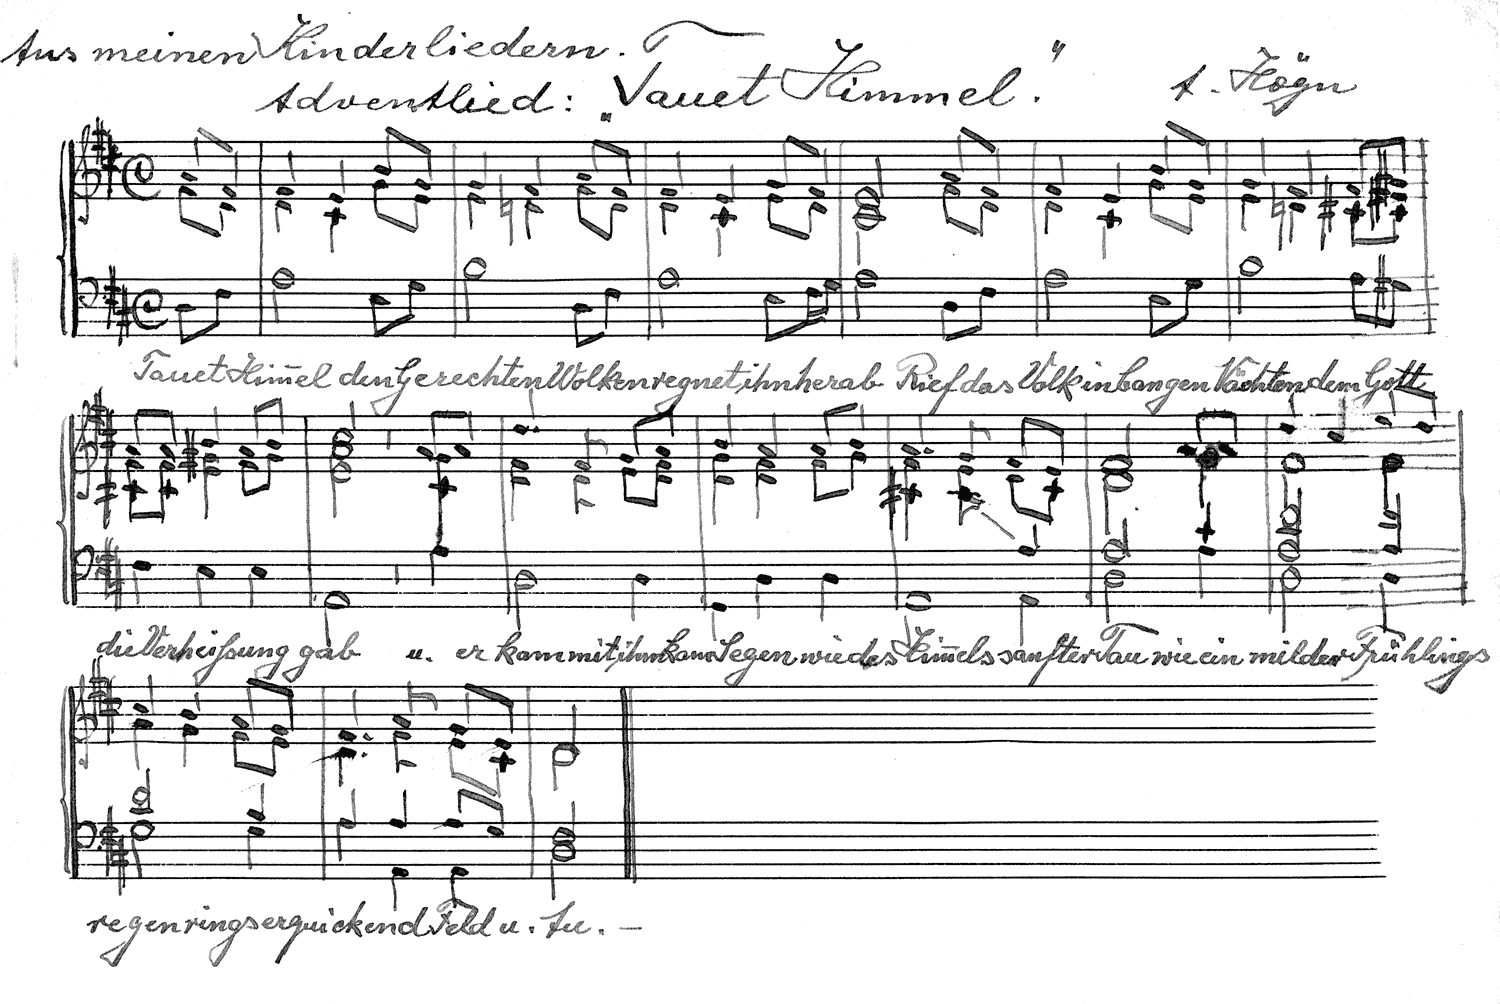
\includegraphics[width=8.373cm,height=5.604cm]{pictures/zulassungsarbeit-img033.png}

Arrangement des Liedes „Tauet Himmel“
von August Högn für den Schuleinsatz\\
\end{supertabular}
\end{flushleft}
\end{minipage}
\end{center}

\subsection{Högn und der Nationalsozialismus}

Aus
den Jahren 1936 und 1937 sind Dokumente erhalten, in denen August Högn
in der Funktion des Beauftragten für {\textquotedbl}Schutz des
Volksguts{\textquotedbl}, \footnote{Dokument Nr. 162, Brief von Albert
Schroll, Gemeindesekretär an August Högn, 21.1.1937}
Untergruppenführers \footnote{Dokument Nr. 128, Einteilung der
Gemeindegruppe Viechtach, 5.7.1937} und
Gemeindegruppenführers \footnote{Dokument Nr. 130, Brief von
Gemeindegruppenführer August Högn an alle Block- u. Hauswarte,
23.10.1936} hervortritt. Mit „Schutz des Volksguts“ wurden zur NS-Zeit
Metallsammlungen bezeichnet, an die sich auch die Schulen
beteiligten. \footnote{Interview Nr. 17, Max Holler, 26.8.2004, Absatz
16} Aus einem Dokument geht hervor, dass Högn als Führer der
Untergruppe Ruhmannsfelden der Gemeindegruppe Viechtach vier Blockwarte
unter sich hatte. \footnote{Dokument Nr. 128, Einteilung der
Gemeindegruppe Viechtach, 5.7.1937} In einem anderen Dokument
unterzeichnete der Gemeindegruppenführer Högn, wohl synonym gebraucht
zu Untergruppenführer, eine Einladung an alle Haus- und Blockwarte zur
Schulung im Luftschutz. Aufgrund der unvorstellbaren Verbrechen des
NS-Regimes sind Fragen nach der Zusammenarbeit des Einzelnen mit dem
damaligen Regime natürlich auch 60 Jahre nach Ende des 2. Weltkrieges
zu Recht von großer Brisanz. Doch sei vor voreiliger Vorverurteilungen
gewarnt, denn die wenigsten heute in der demokratischen Bundesrepublik
Deutschland lebenden Menschen haben diese totalitäre Diktatur mit ihren
indoktrinären Mechanismen bewusst miterlebt. Auch anhand einer noch so
drückend erscheinenden Beweislast, kann man letztlich doch nicht in
jemanden „hineinschauen“ und feststellen, ob stark das Engagement des
Einzelnen für den NS-Staat tatsächlich aus innerster Überzeugung
erfolgte. Anhand der im Folgenden geschilderten Fakten soll sich
deshalb jeder für sich selbst ein Bild von August Högn Einstellungs zur
Politik im 3. Reich machen.

Die Bewunderung, die Högn für seinen Schwiegersohn Dr. Karl
Schlumprecht, besonders für dessen politische Karriere zeigte\footnote{
Interview Nr. 20, Gertraud von Molo, 23.11.2004, Absatz 34} und das
gute Verhältnis zu ihm, \footnote{Interview Nr. 2, Barbara Essigmann,
27.12.2002, Absatz 66} sind Indizien dafür, dass Högn die Ideologie des
Nationalsozialismus nicht von Grund auf ablehnt hat. Dr. Karl
Schlumprecht war nach der Machtübernahme der NSDAP erster
nationalsozialistischer Oberbürgermeister von Bayreuth bis April
1937. \footnote{http://www.bnbt.de/\~{}tr1035/bt/wer/index.htm} Später
war er als Ministerialdirektor im Finanzministerium in München
tätig \footnote{Dokument Nr. 99, Brief von Bürgermeister Sturm an Dr.
Karl Schlumprecht, 1.9.1938} und stieg sogar zum Wirtschaftminister von
Bayern auf (16.7.1943 – 21.4.1944).\footnote{
http://www.stmwivt.bayern.de/das\_ministerium/geschichte\_staatsministerium.html}
Vor allem der berufliche Werdegang Schlumprechts war der Grund, weshalb
Högn auf seinen Schwiegersohn so stolz war. Er wäre es sicherlich nicht
gewesen, hätte er die NS-Ideologie in den Grundzügen ablehnt.

\begin{center}
\begin{minipage}{6.969cm}
\begin{flushleft}
\tablefirsthead{}
\tablehead{}
\tabletail{}
\tablelasttail{}
\begin{supertabular}{m{6.769cm}}

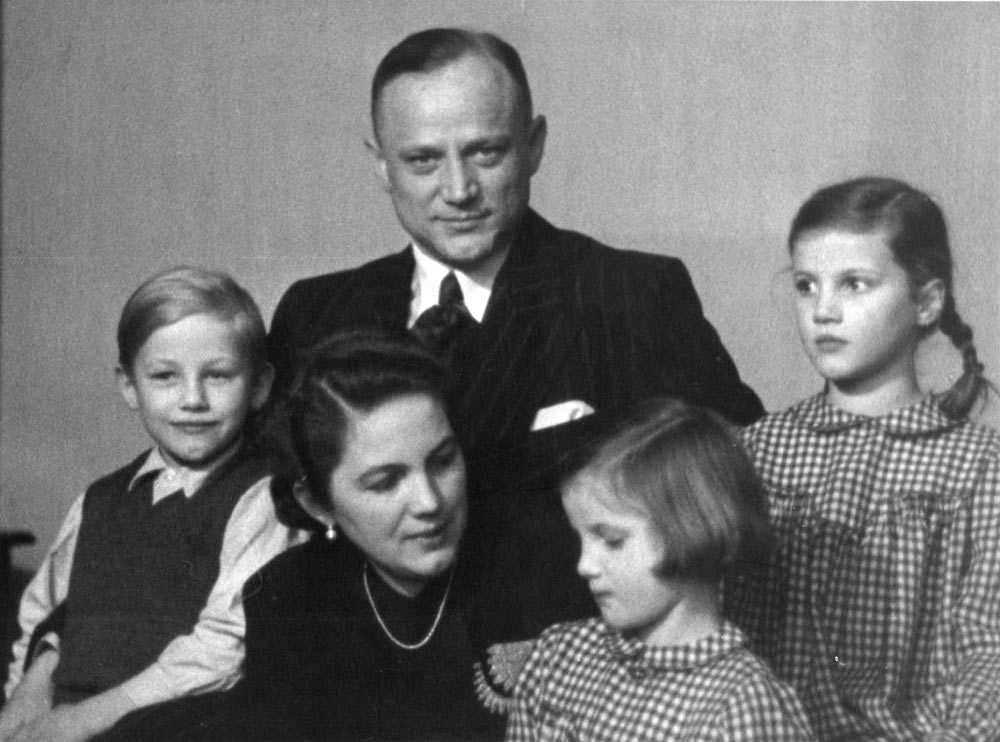
\includegraphics[width=6.588cm,height=4.888cm]{pictures/zulassungsarbeit-img034.jpg}

Dr. Karl Schlumprecht mit seiner Frau,
der Högn Tochter Frieda, und den Kindern Werner, Gertraud und Lilo\\
\end{supertabular}
\end{flushleft}
\end{minipage}
\end{center}
Högn wusste den guten Draht zu einem hohen NS-Funktionär zu nutzen –
nicht zum eigenen Vorteil, sondern zu dem der Allgemeinheit. Der
damalige Ruhmannsfeldener Bürgermeister Sturm stellte am 1. September
1938 an den Ministerialdirektor Schlumprecht im Finanzministerium einen
Antrag auf Unterstützung bei der Finanzierung des Außenputzes der
Ruhmannsfeldener Turnhalle. Der Vermerk auf dem Brief „In Abdruck an H.
Oberlehrer Högn, hier zur Kenntnis“ zeigt eindeutig, dass diese
Petition durch Högn, den ehemaligen Turnvereinsvorstand und
Veranstalter von Benefizkonzerten zugunsten der Errichtung der
Turnhalle, eingefädelt worden war. \footnote{Dokument Nr. 99, Brief von
Bürgermeister Sturm an Dr. Karl Schlumprecht, 1.9.1938}

Der Tatsache, dass Högn alle 12 Jahre des „1000-jährigen Reichs“
Schulleiter geblieben war, sagt zumindest aus, dass er den
Regimeführenden nicht negativ aufgefallen war. Seine Ernennung 1940 zum
Rektor der Volksschule zeigte, dass er zumindest auf der vorgegeben
Linie blieb. \footnote{Dokument Nr. 48, Zeitungsartikel aus Viechtacher
Bayerwald-Bote, 2.8.1958}

Eine Komposition mit eindeutig nationalsozialistischem Text lässt sicher
Rückschlüsse auf August Högns Gesinnung im 3. Reich zu. Auf den
Rückseiten der Notenblätter des Arrangements „Näher mein Gott zu dir!“
ist ein „Weihegesang“ zu finden. Auf jedem Notenblatt des Weihegesangs
steht „A. Högn“, wie bei allen August Högn eindeutig zugeordneten
Kompositionen. Högn hatte den Weihegesang nur durchgestrichen und das
Notenpapier weiter verwendet. Dieses Notenpapier war im Notenschrank
der Pfarrkirche St. Laurentius in Ruhmannsfelden aufzufinden. Hat
dieses der Komposition Högns zu Grunde liegende Gedicht – sein
Verfasser ist ungekannt – in der ersten Strophe noch Ähnlichkeit mit
Högns geistlicher Komposition, dem „Grablied für die auf dem Felde der
Ehre Gefallen op. 35“, so wird spätestens in der dritten Strophe klar,
wenn von „Steigt ein, der aus Walhallas Höhe, hoch ist es Zeit zur Tat“
die Rede ist und damit wohl die „Vorsehung“ Hitlers gemeint ist, dass
es sich nicht nur um einen patriotischen, sondern
nationalsozialistischen Text handelt. Der Weihegesang wurde mit
Sicherheit einige Male bei der weltlichen Trauerfeier für gefallene
Soldaten aufgeführt, die vor dem kirchlichem Requiem
stattfand, \footnote{Interview Nr. 6, Wilhelm Ederer, 2.1.2003, Absatz
6} da die mit Tinte geschriebenen Stimmen Flecken aufweisen, wie sie
nur Regentropfen verursachen können. Besonders irritiert, dass der
Weihegesang sowohl stilistisch als auch bezüglich der Besetzung, kaum
einen Unterschied zu den von Högn komponierten christlichen Grabliedern
ausmacht (siehe  „Weihegesang Es-Dur“, Seite
). Wie August Högn selbst zum Inhalt dieses
Texts stand, den er vertont hat, wird wohl unbekannt bleiben. Man kann
davon ausgehen, dass von der nationalsozialistischen Partei an ihn
Anfragen erfolgten, nicht nur die Gestaltung der geistlichen, sondern
auch der weltlichen Trauerfeier zu übernehmen. Wie er es in allen
anderen musikalischen Feldern gewohnt war, griff Högn auch hier zur
Feder, um passende Musik zu dem passenden Text zu schreiben. Doch
ernsthafte Konsequenzen wären sicher ausgeblieben, wenn er die Bitten
ausgeschlagen und schon gar nicht, wenn er ein Werk eines anderen
Komponisten aufgeführt hätte.

\begin{center}
\begin{minipage}{8.835cm}
\begin{center}
\tablefirsthead{}
\tablehead{}
\tabletail{}
\tablelasttail{}
\begin{supertabular}{m{8.635cm}}

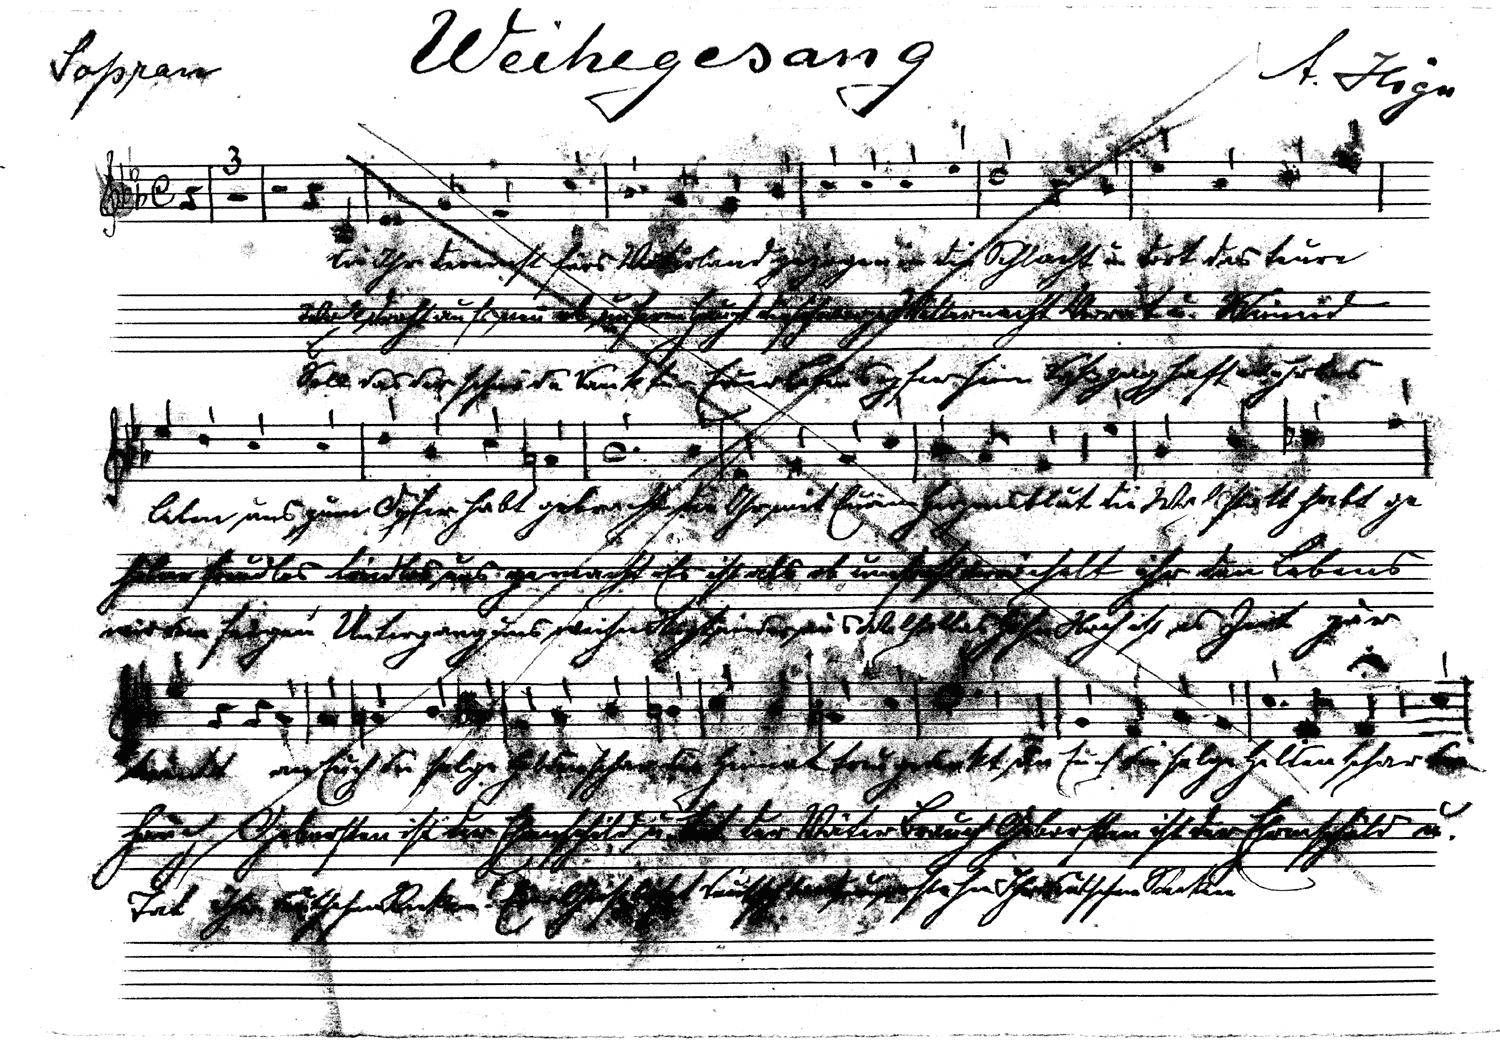
\includegraphics[width=8.453cm,height=5.678cm]{pictures/zulassungsarbeit-img035.png}

Sopran-Stimme des Weihegesang Es-Dur\\
\end{supertabular}
\end{center}
\end{minipage}
\end{center}
Als treuer Parteianhänger ist August Högn jedoch keinem der sechs zu
diesem Thema befragten Zeitzeugen in Erinnerung geblieben.\footnote{
Interview Nr. 4, Maria Schröck, 30.12.2002, Absatz 24; Interview Nr. 6,
Wilhelm Ederer, 2.1.2003, Absatz 24 – 26; Interview Nr. 16, Maria
Freisinger, 25.8.2004, Absatz 40; Interview Nr. 17, Max Holler,
26.8.2004, Absatz 18; Interview Nr. 24, Johann Glasschröder,
28.12.2004, Absatz 18; Interview Nr. 26, Eva Ertl, 9.2.2005, Absatz 28}
Als fanatische Anhängering der NS-Ideologie prägten sich einige der
Befragten stattdessen die seit 1942 \footnote{Reicheneder-Chronik,
Schulwesen, Blatt 112 Rückseite} an der Volksschule Ruhmannsfelden
unterrichtende Lehrerin Charlotte Werner ein. In ihrem Unterricht
musste Schüler aus einem Kalender Vorträge über herausragende
Persönlichkeiten des NS-Regimes halten. Vergleichbares ist aus Högns
Unterricht nicht bekannt. \footnote{Interview Nr. 6, Wilhelm Ederer,
2.1.2003, Absatz 24 – 28}

Rückschlüsse auf Högns Einstellung zu Hitlers Politik lassen sich nicht
zuletzt aus seinem in der Nachkriegszeit entstandenen Geschichtswerk
lesen. Folgende Textpassage aus der „Geschichte von Zachenberg“ lässt
sogar einen Interpretationsspielraum offen im Bezug auf seine anfangs
positive Einstellung zur NS-Ideologie, die sich im Lauf der Zeit hin
zur Ablehnung verändert haben könnte: \textit{„Die 1932/33
hereinbrechende Hitlerzeit hat zwar auf der einen Seite dieser
schlimmen Arbeitslosigkeit ein Ende gesetzt, aber auf der anderen Seite
den unheilvollen zweiten Weltkrieg heraufbeschworen, der das größte
Unglück, das je über ein Land und seine Bevölkerung kommen konnte, in
übervollem Maße über Deutschland ausgeschüttet hat.“ } \footnote{Högn,
Zachenberger, Blatt 17 (erster Teil)}\textit{ }Als ob er sich selbst
für seine anfängliche Gefolgschaft Hitlers rechtfertigen will, führt er
die Bekämpfung der Arbeitslosigkeit durch Hitler als eine zu würdigende
Errungenschaft an, geht aber sehr deutlich auf Distanz zur späteren
NS-Politik, die die „Kriegsfurie“, \footnote{Högn, Ruhmannsfelden,
Seite 16} – so nennt er den 2. Weltkrieg in der „Geschichte von
Ruhmannsfelden“ – verursacht hat, als er vollständig dessen Folgen
aufzählt. Wie ein Läuterungsversuch erscheinen die ausgedehnten
Passagen in seiner „Geschichte von Ruhmannsfelden,“ in denen er den
beiden Ruhmannsfeldener Widerständlern, Bürgermeister Sturm und
Studienrat Leonhard Donauer, die nur mit viel Glück der Exekution durch
die SS entronnen waren, ein Denkmal setzt. \footnote{Högn,
Ruhmannsfelden, Seite 32}

\begin{center}
\begin{minipage}{4.928cm}
\begin{flushleft}
\tablefirsthead{}
\tablehead{}
\tabletail{}
\tablelasttail{}
\begin{supertabular}{m{4.728cm}}

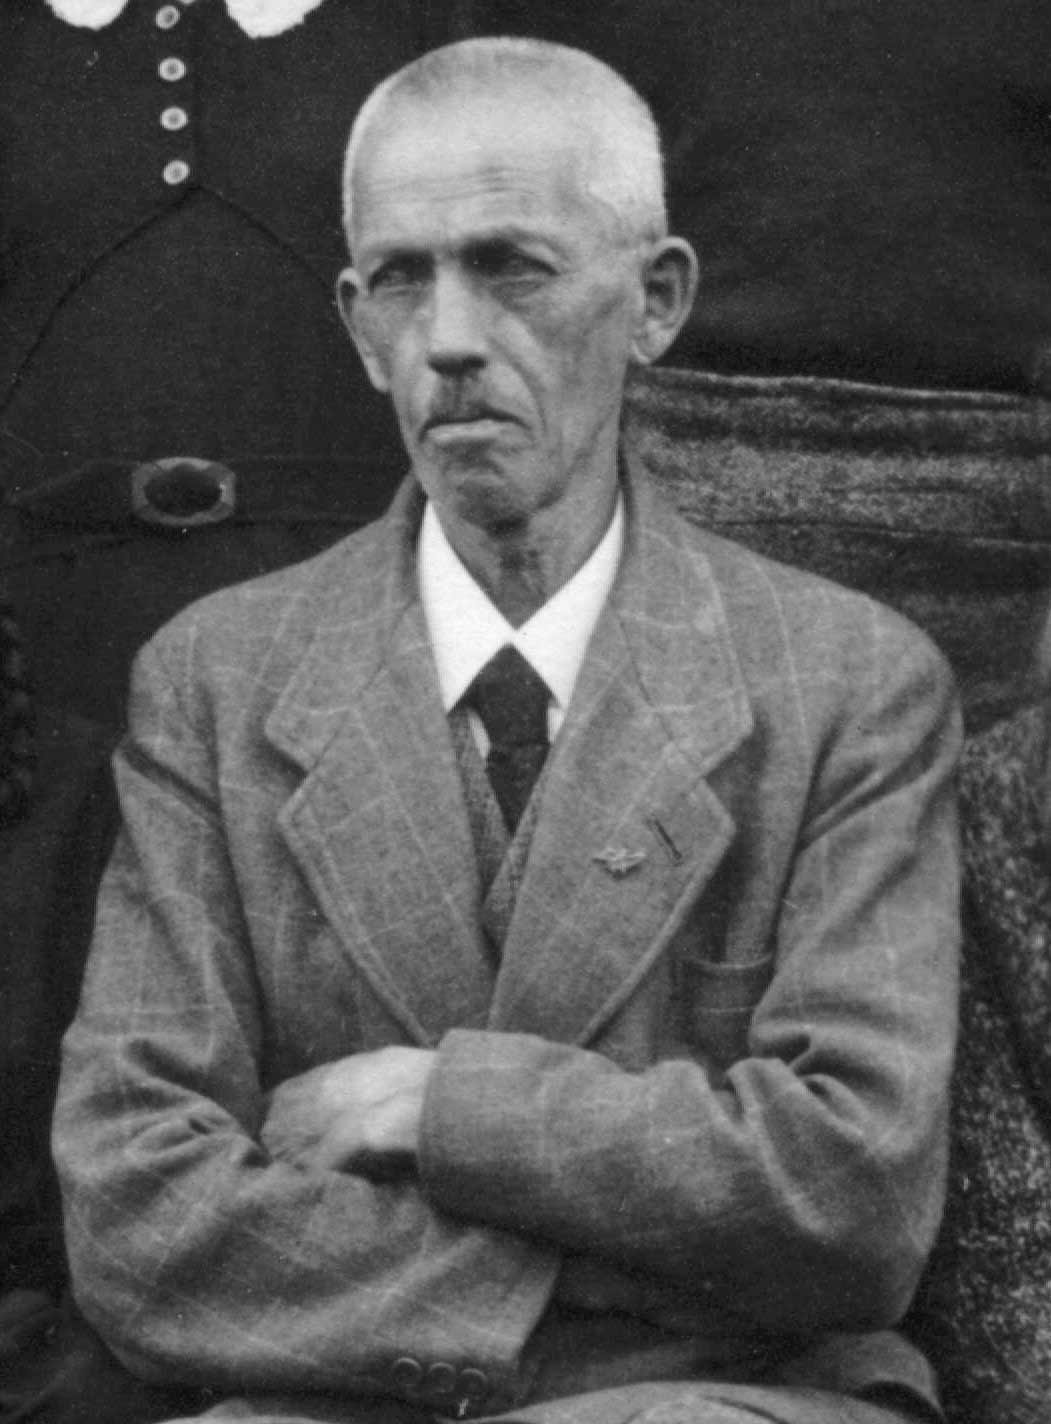
\includegraphics[width=4.503cm,height=6.103cm]{pictures/zulassungsarbeit-img036.jpg}

August Högn 1944: Das Bild eines eher
im inneren Konflikt lebenden, gebrochenen Mannes als das eines stolzen,
überzeugten Nazis.\\
\end{supertabular}
\end{flushleft}
\end{minipage}
\end{center}
Außer Frage steht, dass Högn kein Rassist war. Franz Danziger,
Kirchenchorsänger, Violinist und schließlich Högns Nachfolger als
Chorregent, war ein Halbjude, wie er im Jargon der Nationalsozialisten
geheißen hätte. Er erwähnte in seinen Memoiren über Högn kein einziges
schlechtes Wort. Viel mehr ehrte er seinen ehemaligen Lehrer, indem er
einige seiner Kompositionen aufführte.

Högns Chorregententätigkeit während des Krieges ist ebenfalls ein
Anhaltspunkt dafür, dass Högn nicht in allen Bereichen im Sinne der
NS-Ideologie gehandelt hat. Ein wirklich überzeugter Anhänger der
Weltanschauung Hitlers hätte versucht Religionen eher zu bekämpfen, als
sie durch Chorleiter- und Organistendienste doch maßgeblich zu fördern.

\subsection{Chorregent in schwieriger Zeit}
\hypertarget{RefHeadingToc100333735}{}Am 25.1.1940 starb der erst 36
Jahre alte Chorregent und Gemeindesekretär Albert Schroll, der 10 Jahre
lang in Ruhmannsfelden wirkte. \footnote{Korrespondenz Nr. 90, Brief
von Pfarramt Kollnburg an Josef Friedrich, 13.1.2005} Er erkrankte
schon 1939, sodass der Lehrer Ertl für Schroll als Klavierbegleiter bei
einem Singspiel einspringen musste. \footnote{Interview Nr. 16, Maria
Freisinger, 25.8.2004; Absatz 44} August Högn vertrat Schroll als
Chorregent und Organist während seiner Krankheit und nach dessen Tod
übernahm er seine Stelle \footnote{Interview Nr. 2, Barbara Essigmann,
27.12.2002, Absatz 6} aushilfsweise, wie es den Chorabrechnungen zu
entnehmen ist. \footnote{Dokument Nr. 136, Chorabrechnung Beerdigungen
und Trauungen, 3. Quartal 1952; Dokument Nr. 137, Chorabrechnung Ämter
und Messen, 3. Quartal 1952} Der 61-jährige und daher nicht mehr
wehrfähige Högn blieb aber Chorregent und Organist während des gesamten
2. Weltkriegs, da aufgrund der Kriegssituation kein hauptamtlicher
Kirchenmusiker als Nachfolger für Schroll verfügbar war. Nach dem Krieg
wurde Högn infolge der Entnazifizierung vom Schuldienst suspendiert und
dann in den Ruhestand versetzt, sodass der Weiterführung der
Chorregententätigkeit durch Högn in Form der Unvereinbarkeit von Schul-
und Kirchendienst nichts mehr im Wege stand. Zu Beginn von Högns
dritter Chorregentenzeit kehrte man gezwungenermaßen zur gewohnten
Praxis zurück, bei Beerdigungen den Unterricht ausfallen zu
lassen. \footnote{Interview Nr. 16, Maria Freisinger, 25.8.2004, Absatz
6; Interview Nr. 6, Wilhelm Ederer, 2.1.2003, Absatz 6} Diese in der
Weimarer Republik geduldete Regelung wurde von den Behörden des
religionsfeindlichen NS-Regimes bald unterbunden. Josef Brunner – er
war zu jung für den Kriegseinsatz \footnote{Interview Nr. 8, Josef
Brunner, 3.1.2003, Absatz 2} – und eine Mallersdorfer Schwester, die an
der Kinderbewahranstalt arbeitete, übernahmen deshalb den
Organistendienst bei Beerdigungen an Stelle von August Högn.\footnote{
Interview Nr. 16, Maria Freisinger, 25.8.2004, Absatz 6}

\begin{center}
\begin{minipage}{5.593cm}
\begin{flushleft}
\tablefirsthead{}
\tablehead{}
\tabletail{}
\tablelasttail{}
\begin{supertabular}{m{5.393cm}}

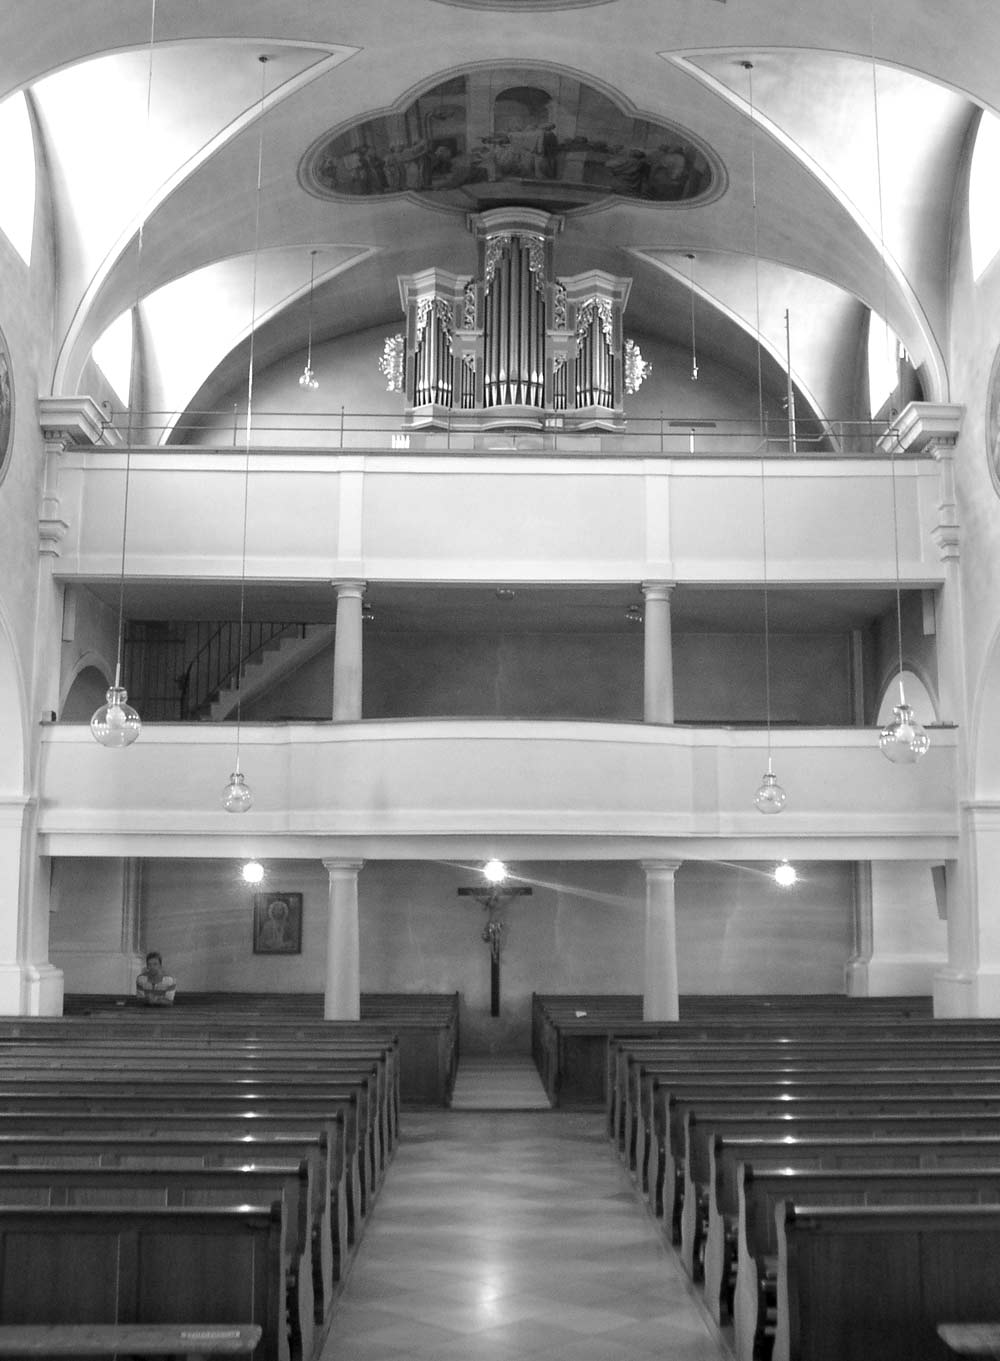
\includegraphics[width=5.001cm,height=6.805cm]{pictures/zulassungsarbeit-img037.jpg}

Pfarrkirche St. Laurentius
Ruhmannsfelden, Blick zur Orgelempore\\
\end{supertabular}
\end{flushleft}
\end{minipage}
\end{center}
Högns 3. Dienstzeit als Chorregent durchlief eine der schlimmsten Phasen
– nicht nur für die Kirchenmusik: Die Zeit des 2. Weltkriegs. Schon
1939 wurden vier Lehrer, die im Orchester mitwirkten,\footnote{
Interview Nr. 2, Barbara Essigmann, 27.12.2002, Absatz 4} zum
Kriegsdienst eingezogen. \footnote{Reicheneder-Chronik, Schulwesen,
Blatt 112 Vorder- und Rückseite} Einheimische Musiker des Orchesters,
wie Lorenz Schlagintweit, blieben von einem Kriegseinsatz genauso wenig
verschont. \footnote{Interview Nr. 13, Lorenz Schlagintweit,
29.11.2003, Absatz 2} Große Aufführungen mit Orchester an Festtagen,
wie von mehreren Zeitzeugen berichtet, \footnote{Interview Nr. 12,
Emilie Seidl, 23.4.2003, Absatz 14} dürften daher eher vor Ausbruch des
2. Weltkriegs, also zur Zeit von Chorregent Schroll, stattgefunden
haben. Besonders für das Streichorchester stellte der Krieg einen Bruch
dar. Als Ersatz etablierte sich eine Blechbläserformation, die sich aus
älteren Musikern der umliegenden Blaskapellen zusammensetzte. Die
Männerstimmen des Kirchenchores waren den Umständen entsprechend mit
nur zwei Sängern, nämlich Schwannberger und Holzfurtner, dünn
besetzt. \footnote{Interview Nr. 16, Maria Freisinger, 25.8.2004,
Absatz 6} Auch von der Orgel der Ruhmannsfeldener Pfarrkirche forderte
der Krieg seinen Tribut. Angesichts des geringen Metallgewinns, den die
am 12.6.1944 zum Ausbau bestimmten dünnwandigen Pfeifen und Leitungen
erbrachten, wird einerseits die aussichtslose Lage der
Kriegswirtschaft, andererseits die bewusste Schikane der Nazis
gegenüber der Kirche deutlich. Die Orgel – ihr fehlten die Register
Quintatön, Vox coelestis des ersten und alle metallischen Pfeifen
einschließlich der Windleitungen des zweiten Manuals\footnote{
Reicheneder-Chronik, Orgel, Blatt 74 Rückseite} – erlitt in der
Nachkriegszeit durch eine lange Trockenheit zusätzlichen großen
Schaden, ehe die Orgel 1947 vom Orgelbaumeister Kratochwill aus
Plattling restauriert wurde. \footnote{Högn, Ruhmannsfelden, S. 29}

Ob Högns Probenpraxis – die Proben fanden in seiner Wohnung
statt \footnote{Interview Nr. 2, Barbara Essigmann, 27.12.2002, Absatz
32} – eine Anpassung an den durch den Krieg geschmälerte Chor war oder
ob der Probenort auch schon in seiner ersten und zweiten
Chorregentenzeit derselbe war, kann aus Mangel an Zeitzeugen der
früheren Chorregentenzeiten nicht geklärt werden. Die Probenarbeit in
seiner Dienstwohnung hatte für Högn im allgemeinem einige praktische
Vorteile, und zwar aus folgenden Gründen: Hätte der Chor in der Kirche
geprobt, wäre es vor allem im Winter besonders kalt gewesen, da auf der
Orgelempore ein Fenster undicht war. \footnote{Interview Nr. 5, Barbara
Essigmann, 2.1.2003, Absatz 26} Einen beheizten Proberaum konnte die
Pfarrgemeinde damals nicht zu Verfügung stellen, sodass Högns große
Lehrerwohnung willkommene Alternative zur Kirche war. Außerdem besaß
Högn keinen Kirchenschlüssel, sodass er dem Mesner hätte Bescheid geben
müssen, damit die Kirche abends offen blieb. Nach der Probe hätte Högn
den Schlüssel im Pfarrhof zurückgeben müssen, was an sich relativ
umständlich gewesen wäre. \footnote{Interview Nr. 2, Barbara Essigmann,
27.12.2002, Absatz 88} Einige Zeitzeugen behaupten, dass nicht nur eine
einzige Stimmgruppe \footnote{Interview Nr. 2, Barbara Essigmann,
27.12.2002, Absatz 34} oder der komplette Chor in seiner Wohnung
probte, sondern auch das Blechbläserquartett. Nur die Generalprobe fand
in der Kirche statt. \footnote{Interview Nr. 13, Lorenz Schlagintweit,
29.11.2003, Absatz 4} Die Proben wurden auch nicht regelmäßig
abgehalten, beispielsweise jede Woche an einem bestimmten Wochentag,
sondern fanden nur dann statt, wenn ein neues Repertoire für große
Festtage erarbeitet werden musste. \footnote{Interview Nr. 2, Barbara
Essigmann, 27.12.2002, Absatz 48} Eine regelmäßige Probenarbeit machte
anscheinend wenig Sinn, wenn man sich den täglichen Einsatz der
Hauptsänger und –sängerinnen an den Gottesdiensten vergegenwärtig.
Durch die vielen Aufführungen hatte der Chor Routine und manche
Probearbeit wurde nach den Gottesdiensten geleistet.\footnote{
Interview Nr. 5, Barbara Essigmann, 2.1.2003, Absatz 36}

Vielleicht ist es aber auch auf die Proben in der privaten Wohnung
zurückzuführen, dass die Kirchenmusik in Ruhmannsfelden dem
deutschlandweiten Kulturaufschwung nach Ende des Krieges nicht folgte,
– man denke an die vielen Kleinkunstbühnen, die aus dem Boden schossen,
oder Konzerte, die in den Ruinen der ehemaligen Konzertsäle abgehalten
wurden – sondern eher einen Niedergang erlebte. \footnote{Interview Nr.
9, Dr. Doraliesa Wiegmann, 19.1.2003, Absatz 4; Interview Nr. 24,
Johann Glasschröder, 28.12.2004, Absatz 36} Die in Högns Wohnung
abgehaltenen Proben schienen zu einer Privatveranstaltung verkommen zu
sein. Nur für die Hauptsängerinnen hielt Högn Proben nach Ende des 2.
Weltkriegs. Die Sängerin Maria Freisinger hat jahrelang sonntags an den
Gottesdiensten mitgewirkt, doch an Proben konnte sie sich nicht
erinnern. \footnote{Interview Nr. 16, Maria Freisinger, 25.8.2004,
Absatz 8} Der öffentliche Chor wurde zu einem nach außen hin
abgeschlossenen Zirkel von eng befreundeten Hauptsängerinnen, zu dem
nur schwer neue Mitglieder stoßen konnten.

\begin{center}
\begin{minipage}{3.491cm}
\begin{flushleft}
\tablefirsthead{}
\tablehead{}
\tabletail{}
\tablelasttail{}
\begin{supertabular}{m{3.291cm}}

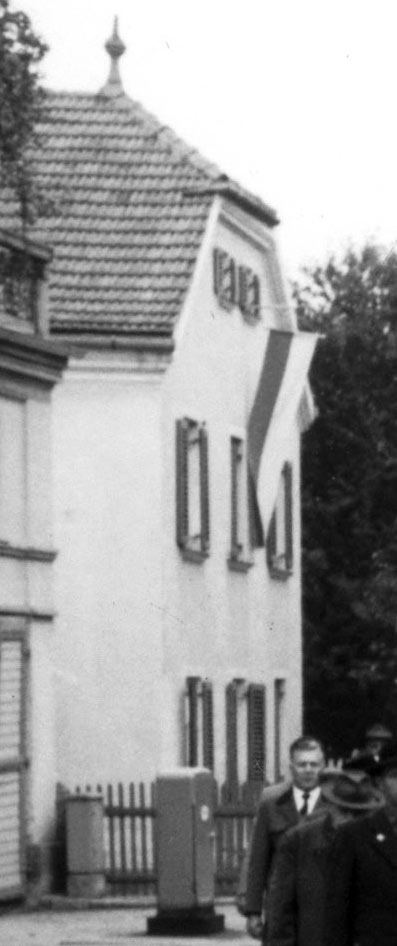
\includegraphics[width=3.108cm,height=7.408cm]{pictures/zulassungsarbeit-img038.jpg}

Im Erdgeschoss dieses Hauses wohnte
Högn ab 1945 bis zu seinem Tod\\
\end{supertabular}
\end{flushleft}
\end{minipage}
\end{center}
\begin{flushleft}
\tablefirsthead{}
\tablehead{}
\tabletail{}
\tablelasttail{}
\begin{supertabular}{m{4.6330004cm}}

\begin{center}

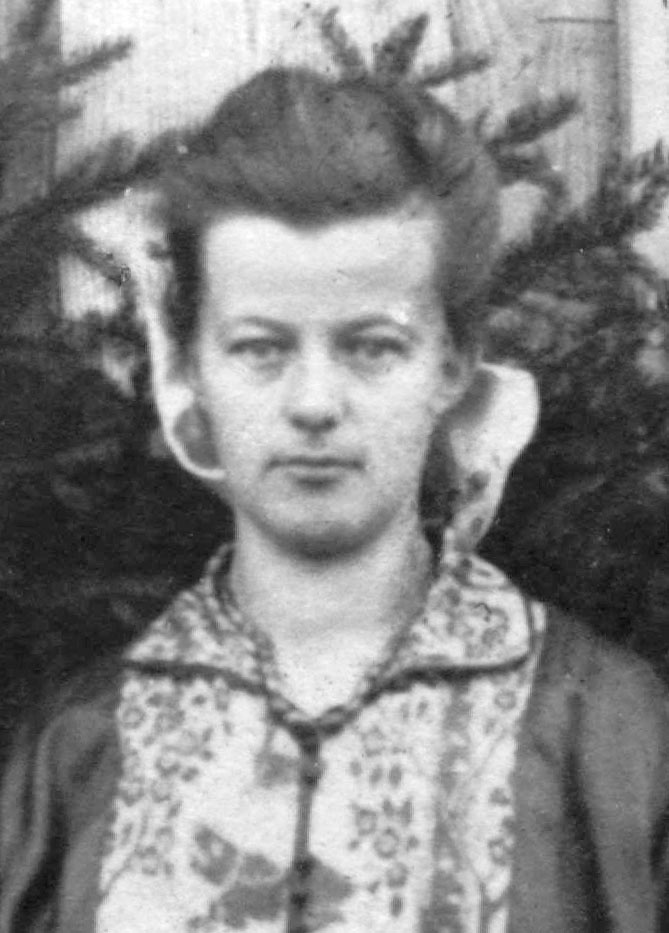
\includegraphics[width=4.3cm,height=5.973cm]{pictures/zulassungsarbeit-img039.jpg}

\end{center}
Theres Raster\\
\end{supertabular}
\end{flushleft}
Dass der Zustrom von neuen Sängerinnen und Sängern ausblieb, lag sicher
auch an dem Verhalten der Hauptsängerinnen. Sie hatten hauptsächlich
aus einem bestimmten Grund kein Interesse an einem größeren Chor:
Geld. \footnote{Interview Nr. 24, Johann Glasschröder, 28.12.2004,
Absatz 46} Denn je mehr Personen im Chor mitgesungen hätten, desto
öfter wäre die finanzielle Entschädigung, die dem Hauptchor zustand
aufzuteilen gewesen. Diese war etwa genau so hoch wie die des
Chorregenten. \footnote{Dokument Nr. 137, Chorabrechnung Ämter und
Messen, 3. Quartal 1952; Dokument Nr. 136, Chorabrechnung Beerdigungen
und Trauungen, 3. Quartal 1952; Dokument Nr. 138, Chorabrechnung, 4.
Quartal 1946} Das „Gehalt“ der einzelnen Sängerinnen wäre somit immer
kleiner ausgefallen. Aus dieser Sichtweise ist zum Beispiel das
Verhalten der Sängerin Theres Raster gegenüber neuen Chormitgliedern
durchaus nachvollziehbar. Raster war für den Notenschrank zuständig und
bestimmte sogar öfter als Högn, welches Stück gesungen werden
sollte. \footnote{Interview Nr. 2, Barbara Essigmann, 27.12.2002,
Absatz 94} Waren zu wenige Singstimmen vorhanden, und das war bei den
meist handgeschriebenen Notenmaterialien oft der Fall, gab sie
insbesondere den jungen Sängerinnen kein Notenblatt.\footnote{
Interview Nr. 16, Maria Freisinger, 25.8.2004, Absatz 8} Neue
Chormitglieder fühlten sich logischerweise weniger akzeptiert, wenn sie
wiederholt kein Notenblatt bekamen, noch dazu wenn ihnen nicht
klargemacht wurde, warum sie keine Stimmestimme bekommen
hatten. \footnote{Interview Nr. 16, Maria Freisinger, 25.8.2004, Absatz
12}

Der Hauptgrund, weshalb der Chor der Nachkriegszeit so wenige Mitglieder
zählte, ist aber in der Person von August Högn zu sehen. Mit 70 Jahren
hatte er nicht mehr den Elan, neue Sänger zu integrieren oder sich dem
intriganten Verhalten der Hauptsängerinnen entgegen zu
stellen. \footnote{Interview Nr. 16, Maria Freisinger, 25.8.2004,
Absatz 12} Vielleicht hat sich nicht nur sein hohes Alter, sondern auch
die Tatsache, dass er zeitlebens den Chorregentendienst nur
provisorisch oder aushilfsweise, paradoxerweise aber fast 20 Jahre lang
ausübte, wie in jedem Protokoll ausdrücklich erwähnt wird, und immer
nur als „Notnagel“ angesehen wurde, auf seine Einsatzbereitschaft
negativ ausgewirkt. Seinen drei großen heimatkundlichen Abhandlungen,
die alle in der Nachkriegszeit entstanden sind, entnimmt man, dass Högn
ab 1945 sein Hauptbetätigungsfeld nicht mehr in der Kirchenmusik sah.

\subsection{Heimatforschung als Betätigungsfeld im Ruhestand}

Die Heimatkunde: Ein Hobby des
Pensionisten Högn? Nach Eintritt ins Rentenalter verfasste Högn drei
Geschichten mit heimatkundlichem Inhalt. Die lockere Abfolge ihrer
Entstehung vermittelt den Eindruck, dass sie eher unter einem Zustand
der Ablenkung, des Zeitvertreibs beziehungsweise der Zerstreuung
entstanden sind. Dies trifft bei Högn nur teilweise zu. Seine
schriftstellerische Tätigkeit kann auch mit der Vollendung einer von
der Gesellschaft an die Lehrer übertragenen Aufgabe umschrieben werden.

Eine Aktion der Regierung von Niederbayern zur Zeit der Weimarer
Republik mit dem Motto \zitat{„Pflege des
Heimatgedankens“}, \footnote{Dokument Nr. 133, Regierungsblatt zur
Pflege des Heimatgedankens, 12.11.1925} hatte das Ziel, durch
Heimatkunde, den Patriotismus und das Nationalbewusstsein der Bürger zu
stärken, um damit einen Beitrag zur Lösung der nationalen Probleme zu
leisten. Ein Rundschreiben vom 12.11.1925, das auch Högn vorlag, mit
dem Betreff \zitat{„Anlegung gemeindlicher Ortsgeschichten“}
macht die Intention dieser Aktion in wenigen Sätzen deutlich:
\zitat{„Die Voraussetzung für den Aufstieg unseres Volkes aus
dem jetzigen Tiefstande ist die Rückkehr zu deutscher Einfachheit,
Zucht und Sitte. Dazu muss der Sinn für die Heimaterde geweckt“} und
\zitat{„die Liebe zum Vaterlande entzündet [...] werden. Auf
diesen }\zitat{Grundlagen baut sich neben der körperlichen
und geistigen Ertüchtigung der Jugend die Zukunft des deutschen Reiches
auf.“} Vor allem \zitat{„die Herren Lehrer [...] sollten“
}daher\zitat{ „ohne weiteres Säumen und mit allem Nachdruck
[...] die Vorbereitung für die Herstellung der
Ortsgeschichten“} \footnote{Dokument Nr. 133, Regierungsblatt zur
Pflege des Heimatgedankens, 12.11.1925} aufnehmen. Dass die
angetragenen Vorhaben eine gewisse Verbindlichkeit hatten, zeigt schon
die Aufforderung, dass \zitat{„bis zum 1. April 1928
berichtet werden wolle, [...] in welchen Gemeinden die Vorarbeiten in
Angriff genommen worden sind (Anrede des Bearbeiters).“ }\footnote{
Dokument Nr. 133, Regierungsblatt zur Pflege des Heimatgedankens,
12.11.1925} Högn hat sich tatsächlich dieser Aufgabe angenommen, wie
die vielen heimatkundlichen Zeitungsartikel zeigen, die in der Zeit von
1926 bis 1928 erschienen sind. Doch es waren nur einzelne
heimatkundliche Beiträge, die entstanden sind. Die eigentlich
geforderte komplette Ortsgeschichte blieb aus. Stand der Vollendung
dieser Aufgabe die Zeitknappheit aufgrund des Schuldienstes in Wege, so
beseitigte seine Pensionierung dieses Hindernis zur umfassenden
Ortsgeschichte. \footnote{Dokument Nr. 133, Regierungsblatt zur Pflege
des Heimatgedankens, 12.11.1925} Bei der Geschichte von Zachenberg
etwa, gibt es ganz konkrete Anhaltspunkte, wonach die Initiative zur
Inangriffnahme der Arbeit nicht von Högn selbst aus ging, für den
Begriff Hobby ein notwendiges Merkmal, sondern eine an ihn
herangetragene Bitte den Grund für die Entstehung der Geschichte
lieferte.

\begin{flushleft}
\tablefirsthead{}
\tablehead{}
\tabletail{}
\tablelasttail{}
\begin{supertabular}{m{5.2310004cm}}

\begin{center}

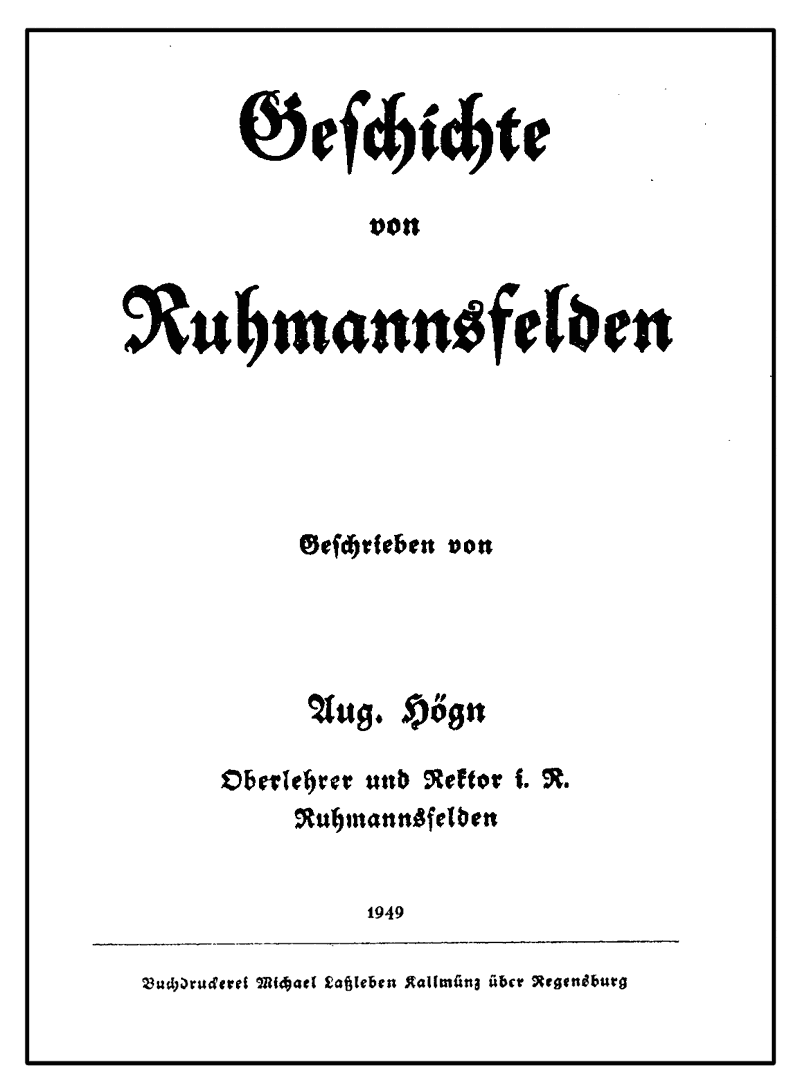
\includegraphics[width=4.995cm,height=6.833cm]{pictures/zulassungsarbeit-img040.png}

\end{center}
erste Seite der Geschichte von
Ruhmannsfelden\\
\end{supertabular}
\end{flushleft}

\begin{figure}
\img{}
\caption{}
\end{figure}

Gerade mal zwei Jahre nach Högns endgültiger Pensionierung,\footnote{
Dokument Nr. 48, Zeitungsartikel aus Viechtacher Bayerwald-Bote,
2.8.1958} erschien 1949 die „Geschichte von Ruhmannsfelden.“ Dem
rüstigen Rentner musste es eher leicht gefallen sein, Material für
seine Arbeit zu finden, konnte er doch auf eine rege Forschertätigkeit
vergangener Jahrzehnte zurückblicken und brauchte die vielen bereits
existierenden Einzelbeiträge zur Heimatgeschichte nur noch in einem
Werk zusammenfassen. Die geschichtliche Entwicklung zwei wichtiger
Institutionen am Ort hatte Högn lange vor dem 2. Weltkrieg bearbeitet:
Die Entwicklung der Ruhmannsfeldener Schule war in einer Beilage zum
Deggendorfer Donauboten 1927 erschienen und anlässlich der 100-jährigen
Einweihungsfeier der Ruhmannsfeldener Pfarrkirche wurde 1928 bis 1929
in mehreren Teilen die Geschichte der Pfarrkirche St. Laurentius im
Viechtacher Tagblatt abgedruckt. Information über die Entstehung des
Namens „Ruhmannsfelden“ oder den Zeitpunkt der Marktrechtsverleihung
beinhalteten zwei Zeitungsartikel aus dem Jahre 1926 und fanden an
exponierter Stelle Eingang in die „Geschichte von Ruhmannsfelden“. Es
war August Högn, der sich zur Frage des Namensursprungs von
„Ruhmannsfelden“ schon 1922 an den Straubinger Historiker Dr. Joseph
Keim wandte \footnote{Dokument Nr. 20, Brief von Dr. Keim an August
Högn, 30.8.1922} und die noch heute gültige Erklärung gab, wonach
Ruhmannsfelden nach dem Rodungsarbeiter „Rumar“ benannt wurde. Davor
wurde der Name „Ruhmannsfelden“ etwas trivial mit „Ruht der Mann in
Felde“ erklärt. \footnote{Interview Nr. 9, Dr. Doraliesa Wiegmann,
19.1.2003, Absatz 4} Ebenso versuchte Högn sowohl in dem erwähnten
Artikel als auch in der „Geschichte von Ruhmannsfelden“ dem Mythos,
dass einst ein Schloss am Leitenberg bestand, entgegenzuwirken. Trotz
aller realisierbaren Recherchearbeiten ist es unverkennbar, dass Högn
besonders zur frühen Geschichte Ruhmannsfeldens auf sehr wenige
Informationen zurückgreifen konnte. Das einleitende Kapitel der
Geschichte von Ruhmannsfelden „Wie hat es vor seiner Entstehung
ausgesehen?“ ähnelt in seinem Aufbau mehr einem Roman als dem Beginn
einer historischen Abhandlung und entbehrt sicherlich aller
wissenschaftlichen Beweise. Wegen fehlender Dokumente musste von Namen
wie etwa „Ruhmannsfelden“ oder „Laurentius-Kirche“ auf die mögliche
geschichtliche Entwicklung geschlossen werden. Manchmal schlussfolgerte
Högn aus diesen Anhaltspunkten etwas zuviel. Es stimmt sicher, dass
alle dem hl. Laurentius geweihten Kirchen außerhalb der Ortschaften
standen, aber dass die „Laurentius“-Kirche in Ruhmannsfelden zuerst aus
Holz war, unter den Aldersbachern dann aus Stein und dass dann auch
öfter Gottesdienste stattfanden, wie in der Geschichte von
Ruhmannsfelden steht, ist wohl rein Spekulation. \footnote{Högn,
Ruhmannsfelden, Seite 10} Als Lückenfüller dürften die Kapitel über die
Namen der Ruhmannsfeldener Fluren und Gassen und eine Auflistung der
Höhenlagen mit Barometerstand der umliegenden Berge und Ortschaften
gedient haben.

Der Entstehungsgrund der „Geschichte und Chronik der freiwilligen
Feuerwehr Ruhmannsfelden“ ist eng mit dem Ende von Högns
Schriftführertätigkeit bei der Feuerwehr verbunden. Am Stefani-Tag 1950
wurde Johann Freisinger zum Schriftführer der Feuerwehr Ruhmannsfelden
gewählt und löste somit August Högn nach 40-jähriger Dienstzeit ab. Die
\zitat{„in dankbarer Erinnerung“}  \footnote{Högn,
Ruhmannsfelden, Titelblatt} der Feuerwehr gewidmete Geschichte hat Högn
geschrieben, um seine Tätigkeit als Schriftführer abzurunden und sein
in 40 Jahren gesammeltes Wissen in diese Arbeit einfließen zu lassen.
Ein passender Übergabetermin der Chronik an die Feuerwehr wäre der zur
Verabschiedung von Högn eigens veranstaltete Ehrenabend am 11. März
1951 gewesen, doch die Chronik wurde der letzten Eintragung zufolge
erst nach dem 1. April 1951 fertig geschrieben. Aber die Arbeit war zum
Ehrenabend der Feuerwehr schon versprochen und fand deswegen lobende
Erwähnung in der Abschiedesrede des Feuerwehrkommandanten.\footnote{
Dokument Nr. 110, Abschiedsrede des Feuerwehrkommandanten Johann
Linsmeier, 3.11.1951} Die fertige Chronik überreichte Högn persönlich
dann kurze Zeit später seinem Schriftführer-Nachfolger.\footnote{
Interview Nr. 14, Johann Freisinger, 29.12.2003, Absatz 16} Die
Abhandlung ist nach Jahrgängen gegliedert und lässt daher oft
Einzelfakten unverbunden nebeneinander stehen, was das Verständnis beim
Lesen erschwert. Sie ist deshalb wohl eher als eine Stoffsammlung zur
weiteren Bearbeitung anzusehen, als ein unterhaltsamer Lesestoff für
die breite Ruhmannsfeldener Bevölkerung und war sicher nie für den
Druck bestimmt. Lediglich die länger ausformulierte Gründung der
Feuerwehr und der Bericht samt Querverweisen über den sich über
längeren Zeitraum erstreckende und deshalb in mehreren Jahren
auftauchende Streit der Gemeinden Ruhmannsfelden und Zachenberg um eine
gemeinsam angeschaffte Feuerwehrspritze bleiben dem Leser in Erinnerung
und gehen nicht in der Flut von Einzelinformationen unter.

\begin{center}
\begin{minipage}{10.007cm}
\begin{flushleft}
\tablefirsthead{}
\tablehead{}
\tabletail{}
\tablelasttail{}
\begin{supertabular}{m{5.0280004cm}m{4.578cm}}

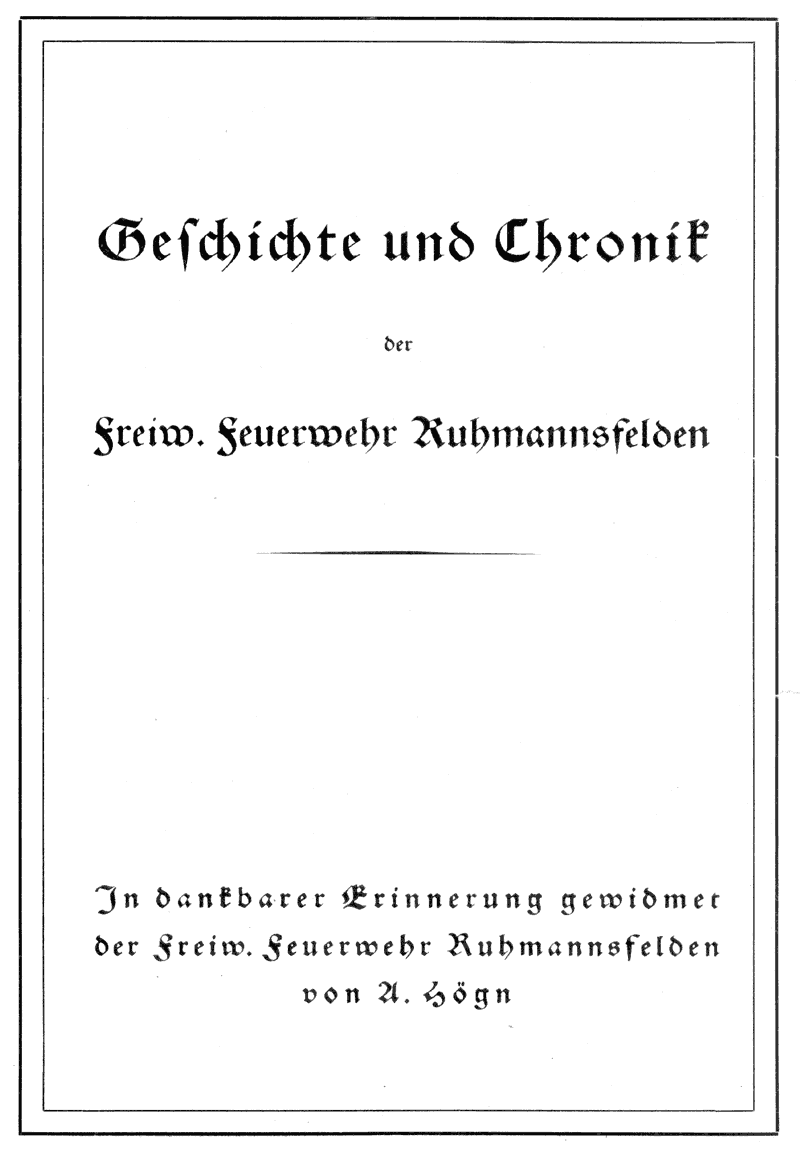
\includegraphics[width=4.847cm,height=6.997cm]{pictures/zulassungsarbeit-img041.png}

Deckblatt des Manuskripts der
„Geschichte und Chronik der Freiw. Feuerwehr Ruhmannsfelden“ &

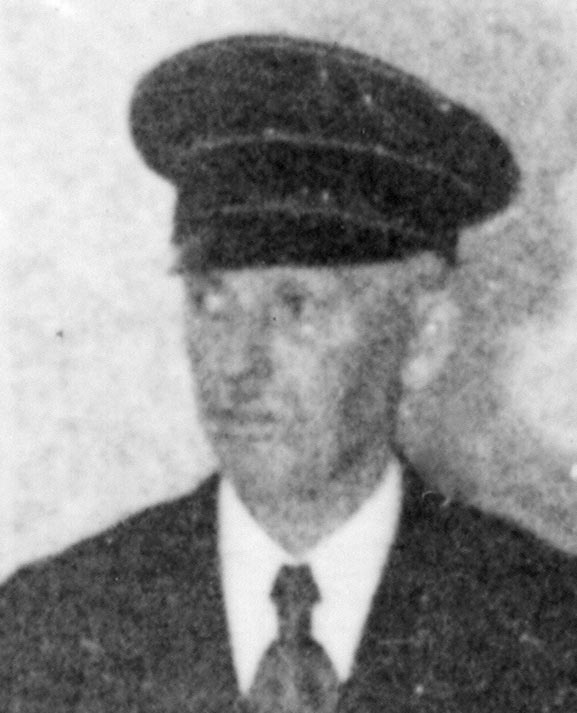
\includegraphics[width=4.396cm,height=6.997cm]{pictures/zulassungsarbeit-img042.jpg}

August Högn bei der Mitglieder-Ehrung
der Feuerwehr 1950\\
\end{supertabular}
\end{flushleft}
\end{minipage}
\end{center}

\begin{figure}
\img{}
\caption{}
\end{figure}

Ein auswärtiger, nicht in der Gemeinde Zachenberg ansässiger Bürger
lieferte die Initiative zur Entstehung von Högns „Heimat-Geschichte der
Gemeinde Zachenberg.“ Der Finanzzollrat Anton Trellinger – er war am
Landshuter Hauptstaatsarchiv als Archivpfleger angestellt – fertigte
einen 63-seitigen Akten-Auszug \footnote{Dokument Nr. 31, Brief von
August Högn an Klosterbibliothekar des Klosters Niederalteich,
26.3.1952, Dokument Nr. 33, Brief von August Högn an das Pfarramt
Grafenau, 26.3.1952} über die Gemeinde Zachenberg an. Da Trellinger die
Gemeinde Zachenberg nur flüchtig kannte und gesundheitlich sehr
angeschlagen war, \footnote{Dokument Nr. 28, Brief von Finanzzollrat
Anton Trellinger an August Högn, 25.2.1952} – er erlitt im Frühjahr
1952 einen Schlaganfall \footnote{Dokument Nr. 35, Brief von Expositus
Georg Hofmann, Schönau an August Högn, 23.10.1952} – bat er seinem
Brief die Gemeinde Zachenberg um einen ortskundigen Fachmann, der seine
Arbeit ergänzen und fortführen könnte. Den Sachbearbeitern bei der
Gemeinde dürfte es nicht schwer gefallen sein, Trellinger die
geforderte Person zu nennen: August Högn. Lange bevor Anton Trellinger
der Gemeinde Zachenberg seine Arbeit übersandte, nämlich am 25.2.1952,
und am selben Tag Högn persönlich anschrieb, \footnote{Dokument Nr. 28,
Brief von Finanzzollrat Anton Trellinger an August Högn, 25.2.1952}
hatte August Högn schon mit der Recherche begonnen und den Mettener
Benediktiner-Pater Wilhelm Fink von der beabsichtigen Geschichte von
Zachenberg in Kenntnis gesetzt und um wissenschaftliche Betreuung
gebeten. \footnote{Dokument Nr. 29, Brief von Pater Wilhelm Fink an
August Högn, 28.1.1952}

\begin{center}
\begin{minipage}{5.378cm}
\begin{flushleft}
\tablefirsthead{}
\tablehead{}
\tabletail{}
\tablelasttail{}
\begin{supertabular}{m{5.178cm}}

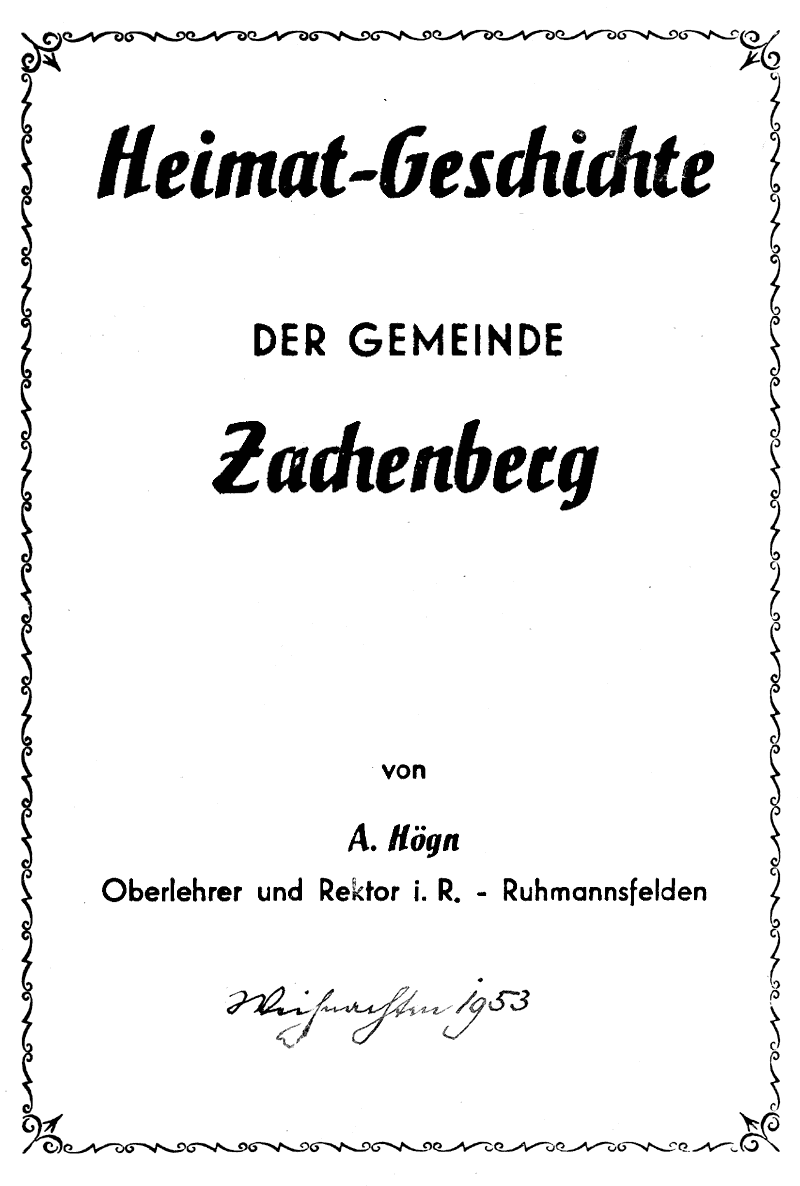
\includegraphics[width=4.995cm,height=7.405cm]{pictures/zulassungsarbeit-img043.png}

Deckblatt des Manuskripts der
„Heimat-Geschichte der Gemeinde Zachenberg“\\
\end{supertabular}
\end{flushleft}
\end{minipage}
\end{center}
Trellinger lieferte mit seinen Archivauszügen nicht nur einen wichtigen
Grundstock für Högns „Heimat-Geschichte der Gemeinde Zachenberg“,
sondern er gab ihm auch einige Tipps und Literaturhinweise.\footnote{
Dokument Nr. 28, Brief von Finanzzollrat Anton Trellinger an August
Högn, 25.2.1952} Nach fast 2-jähriger Arbeitszeit wurde die „Geschichte
von Zachenberg“ an Weihnachten 1953 fertig gestellt \footnote{Högn,
Zachenberg, Deckblatt} und an Wilhelm Fink zum Korrekturlesen
übersandt. Fink hatte besonders zum 1. Teil der Abhandlung einige
Änderungsvorschläge anzubieten. Es ist deshalb nicht verwunderlich,
dass sich die ersten Teile der „Geschichte von Ruhmannsfelden“ und der
„Geschichte von Zachenberg“ im Aufbau und in der Darstellung ziemlich
stark unterscheiden, obwohl beide Teile die geschichtliche Entwicklung
von den Anfängen der beiden benachbarten und sich unter den gleichen
Herrschaftsverhältnissen entwickelnden Gemeinden zum Thema haben. Fink
hat offensichtlich die „Geschichte von Ruhmannsfelden“ nicht Korrektur
gelesen. Im von Fink als druckreif befunden 2. Teil der Geschichte von
Zachenberg geht Högn auf die 15 Dörfer, 13 Weiler und 10 Einöde, also
auf die insgesamt 38 Ortschaften der Gemeinde Zachenberg im Einzelnen
ein.

Die Kapitel über die einzelnen Ortschaften ähneln mehr genealogischen
Studien als historischen Abhandlungen. Manchmal lassen sich aus diesen
Kapiteln Stammbäume einzelner Bauernfamilien über Jahrhunderte hinweg
ablesen. Meistens jedoch konnten die Angaben aus den sehr alten
Aktenauszügen Trellingers nicht mit den neueren Informationen aus dem
Gemeindearchiv oder von den befragten Bewohnern der jeweiligen
Ortschaft bruchlos aneinander gereiht werden. Die sehr schematische
Beschreibung der kleinsten Ortschaften selbst – sie beginnt immer mit
der Herkunfts-Erklärung des Ortsnamens und endet nach Vorstellung der
einzelnen Bauernfamilien mit Angabe der damals aktuellen Einwohner- und
Häuserzahl – wird durch Sagen und Erzählungen aufgelockert, die Högn
von älteren Bewohnern der einzelnen Orte erzählt bekam und sie in Form
von Nacherzählungen wiedergibt. Viele der von Wilhelm Fink
vorgeschlagenen Ergänzungen zum dritten, allgemeinen Teil – hier geht
es in erster Linie um die damalige aktuelle Organisation der Gemeinde –
hat Högn nicht angenommen, weil beiden Gemeinden, Zachenberg und
Ruhmannsfelden, doch sehr ähnliche Strukturen aufwiesen und er bereits
Einiges in der Geschichte von Ruhmannsfelden erwähnt hatte, wie zum
Beispiel die aus der Pfarrei hervorgegangenen Priester, die Lehrer oder
die Polizei. Deshalb erörtert er hier hauptsächlich die aktuellen
wirtschaftlichen und infrastrukturellen Aspekte der Gemeinde
Zachenberg. \footnote{Dokument Nr. 38, Brief von Pater Wilhelm Fink,
Metten an August Högn, 23.2.1954}

Als er die korrigierte Fassung der Geschichte kurz vor Ostern 1954 der
Gemeinde Zachenberg übergab, rechnete er sicher mit einer schnellen
Drucklegung seiner Arbeit, ähnlich wie bei der Geschichte von
Ruhmannsfelden, sonst hätte er sich nicht schon von der Druckerei
Michael Laßleben in Kallmünz ein Angebot geben lassen und sich sogar
schon einen Werbetext für ein Inserat oder ein Plakat
überlegt. \footnote{Dokument Nr. 39, Brief von August Högn an
Bürgermeister Ludwig Bielmeier, Zachenberg, 31.3.1954}

\begin{center}
\begin{minipage}{5.812cm}
\begin{center}
\tablefirsthead{}
\tablehead{}
\tabletail{}
\tablelasttail{}
\begin{supertabular}{m{5.612cm}}

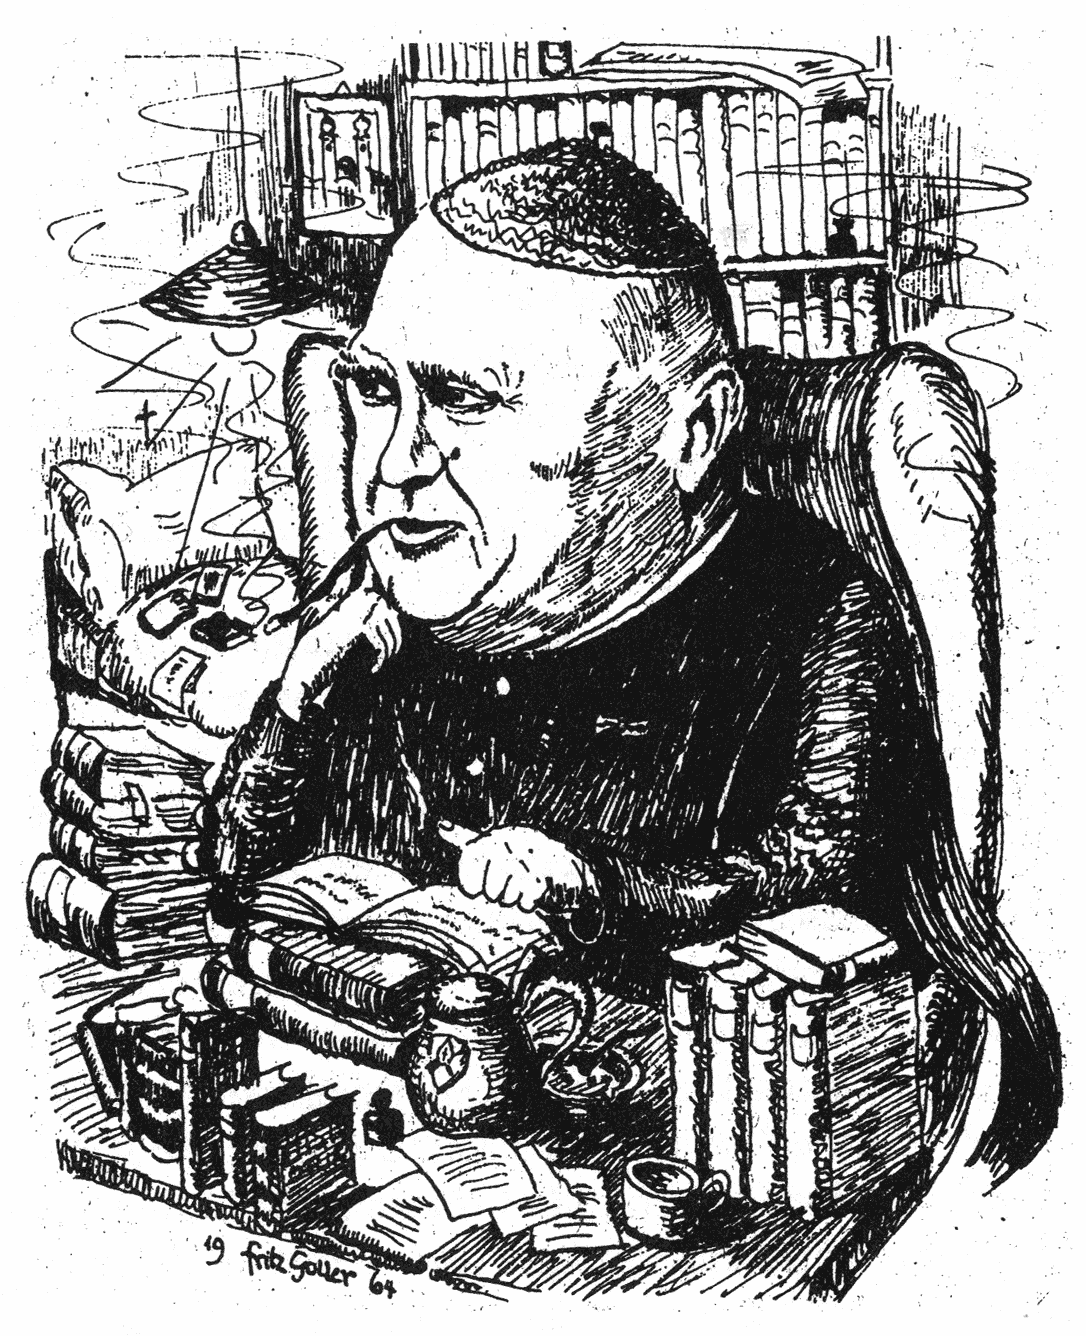
\includegraphics[width=5.429cm,height=6.68cm]{pictures/zulassungsarbeit-img044.png}

Wilhelm Fink in einer Karikatur von
Fritz Goller\\
\end{supertabular}
\end{center}
\end{minipage}
\end{center}

\begin{figure}
\img{}
\caption{}
\end{figure}

Erst am 7. Mai 1956 versicherte der Zachenberger Bürgermeister Bielmeier
August Högn, auf seine Anfrage hin, dass der Gemeinderat über die
Veröffentlichung der „Geschichte von Zachenberg“ in der nächsten
Sitzung beraten würde. \footnote{Dokument Nr. 40, Brief von
Bürgermeister Ludwig Bielmeier, Zachenberg an August Högn, 7.5.1956}
Die Gemeindevorsteher hatten wohl von Anfang an kein Interesse an einer
Drucklegung. \footnote{Interview Nr. 14, Johann Freisinger, 29.12.2003,
Absatz 13 – 14} Kein einziges Wort ist über den Druck des Buchs im
Protokoll der Gemeinderatssitzung vom 17.5.1956 zu finden. Stattdessen
wurde beschlossen, Högn zum Ehrenbürger der Gemeinde Zachenberg zu
ernennen und ihm als \zitat{„Entschädigung“ }für seine
Bemühungen ein \zitat{„Geldgeschenk im Ermessen des 1.
Bürgermeisters“} \footnote{Dokument Nr. 96,
Sitzungsprotokoll des Gemeinderats Zachenberg, 17.5.1956} zukommen zu
lassen. Trotz aller dieser Ehren dürfte die immer noch nicht
eingeleitete Vervielfältigung der „Geschichte von Zachenberg“ eine
Enttäuschung für Högn gewesen sein. Noch an seinem 80. Geburtstag, also
über 4 Jahre nach der Fertigstellung des Werks, machte er sich Hoffnung
auf eine baldige Drucklegung des Werks, \footnote{Dokument Nr. 48,
Zeitungsartikel aus Viechtacher Bayerwald-Bote, 2.8.1958} die bis zum
heutigen Tag auf sich warten lässt.

\begin{flushleft}
\tablefirsthead{}
\tablehead{}
\tabletail{}
\tablelasttail{}
\begin{supertabular}{m{3.7879999cm}}

\begin{center}

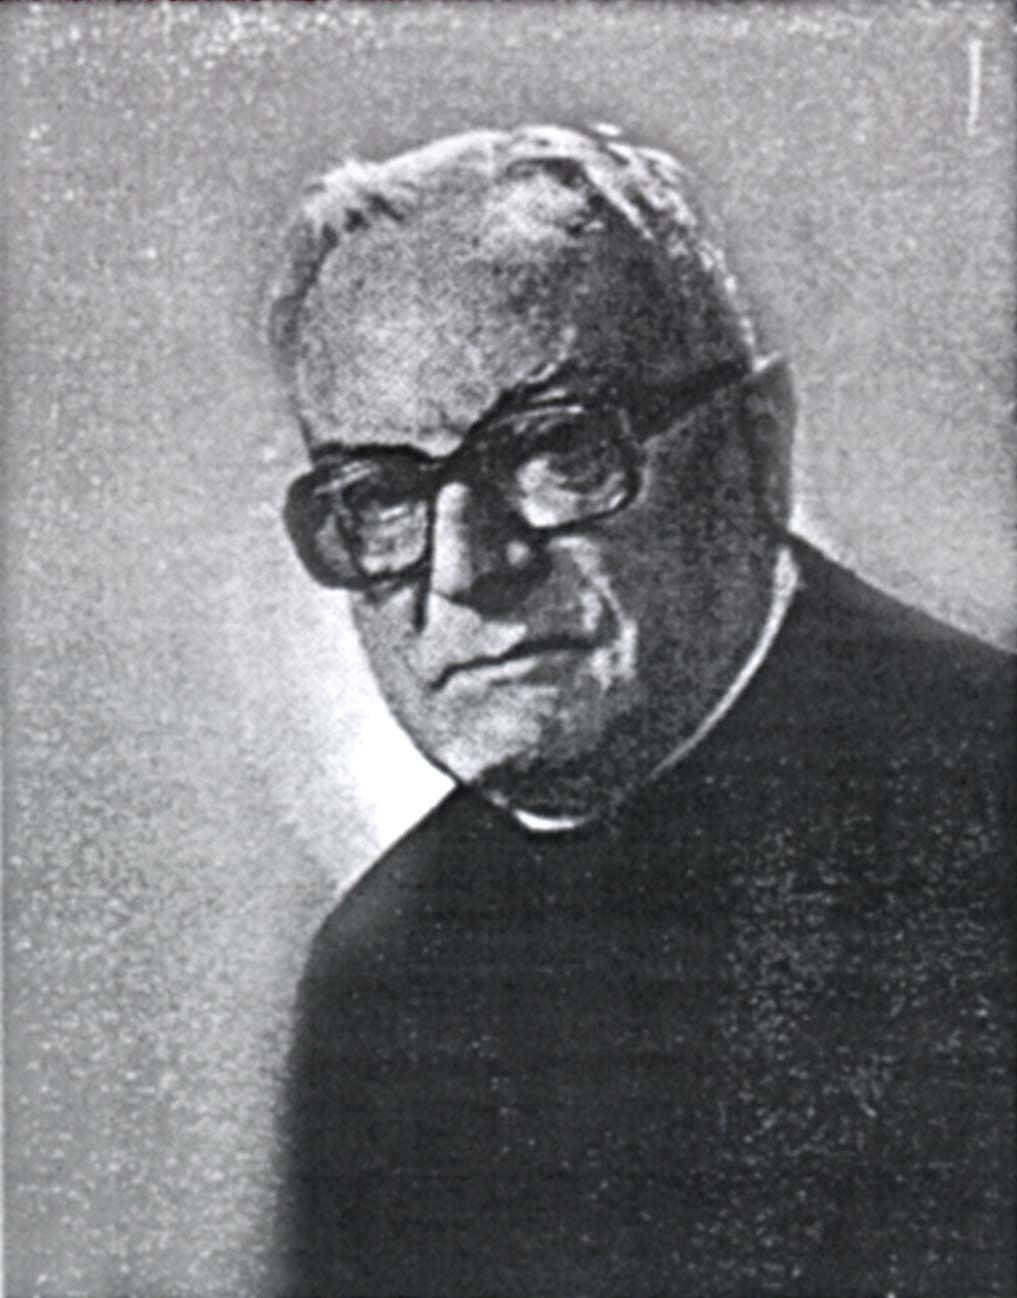
\includegraphics[width=3.605cm,height=4.6cm]{pictures/zulassungsarbeit-img045.jpg}

\end{center}
Ferdinand Haberl\\
\end{supertabular}
\end{flushleft}

\begin{figure}
\img{}
\caption{}
\end{figure}

August Högn war nicht nur auf heimatkundlichem Gebiet schriftstellerisch
tätig. Es gibt Anzeichen dafür, dass er sich auch mit musikhistorischen
Themen beschäftigt haben könnte. Ein Briefwechsel aus dem Jahr 1947 mit
Ferdinand Haberl, Direktor der Kirchenmusikschule in Regensburg, in dem
es um die Entstehung und Herkunft des Weihnachtsliedes „Stille Nacht“
geht, unterstreicht diese Annahme. \footnote{Dokument Nr. 65, Brief von
August Högn an Dr. Haberl, Regensburg, Mrz. 1947; Dokument Nr. 61,
Brief von F. Mitterwallner, Deggendorf an August Högn, 25.2.1947}

\subsection{Unwürdiger Abschied als Chorregent}

\hypertarget{RefHeadingToc100333737}{}Ähnlich große Wellen wie die
Entlassung des Chorregenten Max Rauscher im Jahr 1927 schlug 1953
August Högns Ausscheiden als Kirchenchorleiter. Dem Chorleiterwechsel
ging ein Pfarrerwechsel voraus. Am 17. Februar 1953 verstarb Pfarrer
Jakob Bauer. \footnote{Reicheneder-Chronik, Seelsorger, Blatt III/14
(4) Vorderseite} Der neue Pfarrherr Franz Seraph Reicheneder wurde am
26. Mai 1953 in Ruhmannsfelden empfangen und am 14. Juni\footnote{
Reicheneder-Chronik, Seelsorger, Blatt III/15 (1) Vorderseite}
schließlich feierlich mit Högns „Josephi“-Messe installiert.\footnote{
Dokument Nr. 41, Zeitungsartikel aus dem Viechtacher Bayerwald-Boten,
15.6.1953} August Högn wollte eigentlich bei Antritt des neuen Pfarrers
seinen Rücktritt als Chorregent und Organist bekannt geben, doch der
neue Pfarrer lehnte sein Ersuchen anstandsgemäß ebenso wie vor einiger
Zeit Pfarrer Jakob Bauer und in der Übergangszeit Pfarrprovisor Georg
Huber ab. \footnote{Dokument Nr. 18, Brief von August Högn an Pfarrer
Reicheneder, 25.1.1954} August Högns Rücktrittsabsichten sprachen sich
sogar herum, sodass Josef Brunner – er war während der Kriegszeit
Aushilfsorganist in Ruhmannsfelden – eine Bewerbung für die
möglicherweise frei werdende Chorregentenstelle bei der
Kirchenverwaltung Ruhmannsfelden einreichte. \footnote{Dokument Nr. 17,
Brief von Josef Brunner an Kirchenverwaltung, 29.4.1953}

\begin{center}
\begin{minipage}{4.032cm}
\begin{flushleft}
\tablefirsthead{}
\tablehead{}
\tabletail{}
\tablelasttail{}
\begin{supertabular}{m{3.832cm}}

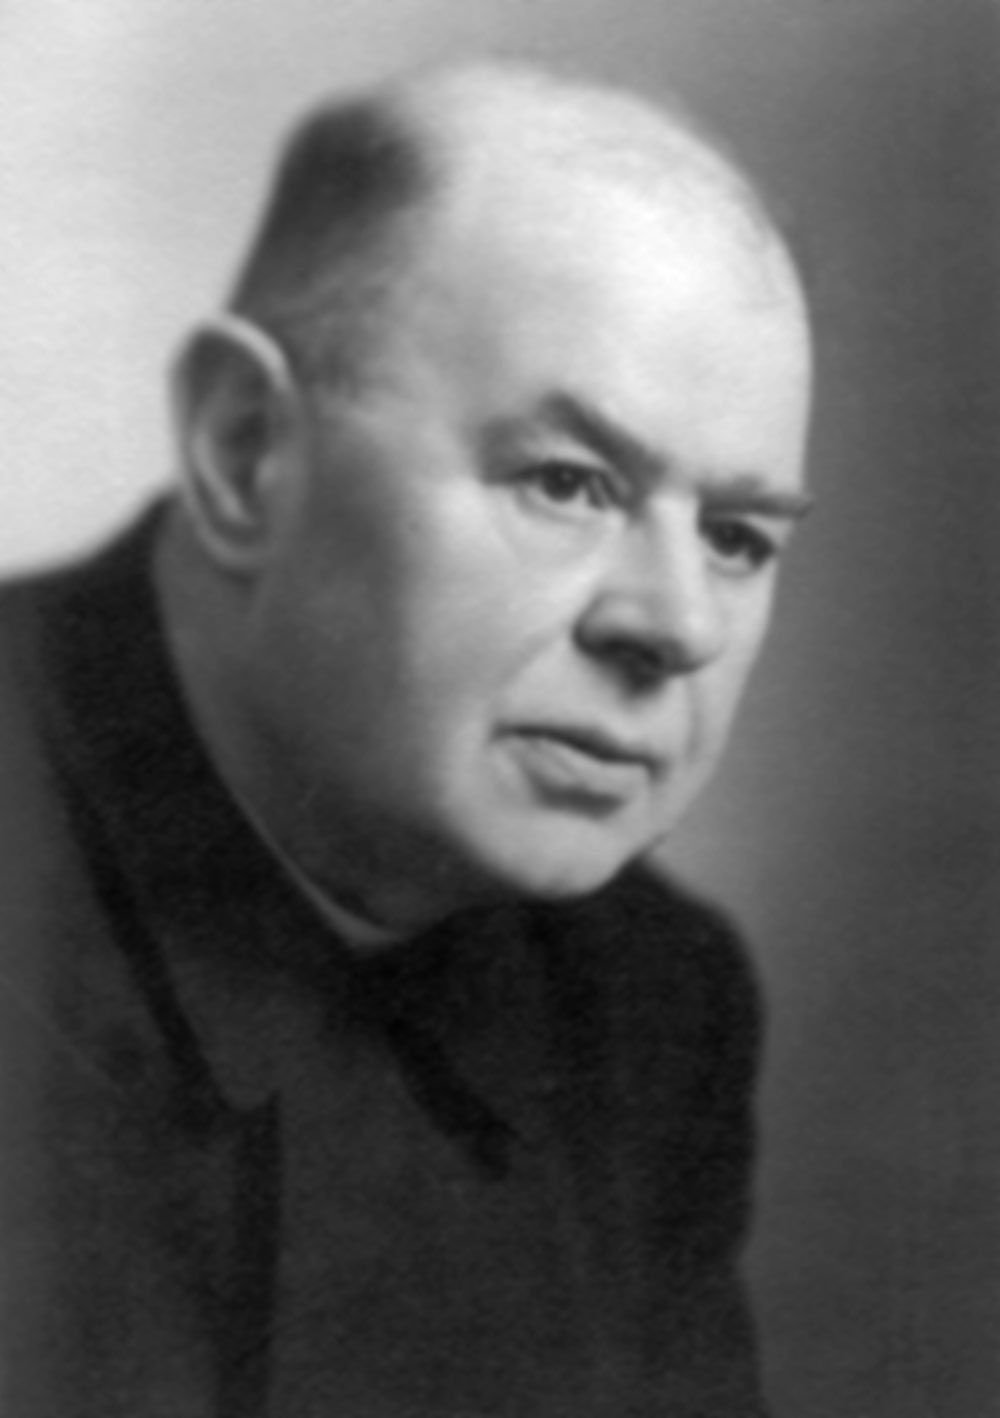
\includegraphics[width=3.651cm,height=5.177cm]{pictures/zulassungsarbeit-img046.jpg}

Abb. \stepcounter{Abb}{\theAbb}: Jakob Bauer\\
\end{supertabular}
\end{flushleft}
\end{minipage}
\end{center}
Umso verwunderlicher ist die Dramatik wie sich Högns Ausscheiden als
Chorregent dann tatsächlich vollzog: Nachdem Högns Bitte um Rücktritt
von Pfarrer Reicheneder abgelehnt wurde, scheint Högn weiterhin mit
einer längerfristigen Dienstzeit als Chorregent und Organist gerechnet
zu haben, sonst hätte er nicht schon 1953 zwei Marienlieder zum
marianischen Jahr 1954 komponiert. Reicheneder hingegen, von Högns
Amtsmüdigkeit überzeugt, war wahrscheinlich davon ausgegangen, dass der
75-jährige Högn bald abdankt würde. \footnote{Interview Nr. 24, Johann
Glasschröder, 28.12.2004, Absatz 48} Vielleicht hatte er auch schon
deswegen seiner von vorneherein favorisierter Nachfolgerin Maria
Reisinger eine baldige Anstellung in Aussicht gestellt. Maria
Reisinger, ein Waisenkind, war Reicheneders Ziehtochter, um deren
Ausbildung sich Reichender gekümmert hatte.

Mit Sicherheit hat Reicheneder die Ablehnung des Rücktrittsgesuchs aus
folgenden zwei Gründen bereut: Zum einem war für seine Ziehtochter
keine Anstellung in absehbarer Zeit greifbar, zum anderen leisteten zum
damaligem Zeitpunkt Högn und sein Chor äußerst schlechte Darbietungen.
Die Aufführung der „Josephi“-Messe durch den
\zitat{„klangvollen Chor“}
\footnote{Dokument Nr. 41, Zeitungsartikel aus dem Viechtacher
Bayerwald-Boten, 15.6.1953} zu Reicheneders Installation war nicht
repräsentativ für den alltäglichen Kirchenmusikbetrieb, da hier viele
Aushilfen mitwirkten \footnote{Interview Nr. 24, Johann Glasschröder,
28.12.2004, Absatz 44} und hatte möglicherweise bei Reicheneder ein
falschen Eindruck hinterlassen.

\begin{flushleft}
\tablefirsthead{}
\tablehead{}
\tabletail{}
\tablelasttail{}
\begin{supertabular}{m{3.5939999cm}m{4.361cm}m{4.123cm}m{3.3769999cm}}

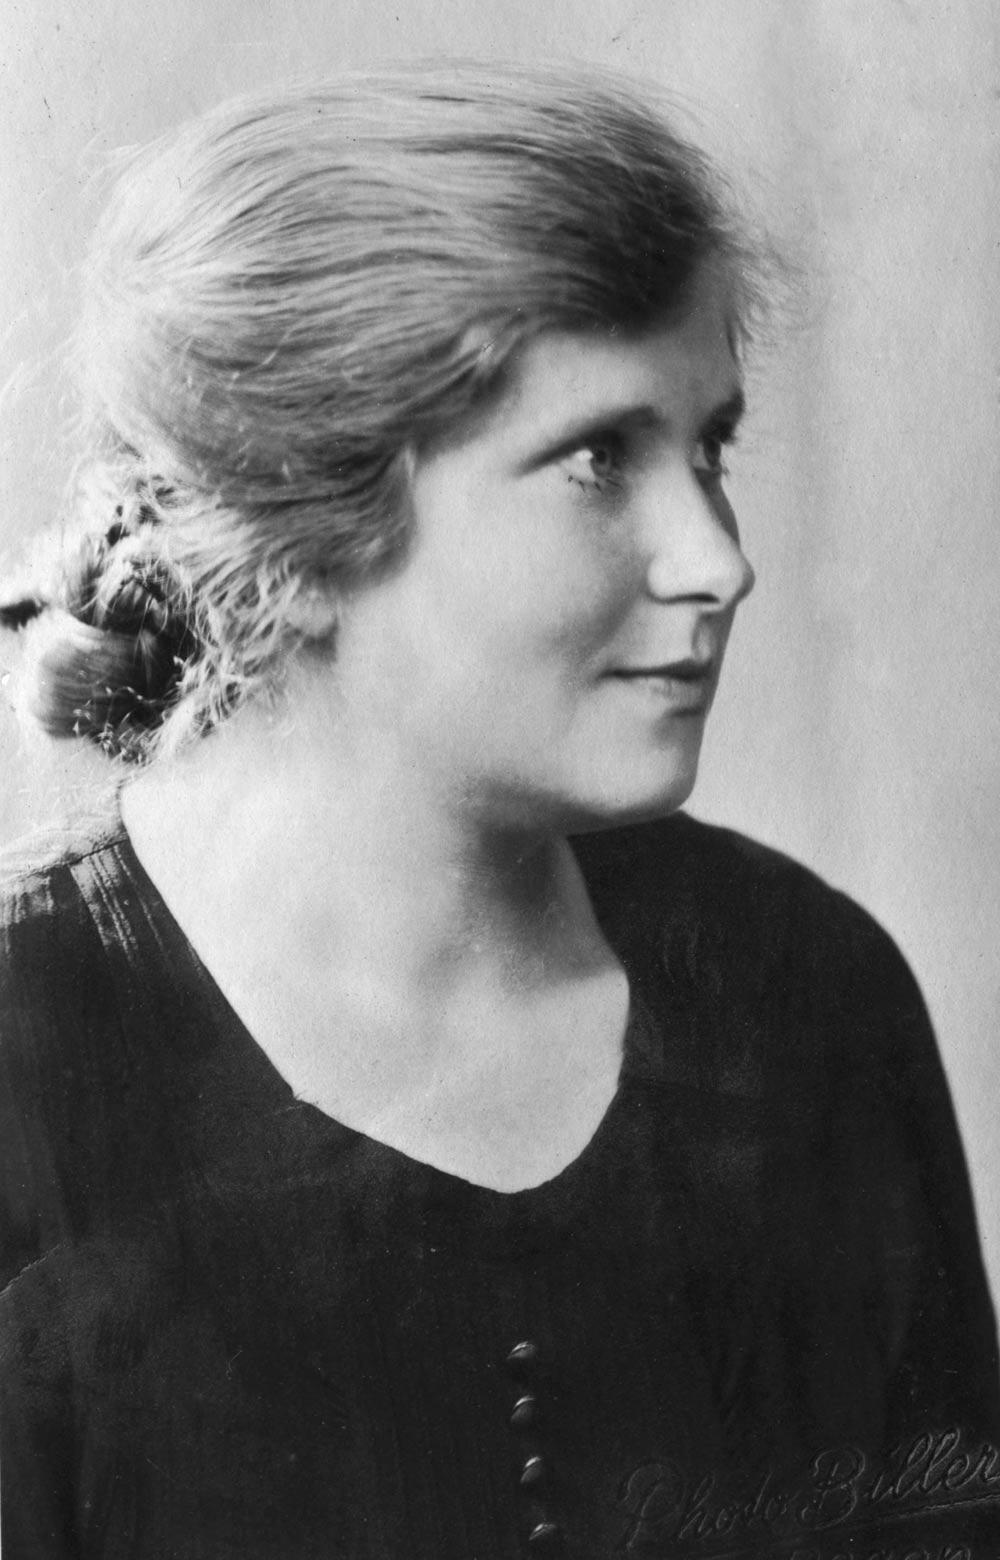
\includegraphics[width=3.413cm,height=5.323cm]{pictures/zulassungsarbeit-img047.jpg}

Abb. \stepcounter{Abb}{\theAbb}: Der „Chor“ der Nachkriegszeit: Mathilde
Glasschröder &

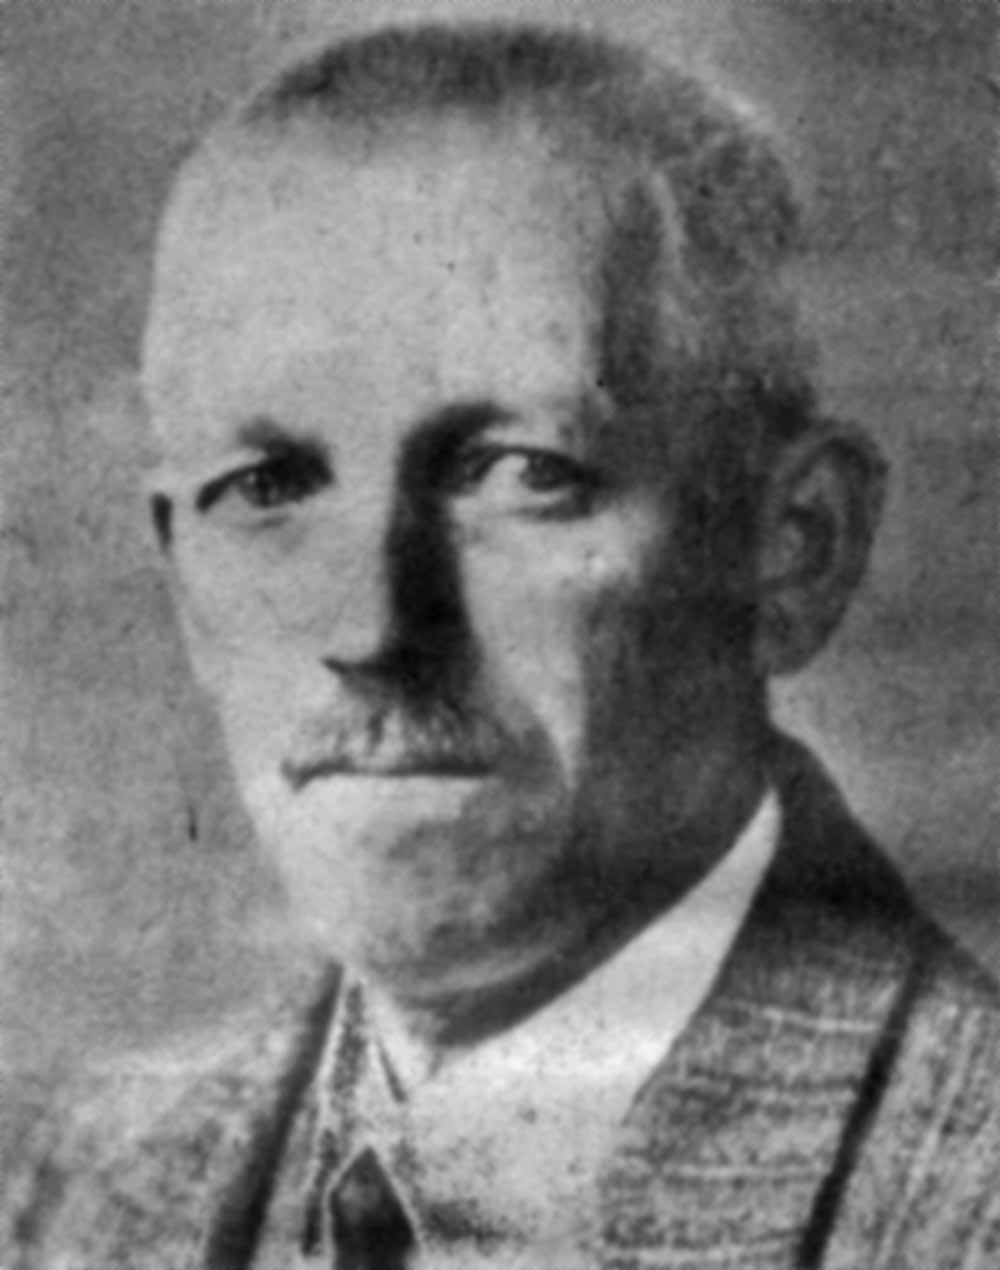
\includegraphics[width=4.18cm,height=5.308cm]{pictures/zulassungsarbeit-img048.jpg}

Abb. \stepcounter{Abb}{\theAbb}: August Högn &

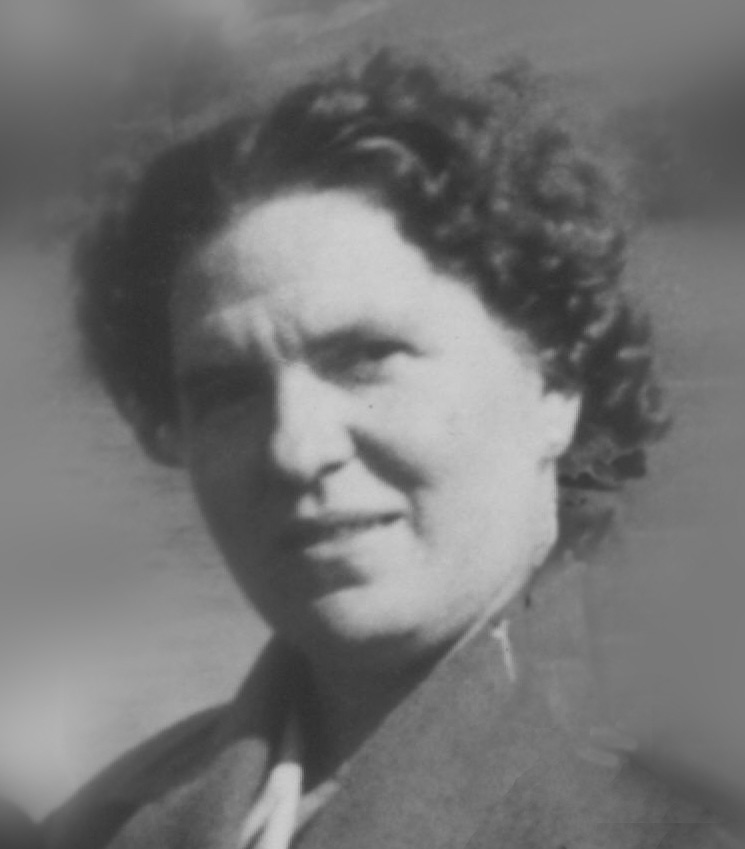
\includegraphics[width=3.942cm,height=5.3cm]{pictures/zulassungsarbeit-img049.jpg}

Abb. \stepcounter{Abb}{\theAbb}: Barbara Essigmann  &

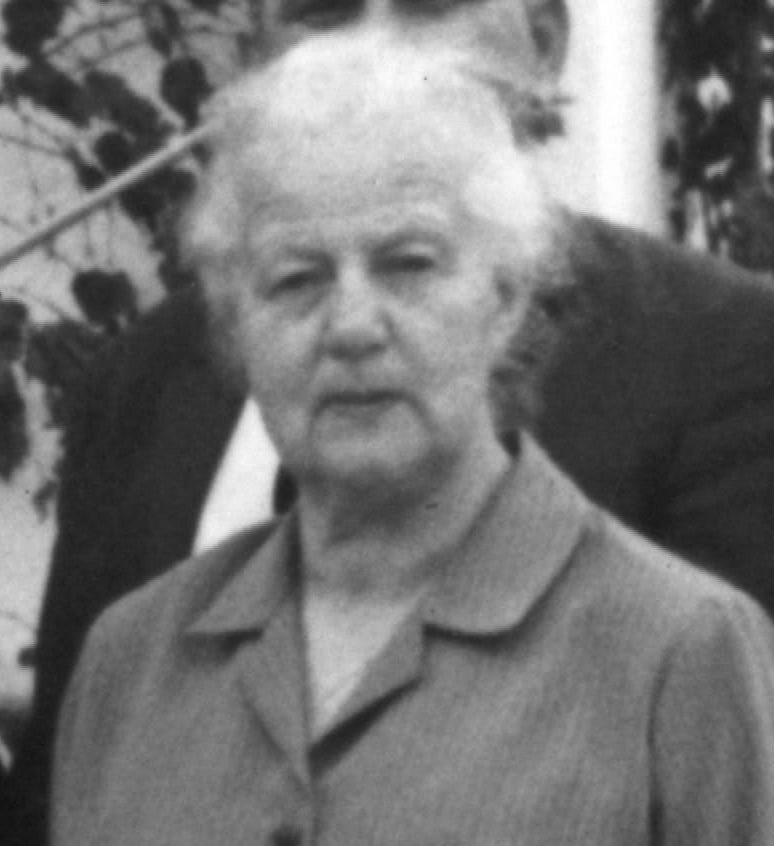
\includegraphics[width=3.194cm,height=5.281cm]{pictures/zulassungsarbeit-img050.jpg}

Abb. \stepcounter{Abb}{\theAbb}: Theres Raster\\
\end{supertabular}
\end{flushleft}
Der „Chor“, der unter der Woche sang, bestand nur aus vier Personen: Den
drei Sängerinnen Mathilde Glasschröder, Barbara Essigmann, Theres
Raster, und August Högn, der selbst eine Männerstimme
übernahm. \footnote{Interview Nr. 24, Johann Glasschröder, 28.12.2004,
Absatz 2} Vor allem die Heterogenität der einzelnen Stimmen
untereinander, die durch die Kleinstbesetzung unverdeckt hervortrat,
hinterließ bei so manchen Kirchenbesuchern einen schlechten
Eindruck. \footnote{Interview Nr. 9, Dr. Doraliesa Wiegmann, 19.1.2003,
Absatz 4; Interview Nr. 24, Johann Glasschröder, 28.12.2004, Absatz 36}
Wurde Mathilde Glasschröder als sängerische Naturbegabung mit großer
Stimme vergleichbar einer Opernsängerin beschrieben,\footnote{
Interview Nr. 13, Lorenz Schlagintweit, 29.11.2003, Absatz 2; Interview
Nr. 24, Johann Glasschröder, 28.12.2004, Absatz 52} blieb Theres Raster
als außerordentlich schlechte Sängerin mit „fürchterlichem“ Stimmklang
in Erinnerung. \footnote{Interview Nr. 24, Johann Glasschröder,
28.12.2004, Absatz 46} Die alternde Stimme Högns scheint sich ebenso
wenig in einen Gesamtklang eingebunden zu haben. \footnote{Interview
Nr. 24, Johann Glasschröder, 28.12.2004, Absatz 36} Neben dem
schlechtem Gesang stellte für Reicheneder möglicherweise das
kirchenmusikalische Repertoire einen Stein des Anstoßens dar. Ein und
dasselbe Lied, das zum Schluss des Gottesdienstes gesungen wurde, hatte
sich als „Standardstück“ eingebürgert \footnote{Interview Nr. 16, Maria
Freisinger, 25.8.2004, Absatz 20} und nicht nur werktags wurden Teile
aus dem Gloria und Credo übersprungen. \footnote{Interview Nr. 24,
Johann Glasschröder, 28.12.2004, Absatz 26; Interview Nr. 2, Barbara
Essigmann, 27.12.2002, Absatz 36; Interview Nr. 16, Maria Freisinger,
25.8.2004, Absatz 14}

Obwohl in Ruhmannsfelden die Bereitschaft zum Singen recht groß war – es
gab neben dem Kirchenchor einen Männerchor und eine weltliche
Liedertafel \footnote{Interview Nr. 24, Johann Glasschröder,
28.12.2004, Absatz 10, 4 } – gab es in Ruhmannsfelden lediglich ein
Gesangsquartett als Kirchenchor. Reicheneder muss als Hauptgrund für
diesen Missstand die laxe Probenpraxis in Högns Wohnung angesehen
haben, den er durch Ansetzung von öffentlichen Proben zu beseitigen
versuchte – wohl bemerkt mit Högn als Chorleiter. \footnote{Interview
Nr. 24, Johann Glasschröder, 28.12.2004, Absatz 43 – 44} Es ist höchst
ungewöhnlich, wenn nicht ein Chorleiter selbst über die Anberaumung der
Chorproben entscheidet. Einerseits wollte Reicheneder durch diese
Maßnahme wahrscheinlich, das Niveau der musikalischen Darbietungen
erhöhen. Andererseits hoffte er doch insgeheim, dass Högn durch diese
Bevormundung abdankt und die Stelle für seine Vertrauensperson Maria
Reisinger frei macht. Die mit Högn sehr eng befreundeten
Chorsängerinnen Mathilde Glasschröder und Barbara Essigmann erschienen
nicht zu den von Reicheneder festgesetzten Proben \footnote{Interview
Nr. 24, Johann Glasschröder, 28.12.2004, Absatz 42} und lieferten somit
Reicheneder einen Grund zum Einschreiten.

In seinen Briefen an beide Chorsängerinnen und in diesem Fall auch an
Högn teilte Reicheneder allen drei kurz vor Weihnachten 1953 ihre
„Kündigung“ mit. Soweit der Inhalt der Briefe aus Augenzeugenberichten
erahnt werden kann, war zwar in ihnen kein Wort von „Kündigung“ zu
lesen, da aber Reicheneder den Sängerinnen und Högn die Chorabrechnung
beifügte und ihnen für ihre Dienste an der Pfarrkirche Ruhmannsfelden
dankte, machte er ihnen unmissverständlich deutlich, dass er für sie
keinen weiteren Einsatz in der Kirchenmusik vorsah. \footnote{Interview
Nr. 24, Johann Glasschröder, 28.12.2004, Absatz 38 – 40} Diese
„Kündigungsschreiben“ verursachten bei den Betroffenen große
Verärgerung. Als Högn seinen Brief den zwei Sängerinnen zeigte, soll er
Reicheneder sogar als \zitat{„Lackel“} bezeichnete
haben. \footnote{Interview Nr. 2, Barbara Essigmann, 27.12.2002, Absatz
64} Die Verärgerung der Sängerinnen schlug in Hass auf Reicheneder
um, \footnote{Interview Nr. 2, Barbara Essigmann, 27.12.2002, Absatz
16} nachdem wenig später „ihr Högn“ einen schweren Schlaganfall erlitt,
der eine linksseitige Lähmung zur Folge hatte, \footnote{Dokument Nr.
73, Brief von August Högn an Stephan Leitner, 10.3.1961} und in ein
Krankenhaus gebracht werden musste. \footnote{Interview Nr. 24, Johann
Glasschröder, 28.12.2004, Absatz 36} Beide Sängerinnen gaben
Reicheneder die Mitschuld an Högns Schlaganfall. Ein Foto von 1961
zeigt auch deutlich, dass Högn an einer leichten Gesichtslähmung als
Spätfolge des Schlaganfalls litt, und Zeitzeugen berichten von
Beeinträchtigungen beim Sprechen. \footnote{Interview Nr. 2, Barbara
Essigmann, 27.12.2002, Absatz 36} Nur mit Zuhilfenahme eines
Stocks \footnote{Foto bei der Einweihung des Schulanbaus, 7.5.1959}
konnte Högn seitdem gehen. \footnote{Interview Nr. 2, Barbara
Essigmann, 27.12.2002, Absatz 38, 62, 64} An Orgelspielen war nicht
mehr zu denken.

\begin{center}
\begin{minipage}{10.084cm}
\begin{flushleft}
\tablefirsthead{}
\tablehead{}
\tabletail{}
\tablelasttail{}
\begin{supertabular}{m{5.018cm}m{4.6670003cm}}

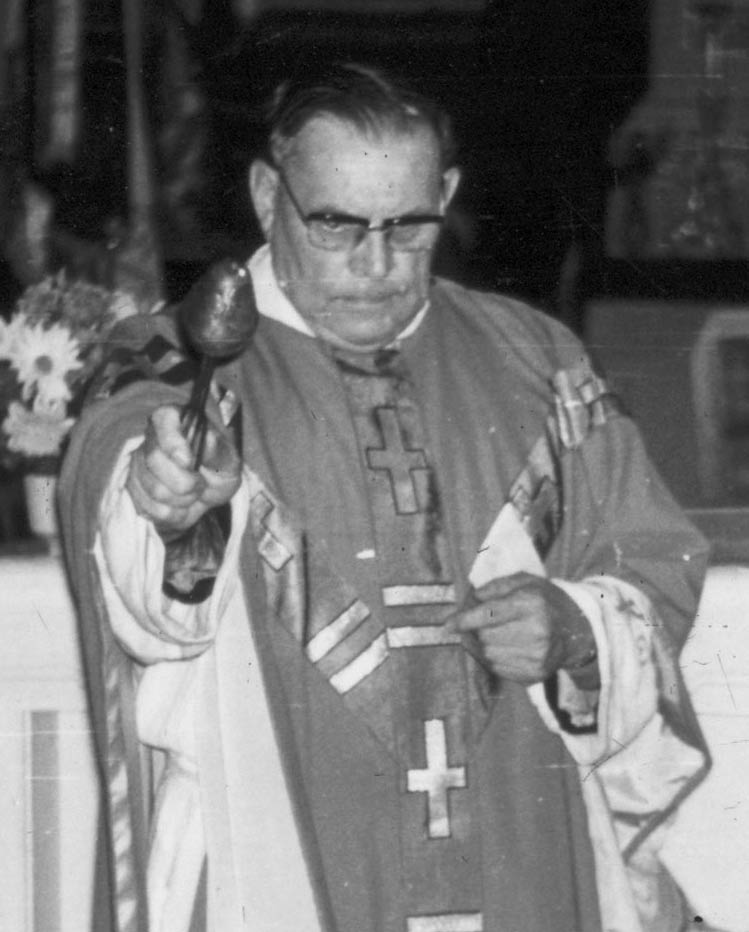
\includegraphics[width=4.835cm,height=5.992cm]{pictures/zulassungsarbeit-img051.jpg}

Abb. \stepcounter{Abb}{\theAbb}: Franz Seraph Reicheneder &

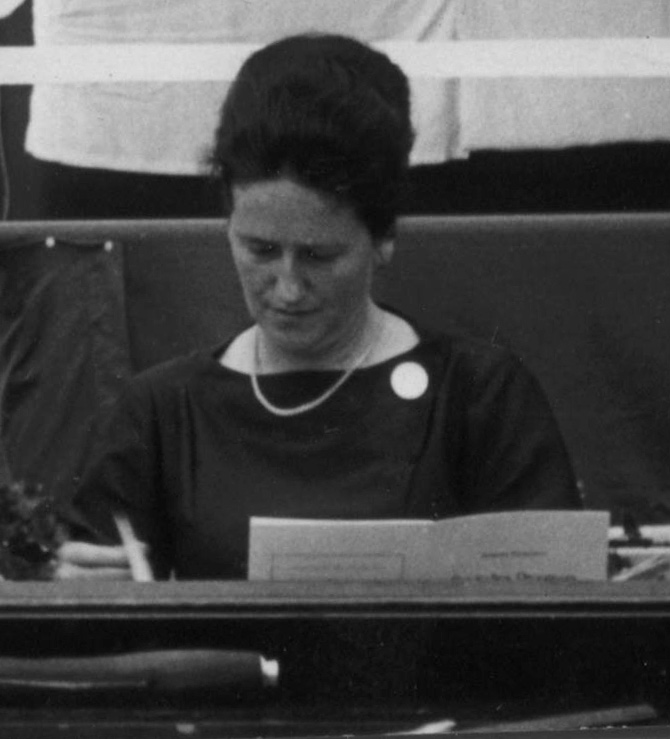
\includegraphics[width=4.484cm,height=6.003cm]{pictures/zulassungsarbeit-img052.jpg}

Abb. \stepcounter{Abb}{\theAbb}: Maria Reisinger\\
\end{supertabular}
\end{flushleft}
\end{minipage}
\end{center}
Deshalb wirkt der Brief, den Högn nach seinem Krankenhausaufenthalt am
25.1.1954 an Reicheneder schrieb, schon etwas befremdlich. Mit der
\zitat{„berechtigten Forderung auf Ruhestand auch im
Kirchenchordienst“} verkündete Högn in diesem Schreiben seinen
Rücktritt als Chorregent und Organist und bezog sich dabei nicht auf
die Folgen seines Schlaganfalls oder auf das „Kündigungsschreiben.“
 \footnote{Dokument Nr. 18, Brief von August Högn an Pfarrer
Reicheneder, 25.1.1954} In seinem Antwort-Brief vom 6.2.1954 nahm
Reicheneder zu Högns erhaltenen Brief Stellung, in dem Högn von sich
aus abdankte, und unterstrich, dass er Högns
\zitat{„Standpunkt voll und ganz verstehen“} könne, seinen
Rücktritt aber \zitat{„sehr bedauere.“ } \footnote{Dokument
Nr. 19, Brief von Pfarrer Reicheneder an August Högn, 6.2.1954}

Wären nur diese zwei Briefe und nicht zusätzlich die genauen
Erinnerungen von mehreren Zeitzeugen zur Verfügung gestanden, hätte man
eine ganz andere Schlussfolgerung daraus gezogen. Sowohl Reicheneder
als auch Högn waren daran interessiert, der Nachwelt eine andere
Version des Ausscheidens Högns als die der Kündigung durch Reicheneder
zu überlassen. Nur zwischen den Zeilen, kann man in beiden Briefen die
vorhergehenden Ereignisse erahnen, wie zum Beispiel an der Stelle, an
der Högn die \zitat{„Kündigung seitens des Hochwürdigen Herr
Pfarrers und der gleichen“} als \zitat{„blödes
Weibergeschwätz“} bewertet und darauf hinweist, dass
\zitat{„eine vertragliche Abmachung über den
Kirchenchordienst zwischen Pfarramt Ruhmannsfelden“ }und ihm niemals
bestanden hätte.“  \footnote{Dokument Nr. 18, Brief von August Högn an
Pfarrer Reicheneder, 25.1.1954}\zitat{ }Und seine angebliche
\zitat{„Stimmbandlähmung“,} \footnote{Dokument Nr. 19, Brief
von Pfarrer Reicheneder an August Högn, 6.2.1954}\zitat{ }die
Reicheneder als Entschuldigung anführte, weshalb er Högn keinen
Krankenbesuch abstattete, erscheint in diesem Zusammenhang mehr als
eine faule Ausrede.

Über den wahren Wortlaut der „Kündigungsbriefe“ ließe sich natürlich
viel spekulieren. Allein schon ihr Verschwinden ist ein Beweis für ihre
Brisanz. Reicheneder war ein passionierter Historiker und Archivar. Es
gibt wohl keinen auf die hiesige Gegend bezogenen Zeitungsartikel aus
Reicheneders Ruhmannsfeldener Zeit, der nicht in seine über 30 prall
gefüllte Ordner umfassende „Chronik Ruhmannsfelden“ angefügt wurde.
Auch seine Korrespondenz dokumentierte Reicheneder sehr genau. Viele
von ihm verfasste Briefe lassen sich im Pfarrarchiv im
Kohlepapierabdruck nachlesen, wie etwa das Schreiben an Högn vom
6.2.1954. Die „Kündigungsschreiben“ hat Reicheneder ganz bewusst nicht
archiviert, damit kein schlechtes Licht auf ihn fällt. Einen kaum
unwürdigeren Abschied hätte Reicheneder Högn nach 43 Jahren Dienstzeit
an der Kirchenmusik in Ruhmannsfelden nicht bieten können.

Diese ungerechte Vorgehensweise von Reicheneder gegenüber Högn ist kein
Einzelfall. Ein Ereignis wenige Jahre später ist bezeichnend für
Reicheneders Problemlösungsstrategie mit der „Brechstange“: Nachdem
Pfarrer Reicheneder bei einer Sonntags-Predigt von der Kanzel aus unter
anderem über die \zitat{„Leistungsabzeichen für nächtliche
Liebesfahrten“} \footnote{
http://home.vrweb.de/pfarrei.ruhmannsfelden/reichene.htm} wetterte, die
am Fußballer Ball 1957 verliehen wurden, ließen sich die Beschuldigten
nicht zurechtweisen und veranstalten, nach Angaben des Geistlichen
selbst, aus einer Trotzreaktion heraus ein Faschingsbegräbnis am
Aschermittwoch mit Musik und Saufgelage. \zitat{„Bis die
Haupträdelsführer beim Pfarramt vorstellig geworden sind“;}\footnote{
http://home.vrweb.de/pfarrei.ruhmannsfelden/reichene.htm} wie es in
einer Pressemitteilung des Pfarramts hieß, sollten nun die Glocken in
Ruhmannsfelden schweigen. Diese Aktion machte natürlich nicht nur in
der regionalen Presse ihre Runde. Die Glocken läuteten erst wieder, als
sich der Bürgermeister von Ruhmannsfelden in den Fall einbezog und für
eine Lösung des Problemfalls sorgte, die schriftlich festgehalten
wurde.\footnote{
http://home.vrweb.de/pfarrei.ruhmannsfelden/reichene.htm}

In der Kirchenverwaltungssitzung vom 21.2.1954 wurde Högns Nachfolge
endgültig geregelt. Maria Reisinger erhielt die Organistenstelle und
Franz Danziger übernahm die Chorleitung. \footnote{Dokument Nr. 124,
Protokoll der Kirchenverwaltungssitzung, 21.2.1954}

\subsection{Die letzten Lebensjahre}

\hypertarget{RefHeadingToc100333738}{}  [Warning: Image ignored]
% Unhandled or unsupported graphics:
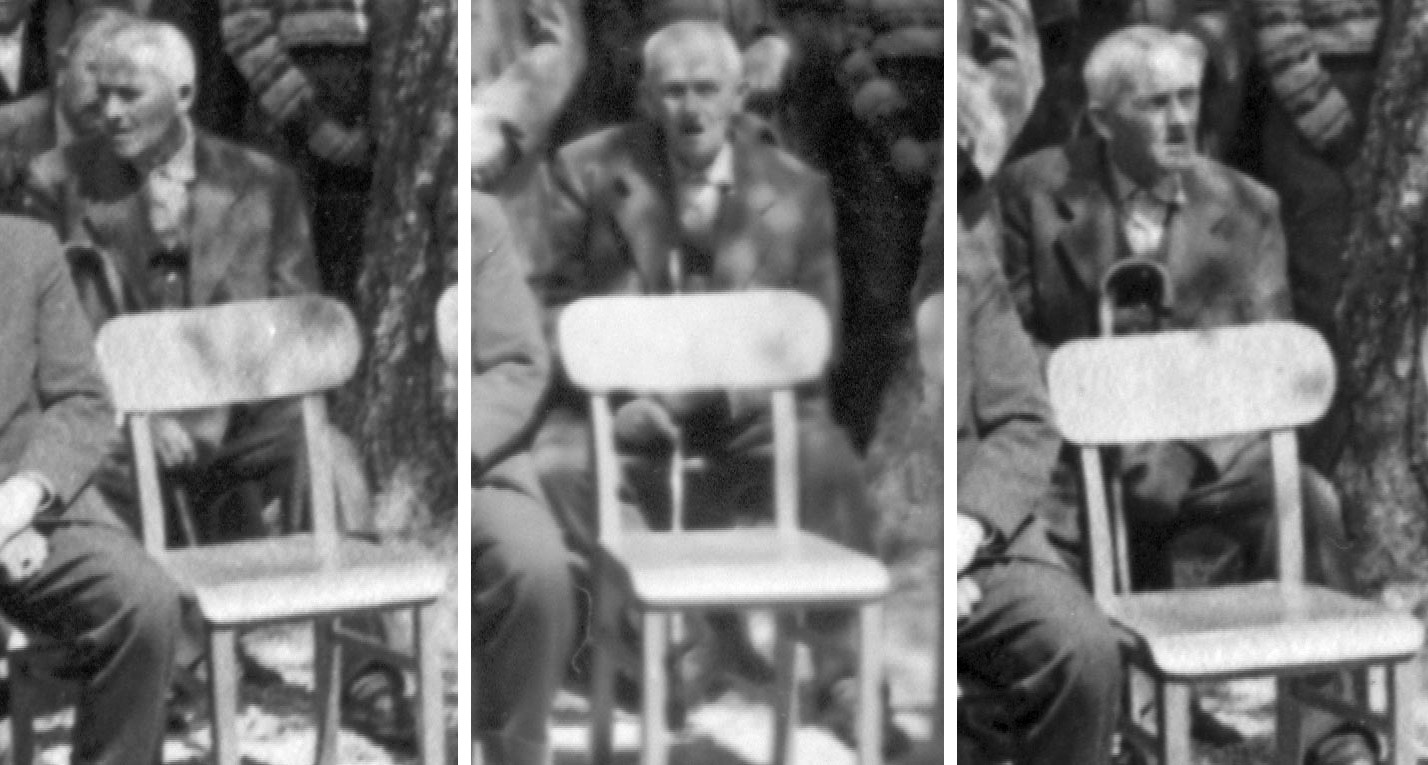
\includegraphics[width=15.981cm,height=8.56cm]{pictures/zulassungsarbeit-img053.jpg}


Abb. \stepcounter{Abb}{\theAbb}: August Högn auf Bildern, die zur
Einweihung des Schulanbaus an Christihimmelfahrt 1959 aufgenommen
wurden.

Einen tiefen Einschnitt in Högns unruhiges Rentnerleben stellte sein
Schlaganfall Ende 1953 dar. Sein Ruhestand, der eigentlich schon 1945
mit der Suspendierung vom Schuldienst infolge der Entnazifizierung
begann und nur durch einen kurzen Schuleinsatz 1947 \footnote{Dokument
Nr. 48, Zeitungsartikel aus Viechtacher Bayerwald-Bote, 2.8.1958}
unterbrochen wurde, konnte vor 1953 wohl kaum als solcher bezeichnet
werden, wenn man seine Aktivitäten für die Kirche und Heimatkunde
betrachtet.

Vieles spricht dafür, dass Högn trotz seiner körperlichen
Beeinträchtigungen ab 1954 ein aktives Leben führte. Er war sogar noch
schöpferisch tätig, wie sein Marienlied „Ruf an die Christenheit“
beweist, das zur 300. Jahrfeier des Osterbrünnls 1960 entstanden ist.
Einige weltliche Kompositionen, die nicht erhalten sind, hat Högn nach
seinem 80. Geburtstag für den Ruhmannsfeldener Männerchor
geschrieben. \footnote{Dokument Nr. 49, Zeitungsartikel aus Viechtacher
Bayerwald-Bote, 5.8.1958; Interview Nr. 24, Johann Glasschröder,
28.12.2004, Absatz 32} Auf eine rege Korrespondenz lassen die vier
langen Briefe schließen, die Högn einem ehemaligen Schüler bis nach
Australien schickte. Sein großes Interesse am öffentlichen Leben in
Ruhmannsfelden belegen die vielen Details aus dem Ortsgeschehen, die
Högn in die Briefe mit einfließen ließ. Kurz vor seinem Tod kaufte er
sich einen Fernsehapparat und konnte sich so über die Außenwelt
informieren. \footnote{Dokument Nr. 73, Brief von August Högn an
Stephan Leitner, 10.3.1961}

In seinen letzten Briefen kommt ein gewisser Schwermut deutlich zum
Ausdruck. Selbst Feste wie Weihnachten findet er
\zitat{„langweilig und ohne Abwechslung“ } \footnote{Dokument
Nr. 70, Brief von August Högn an Stephan Leitner, 9.1.1960} und beklagt
sich, dass der Fasching in Ruhmannsfelden \zitat{„ziemlich
mau“} \footnote{Dokument Nr. 71, Brief von
August Högn an Stephan Leitner, 15.3.1960}\zitat{ }war.
Sehnsucht nach seiner an der Donau gelegenen Heimatstadt Deggendorf
macht sich breit, wenn er schreibt: \zitat{„An den Bergen des
bayerischen Waldes habe ich schon genug. Möchte lieber hinaus in die
Ebene, an die Donau, zum Wasser.“}\footnote{
Dokument Nr. 72, Brief von August Högn an Stephan Leitner, Dez. 1960}
Seine Gedanken scheinen oft um den Tod zu kreisen, wenn er als
Neuigkeit schon zu Beginn eines Briefes mehre Todesfälle aufzählt und
resümiert: \zitat{„Bei uns hier ist die Sterblichkeit
ziemlich groß.“ } \footnote{Dokument Nr. 72, Brief von August Högn an
Stephan Leitner, Dez. 1960}

\begin{center}
\begin{minipage}{9.146cm}
\begin{center}
\tablefirsthead{}
\tablehead{}
\tabletail{}
\tablelasttail{}
\begin{supertabular}{m{4.309cm}m{4.4370003cm}}

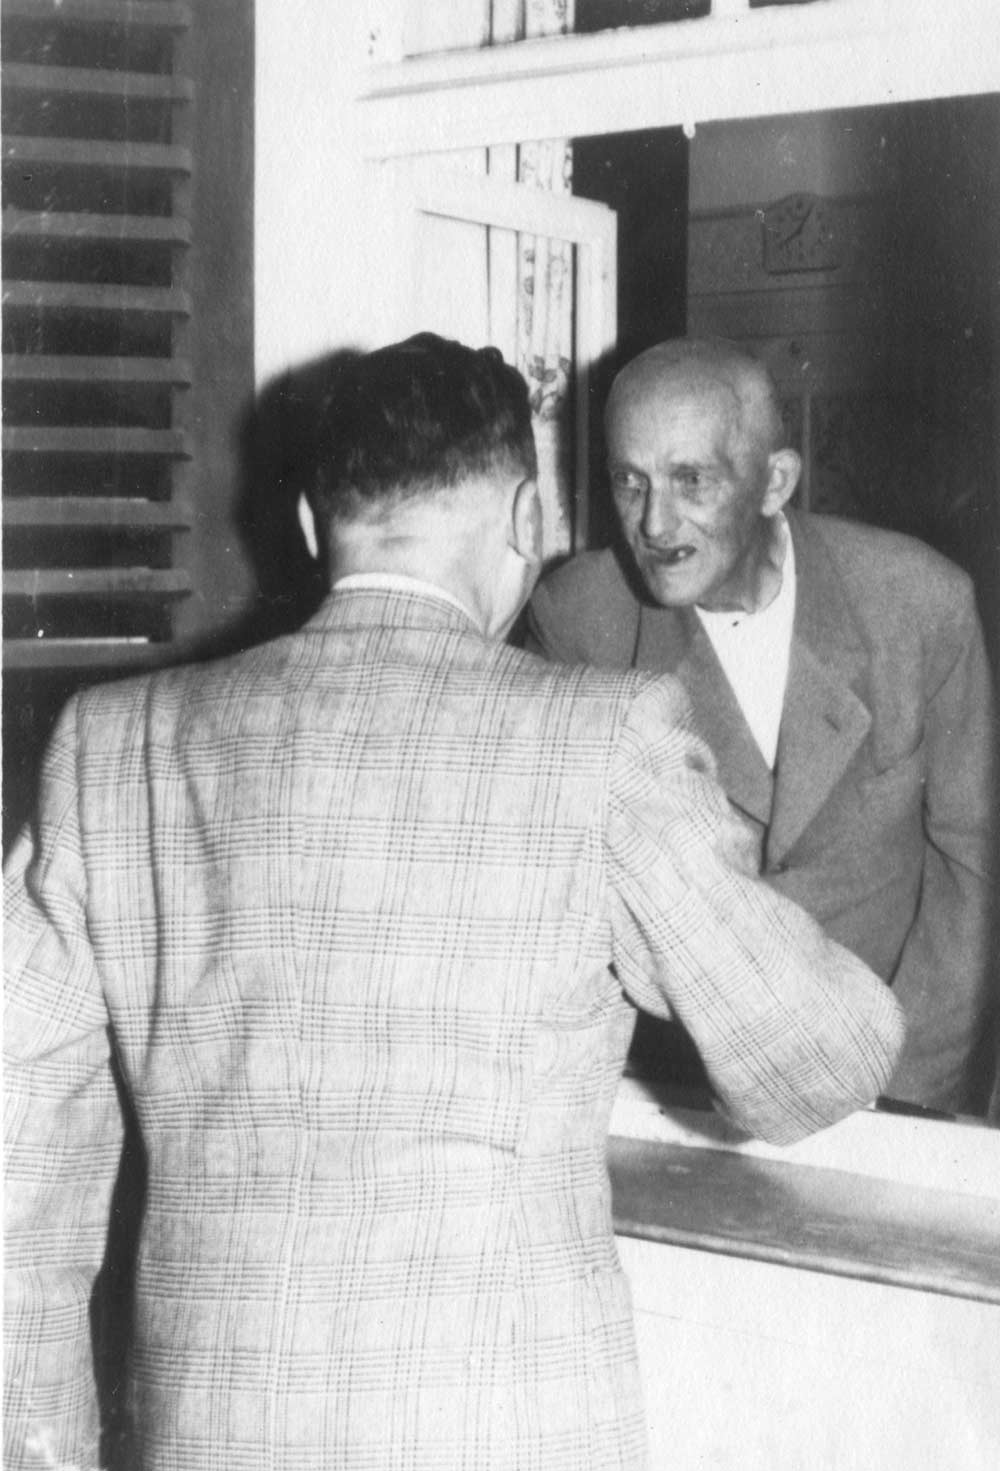
\includegraphics[width=4.128cm,height=6.071cm]{pictures/zulassungsarbeit-img054.jpg}

Abb. \stepcounter{Abb}{\theAbb}: Franz Danziger gratuliert August Högn
am Vorabend zu seinem 80. Geburtstag &

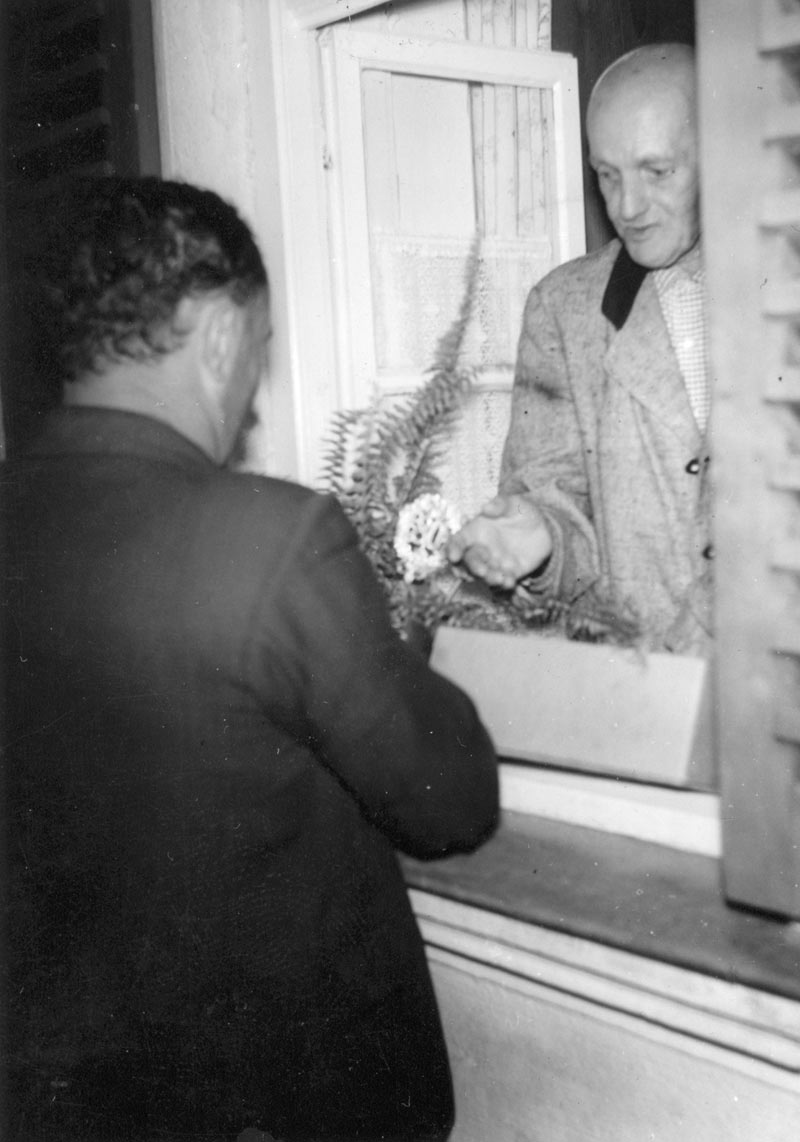
\includegraphics[width=4.255cm,height=6.073cm]{pictures/zulassungsarbeit-img055.jpg}

Abb. \stepcounter{Abb}{\theAbb}: Der Zachenberger Bürgermeister
Bielmeier überreicht August Högn einen Geschenkkorb zum 80.
Geburtstag\\
\end{supertabular}
\end{center}
\end{minipage}
\end{center}
Ende 1960 scheint sich Högns Gesundheitszustand zu verschlechtern. Er
beklagt sich, dass das sein \zitat{„gesundheitliches Befinden
nicht das beste“} ist und das \zitat{„Marschieren sehr
schlecht geht.“ }Um Besserung zu erfahren, sucht er sogar einen Arzt im
mehr als 50 km entfernten Straubing auf. \footnote{Dokument Nr. 72,
Brief von August Högn an Stephan Leitner, Dez. 1960} Er ist immer mehr
auf Hilfe anderer angewiesen und seine Haushälterin Rosa Beischmied
wird zur \zitat{„Krankenfürsorgerin.“ } \footnote{Dokument
Nr. 73, Brief von August Högn an Stephan Leitner,
10.3.1961}Ein letztes Foto von Högn vom Juli
1961 zeigt zwar einen hageren, alten Mann, der an den Folgen seines
Schlaganfalles sichtbar leidet, doch es zeigt keinen vom Tode
gekennzeichneten Mann, der wenige Monate später sterben wird.

August Högn starb am 13. Dezember 1961 um 5 Uhr morgens.\footnote{
Dokument Nr. 50, Zeitungsartikel aus dem Viechtacher Bayerwald-Bote,
14.12.1961} Sein Tod kam nicht plötzlich, da er rechtzeitig mit den
Sterbesakramenten versehen worden war. \footnote{Dokument Nr. 50,
Zeitungsartikel aus dem Viechtacher Bayerwald-Bote, 14.12.1961} Nach
Aussagen von Högns Enkelin Gertraud von Molo war er bis kurz vor seinem
Tod rüstig \footnote{Interview Nr. 20, Gertraud von Molo, 23.11.2004,
Absatz 14} und sein Tod dürfte auf eine eher \zitat{„kürzere
Krankheit“ } \footnote{Interview Nr. 2, Barbara Essigmann, 27.12.2002,
Absatz 62} zurückzuführen sein, als auf eine \zitat{„lange
schwere“}  \footnote{Dokument Nr. 51, Zeitungsartikel aus Viechtacher
Bayerwald-Bote, 15.12.1961} Krankheit, wie es im seinem Nachruf im
Viechtacher Bayerwald-Boten steht. Im Sterberegister der Pfarrei
Ruhmannsfelden steht als Todesursache „Herzinsuffizienz“, was eher auf
einen plötzlichen Tod schließen lässt. \footnote{Dokument Nr. 112,
Eintrag im Sterberegister des Pfarramts Ruhmannsfelden, 13.12.1961}
Waren bei der Überführung des Leichnams am Todestag anwesend\footnote{
Dokument Nr. 51, Zeitungsartikel aus Viechtacher Bayerwald-Bote,
15.12.1961} nur wenige enge Freunde, die dem Leichenauto Richtung
Deggendorf einige hundert Meter folgten, \footnote{Interview Nr. 2,
Barbara Essigmann, 27.12.2002, Absatz 64} so dürfte es beim im
Ruhmannsfelden abgehaltenen Requiem am darauffolgenden Tag in
Ruhmannsfelden ein Großteil der Ruhmannsfeldener Bevölkerung gewesen
sein, der von Högn Abschied nahm. Die Ruhmannsfeldener Volksschule nahm
an der Trauerfeier teil und jeder ehemalige Schüler erhielt eine
Einladung zum Besuch des Trauergottesdienstes. \footnote{Dokument Nr.
50, Zeitungsartikel aus dem Viechtacher Bayerwald-Bote, 14.12.1961} Die
offizielle Beerdigung fand am 15. Dezember in der Deggendorfer
Pfarrkirche Mariä Himmelfahrt statt. \footnote{Dokument Nr. 66,
Todesbenachrichtigung, 13.12.1961} Bei eisiger Kälte\footnote{
Interview Nr. 3, Ida Högn, 29.12.2002, Absatz 20} hielten die Lehrer
Karl Schambeck, \footnote{Dokument Nr. 52, Brief von Elfriede
Schlumprecht an Lehrer Schambeck, 3.1.1962} Franz Nemetz\footnote{
Interview Nr. 3, Ida Högn, 29.12.2002, Absatz 20; Dokument Nr. 53,
Brief von Elfriede Schlumprecht an Rektor Langesee, 3.1.1962} und der
Kreisschulrat Botschafter \footnote{Dokument Nr. 53, Brief von Elfriede
Schlumprecht an Rektor Langesee, 3.1.1962} am Grab Trauerreden auf
August Högn. Besonders die Ansprache von Lehrer Nemetz blieb als eine
sehr lange Rede bei vielen Anwesenden in Erinnerung.\footnote{
Interview Nr. 3, Ida Högn, 29.12.2002, Absatz 20} Abordnungen der
Vereine aus Ruhmannsfelden waren mit Fahnen anwesend und eine
Bläsergruppe der freiwilligen Feuerwehr von Ruhmannsfelden spielte für
ihr Ehrenmitglied zum Abschied das Lied „Wir hatten einen Kameraden.“
 \footnote{Interview Nr. 20, Gertraud von Molo, 23.11.2004, Absatz 42}
August Högn fand seine letzte Ruhestätte auf dem Deggendorf Friedhof,
im schönen Grabmal \footnote{Interview Nr. 20, Gertraud von Molo,
23.11.2004, Absatz 10} neben seiner 1926 verstorbenen Ehefrau Emma.

\begin{center}
\begin{minipage}{5.542cm}
\begin{flushleft}
\tablefirsthead{}
\tablehead{}
\tabletail{}
\tablelasttail{}
\begin{supertabular}{m{5.342cm}}

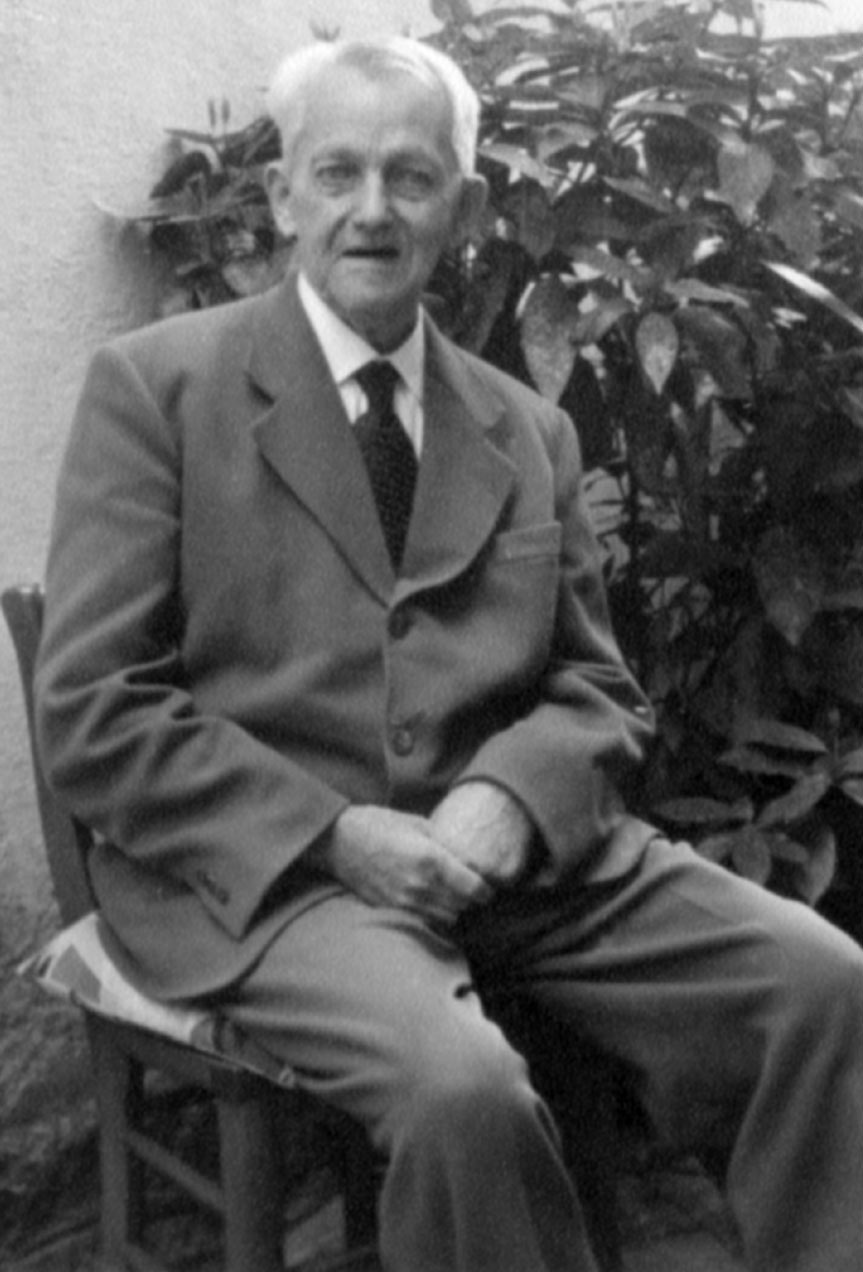
\includegraphics[width=5.159cm,height=7.606cm]{pictures/zulassungsarbeit-img056.jpg}

Abb. \stepcounter{Abb}{\theAbb}: letztes Foto von August Högn, Juli
1961\\
\end{supertabular}
\end{flushleft}
\end{minipage}
\end{center}
\begin{flushleft}
\tablefirsthead{}
\tablehead{}
\tabletail{}
\tablelasttail{}
\begin{supertabular}{m{12.311cm}m{3.6929998cm}}

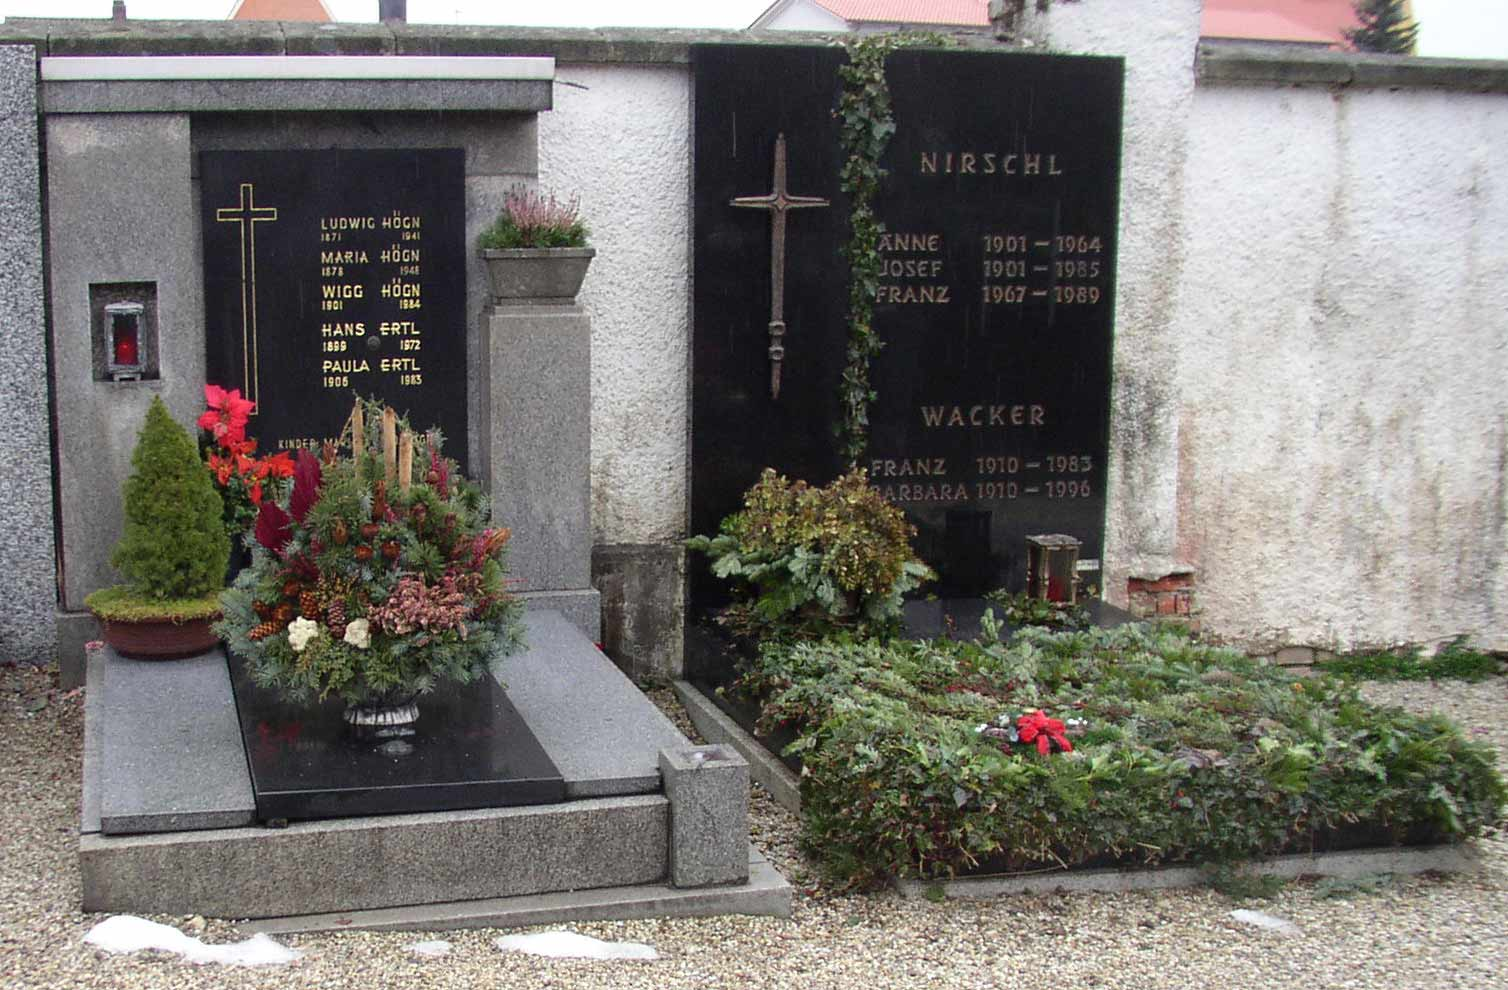
\includegraphics[width=12.129cm,height=8.015cm]{pictures/zulassungsarbeit-img057.jpg}

Abb. \stepcounter{Abb}{\theAbb}: Familiengrab von Ludwig Högn (links)
und ehemalige Grabstätte von August Högn und seiner Ehefrau (rechts),
heute im Besitz der Familie Nirschl &

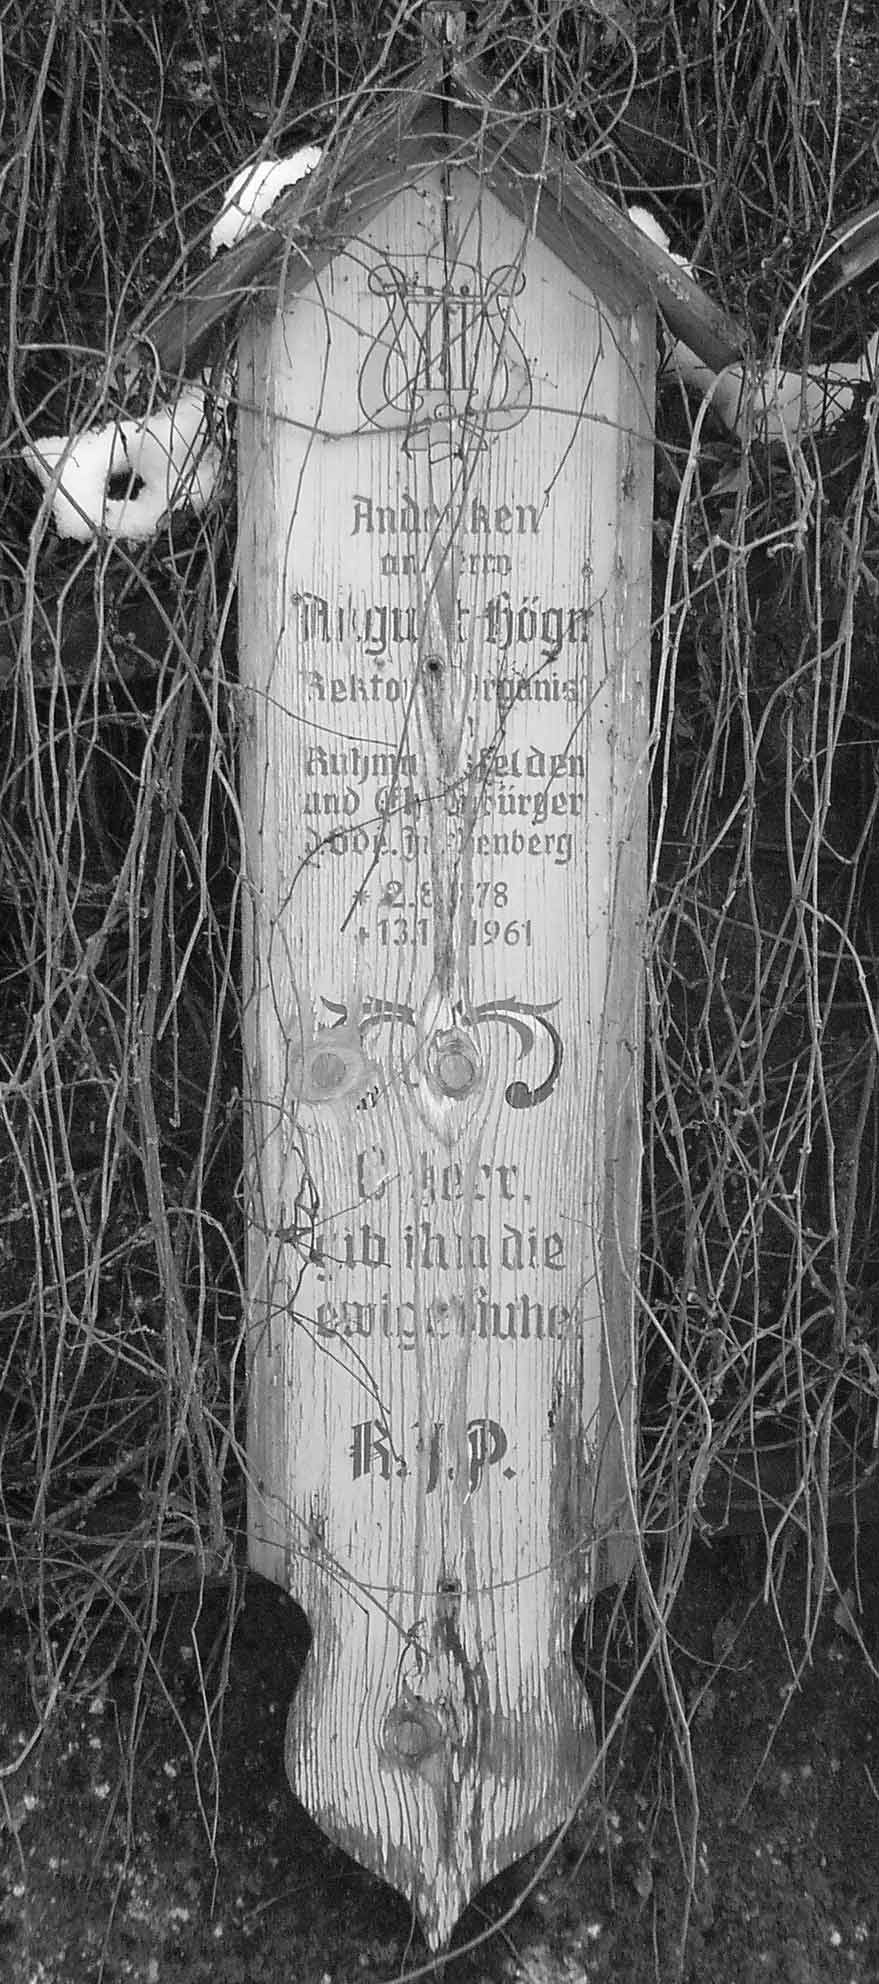
\includegraphics[width=3.51cm,height=7.978cm]{pictures/zulassungsarbeit-img058.jpg}

Abb. \stepcounter{Abb}{\theAbb}: Totenbrett zum Andenken von August Högn
an der Wallfahrtskirche Osterbrünnl in Ruhmannsfelden\\
\end{supertabular}
\end{flushleft}





\end{document}
